
\documentclass[12pt]{article}


\usepackage{fancyhdr}

\usepackage{enumitem}

\usepackage{longtable}
\usepackage{lmodern}

\usepackage{placeins}


\usepackage{algorithm}
\usepackage{algpseudocode}

\usepackage{float}
\floatstyle{plain}
\restylefloat{figure}

\usepackage[a4paper,top=3cm,bottom=3cm,left=3cm,right=3cm]{geometry}

\usepackage{ccfonts} 

\usepackage[english]{babel}

\usepackage{ucs}

\usepackage{listings}

\usepackage[T1]{fontenc}

\usepackage{amsmath,amssymb}
\usepackage{xspace,hyphenat}
\usepackage{calc}

\usepackage{textcomp}
\usepackage{eurosym}

\usepackage{url}
\usepackage{amssymb}
\usepackage{caption}
\captionsetup{format=plain, labelfont=bf, justification=centering, singlelinecheck=false} 
\usepackage{subcaption}
\usepackage{natbib}


\newcommand{\inputfigure}[2]{\resizebox{#1}{!}{\input{pics/#2.pdftex_t}}}




\pdfoutput=1
\usepackage[pdftex]{graphicx, color, rotating}


\usepackage[pdftex=true, bookmarks=true, colorlinks=true, bookmarksnumbered=true,
plainpages=false]{hyperref}
\usepackage[acronym, nonumberlist, nogroupskip, nopostdot]{glossaries}

\hypersetup{
    colorlinks=true,
    linkcolor=blue,       % color of internal links
    citecolor=red,        % color of links to bibliography
    filecolor=magenta,    % color of file links
    urlcolor=cyan         % color of external links
}


\graphicspath{{./bilder/}}
\DeclareGraphicsExtensions{.jpg,.png,.pdf}
\pdfcompresslevel=9
\pdfinfo{
  /Title (Bachelor Thesis)
  /Author (Joaquin Arias)
  /Subject (Bachelor Thesis)
}

\makeglossaries
\newacronym{ea}{EA}{Evolutionary Algorithms}
\newacronym{qd}{QD}{Quality-Diversity}
\newacronym{mo}{MO}{Multi Objective}
\newacronym{mome}{MOME}{Multi Objective MAP-Elites}
\newacronym{mome-pgx}{MOME-PGX}{Multi-Objective MAP-Elites with Policy-Gradient Assis- tance and Crowding-based Exploration}
\newacronym{drl}{DRL}{Deep Reinforcement Learning}
\newacronym{mdp}{MDP}{Markov Decision Process}
\newacronym{td3}{TD3}{Twin Delayed Deep Deterministic}
\newacronym{ga}{GA}{Genetic Algorithm}
\newacronym{pg}{PG}{Policy Gradient}

\begin{document}

%%%%%%%%%%%%%%%%%%COVER PAGE%%%%%%%%%%%%%%%%%%%%%%%%%%%%%%%%%%
\pagenumbering{roman}
\textheight600pt
\topmargin0pt
\voffset0pt
\selectlanguage{english}
\headheight100pt
\headsep=100pt
\footskip=50pt
\sloppy

\title{
\vspace{4cm}
\LARGE{\textbf{Enhancing Robustness and Adaptability in Robotic Systems: A Quality-Diversity Approach to Addressing Wrong Initial Simulation Parameters and Optimizing Model Parameters}}\\ 
\vspace{0.5cm}
\large{by}

}
\author{
\vspace{0.5cm}
\textbf{Joaquin Arias}\\
\\
\normalsize{Bachelor Thesis in Robotics and Intelligent Systems}\\
}


\lhead{ 

\includegraphics[width=0.5\textwidth]{Bilder/dfki}%
\includegraphics[width=0.5\textwidth]{Bilder/Constructor}
}
\date{}

\maketitle

\vspace{4.5cm}
\begin{center}
\normalsize{\textbf{Submission Date:} \today}
\end{center}

\noindent\begin{minipage}[b]{0.5\textwidth}
    \flushleft
    \textbf{1st Examiner:} \\
    Prof. Dr. Dr. h.c. Frank Kirchner \\
    \vspace{0.3cm}
    \textbf{2nd Examiner:} \\
    Prof. Dmitry Kropotov
\end{minipage}%
\begin{minipage}[b]{0.5\textwidth}
    \flushright
    \textbf{Supervisors:} \\
    M.Sc. Marc Otto \\
    Prof. Dr. Dr. h.c. Frank Kirchner
\end{minipage}
\:
\hrule
  \begin{center}
    Constructor University $|$ School of Computer Science and Engineering
  \end{center}



\thispagestyle{fancy}

\headheight0pt
\headsep20pt
\footskip36pt
\newpage
%%%%%%%%%%%%%%%%%%STATUTORY DECLARATION%%%%%%%%%%%%%%%%%%%%%%%%%%%%%%%%%%
\vspace{1cm}

\begin{center}
    \textbf{STATUTORY DECLARATION}
\end{center}
\noindent
\begin{tabular}{|p{0.45\textwidth}|p{0.5\textwidth}|}
    \hline
    \textbf{Family Name, Given/First Name} & Arias, Joaquin \\
    \hline
    \textbf{Matriculation number} & 30005300 \\
    \hline
    \textbf{Kind of thesis submitted} & Bachelor Thesis \\
    \hline
\end{tabular}


\vspace{1cm}

\noindent\textbf{English: Declaration of Authorship}

\vspace{0.5cm}

\noindent I hereby declare that the thesis submitted was created and written solely by myself without any external support. Any sources, direct or indirect, are marked as such. I am aware of the fact that the contents of the thesis in digital form may be revised with regard to usage of unauthorized aid as well as whether the whole or parts of it may be identified as plagiarism. I do agree my work to be entered into a database for it to be compared with existing sources, where it will remain in order to enable further comparisons with future theses. This does not grant any rights of reproduction and usage, however.

\noindent This document was neither presented to any other examination board nor has it been published.
\\

\noindent\textbf{German: Erklärung der Autorenschaft (Urheberschaft)}

\vspace{0.5cm}

\noindent Ich erkläre hiermit, dass die vorliegende Arbeit ohne fremde Hilfe ausschließlich von mir erstellt und geschrieben worden ist. Jedwede verwendeten Quellen, direkter oder indirekter Art, sind als solche kenntlich gemacht worden. Mir ist die Tatsache bewusst, dass der Inhalt der Thesis in digitaler Form geprüft werden kann im Hinblick darauf, ob es sich ganz oder in Teilen um ein Plagiat handelt. Ich bin damit einverstanden, dass meine Arbeit in einer Datenbank eingegeben werden kann, um mit bereits bestehenden Quellen verglichen zu werden und dort auch verbleibt, um mit zukünftigen Arbeiten verglichen werden zu können. Dies berechtigt jedoch nicht zur Verwendung oder Vervielfältigung.

\noindent Diese Arbeit wurde noch keiner anderen Prüfungsbehörde vorgelegt noch wurde sie bisher veröffentlicht.

\vfill

\noindent\makebox[\textwidth]{\dotfill}\\
Date, Signature

\newpage
%%%%%%%%%%%%%%%%%%ABSTRACT%%%%%%%%%%%%%%%%%%%%%%%%%%%%%%%%%%%%%%%%%%%
\begin{abstract}
Robots must quickly adapt to new and unexpected situations when they are placed in unfamiliar environments. In critical scenarios where human expertise cannot always be leveraged due to model inaccuracies or time constraints, it is essential for the robot to quickly adapt to ensure mission success. This research focuses on enhancing robotic adaptability by using the state-of-the-art algorithm MOME-PGX, which equips robots with a wide range of behaviors. When faced with unknown challenges, a separate adaptation method is employed to select the best actions from the pre-learned behaviors.

In this study, a robotic scenario was simulated, in which the kick of a ball to a target was tested. When encountering moderate changes in surface friction or physical obstacles, these adaptation techniques allowed the robot to adapt and find suitable alternative behaviors within just a few trials. Additionally, encouraging the robot to explore its surroundings by interacting with the ball for different durations accelerated the learning of diverse behaviors that can be useful for tasks like keeping the ball stable or providing the robot with a better understanding of the environment.

This work demonstrates the potential of these algorithms to make robots more autonomous in dynamic and unpredictable environments, especially on situations where the speed of adaptation is essential.

\end{abstract}

\newpage

%%%%%%%%%%%%%%%%%%CONTENTS%%%%%%%%%%%%%%%%%%%%%%%%%%%%%%%%%%%%%%%%%%%


 \tableofcontents

 \clearpage
\pagenumbering{arabic}

%%%%%%%%%%%%%%%%%%INTRODUCTION%%%%%%%%%%%%%%%%%%%%%%%%%%%%%%%%%%%%%%%%%%%

\section{Introduction}

Natural selection and evolution are Darwinian concepts that refer to the process by which an organism that is better adapted to its environment is more likely to survive and produce offspring, causing evolution of the species over time. This same concept has been applied to Artificial Intelligence through Evolutionary Algorithms (EAs). By exploring solutions through genetic operators, EAs are able to run a "natural selection" process where the less fit solutions die off, and the most fit ones are used for genetic expansion \citep{Soni_2021}. EAs and other search algorithms traditionally focus on pure optimization \citep{Cully_Mouret_Doncieux_2019}: they aim to find the \textit{single} fittest solution for a given objective \citep{qian2024quality}.

In real life environments, robots face challenges, such as damage or obstacles, that require them to quickly adapt to be able to carry out their task effectively. In these cases, the traditional optimization methods are not practical since they often require human supervision in case of failure, making them inefficient in terms of time and labor \citep{kober2013reinforcement}. An approach that has shown to be useful for improving robots adaptation is the use of Quality Diversity (QD) algorithms. They are a type of EA, but instead of finding a single solution like EAs traditionally do, they generate a large set of diverse and high quality solutions \citep{Cully_Mouret_Doncieux_2019}. In the previous study \textit{Robots that can adapt like animals}, it was demonstrated that learning a repertoire of solutions, helped robots to adapt in under two minutes in case of damage \citep{cully2015robots}.

Having a repertoire of solutions generated by QD algorithms is useful because if one solution fails, another is immediately available without needing to be learned first. In more complex scenarios, it may be desired to take into account more than one objective. For such cases, multi-objective optimization can be implemented within MAP-Elites, which constitute a part of QD algorithms that stores solutions in a multi-dimensional grid. In multi-objective optimization, there is no single solution that works equally well for all the objectives, so a trade-off of objectives is considered. This is known as Pareto front. The algorithm that integrates multi-objective optimization into MAP-Elites is known as MOME and it stores Pareto fronts of solutions in each cell \citep{mouret2015illuminating}. 

A new algorithm, MOME-PGX, has been introduced, which is between 4.2 and 43 times more data efficient than MOME by incorporating policy-gradient assistance and crowding-based exploration within MOME \citep{janmohamed2023improving}. This algorithm is used in this research to explore the adaptability of robotic systems, which is increasingly important for robots to autonomously interact with the environment, improve existing skills, or gain new ones \citep{nolfi2022progress}. 

The first aspect that this project aims at researching is the sensibility of QD algorithms to inaccuracies in the simulation model that the robot is trained on. This  addresses the research question: \textit{To what extent do inaccuracies in the simulation model impact the performance of QD algorithms?} Furthermore, the project also evaluates a way to improve the model more efficiently by answering the second research question: \textit{Can the model be improved faster and more efficiently by leveraging the exploration behaviors learned during the process?}
 

\section{Background}
\subsection{Quality Diversity Algorithms}
Evolutionary Algorithms and other search algorithms are traditional optimization methods that aim to look in a search space $\mathcal{X}$ for a single, high-performing solution $x$ to the given problem by maximizing an objective function $f:\mathcal{X} \rightarrow \mathbb{R}$ \citep{qian2024quality}. On the other hand, QD algorithms use a descriptor function $\mathbf{b}:\mathcal{X} \rightarrow \mathbb{R}^{d}$ which maps the solutions to $d$-dimensional descriptor vectors that describe the behavior of the respective solution. QD algorithms generate a large set of diverse and high-performing solutions $x_{i} \in \mathcal{X}$ by finding solutions that maximize $f$ and have diverse descriptor vectors \citep{janmohamed2023improving}. 

MAP-Elites is the most popular QD algorithm \citep{qian2024quality}, where all the possible behavior descriptors $S=\mathbf{b}(\mathcal{X})$, also known as the feature space or descriptor space, is discretized into a grid with $m$ cells, and in each cell $S_i$ corresponding to the descriptor $\mathbf{b}(x_{i})$, a solution $x_i$ is stored \citep{janmohamed2023improving}. The performance is measured with the QD score (Equation \ref{eq:qd_score}), which corresponds to the total fitness across all the occupied cells; the higher the score, the closer the robot is to successfully completing the given task \citep{pugh2015confronting}. 
\begin{equation}
\label{eq:qd_score}
\sum\limits_{i=1}^m f(x_i), \ \text{where} \ \forall i, \ \mathbf{b}(x_i) \in S_i. 
\end{equation}
The goal of QD algorithms is to maximize the QD score, which implies finding solutions $x_{i} \in \mathcal{X}$ where each $x_{i}$ is in a different cell $S_i$ and optimizes the objective function within that cell \citep{pierrot2022multi}:
\begin{equation}
\label{eq:qd_problem}
\max\limits_{x \in \mathcal{X}} \sum\limits_{i=1}^m f(x_i), \ \text{where} \ \forall i, \ \mathbf{b}(x_i) \in S_i. 
\end{equation}

To better understand the discretization of the descriptor space an example from the study \textit{Robots that can adapt like animals} by \citet{cully2015robots} is presented. In this study, the researchers investigated how a hexapod robot could adapt in the case of damage. One of the behavior descriptors chosen by the researchers was the proportion of time each leg is in contact with the ground. Therefore, the descriptor vectors are six dimensional vectors, where each dimension corresponds to each leg and it was discretized as in Figure \ref{fig:6dgrid}.

\begin{figure}[H]
    \centering
    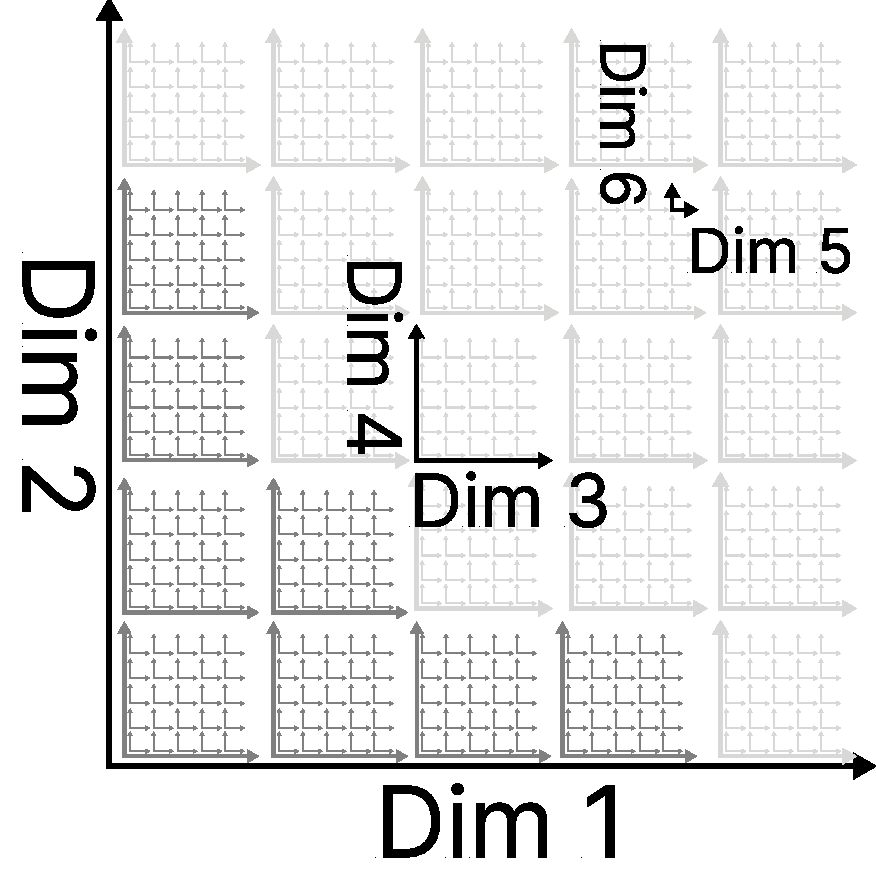
\includegraphics[width=0.3\textwidth]{Bilder/hexa_grid}
    \caption{Discretization of the behavior descriptors into a 6 dimensional grid, with one behavior descriptor per robot leg \citep{cully2015robots}.}
    \label{fig:6dgrid}
\end{figure}

The MAP-Elites algorithm (Figure \ref{fig:map-elites}) starts by selecting a set of random solutions. Then they are mutated and the performance of each new solution is recorded. The mutated solutions are added back to the grid if the respective cell is empty or if the performance of the new solution is higher than the solution occupying the cell \citep{mouret2015illuminating}. 
\begin{figure}[H]
    \centering
    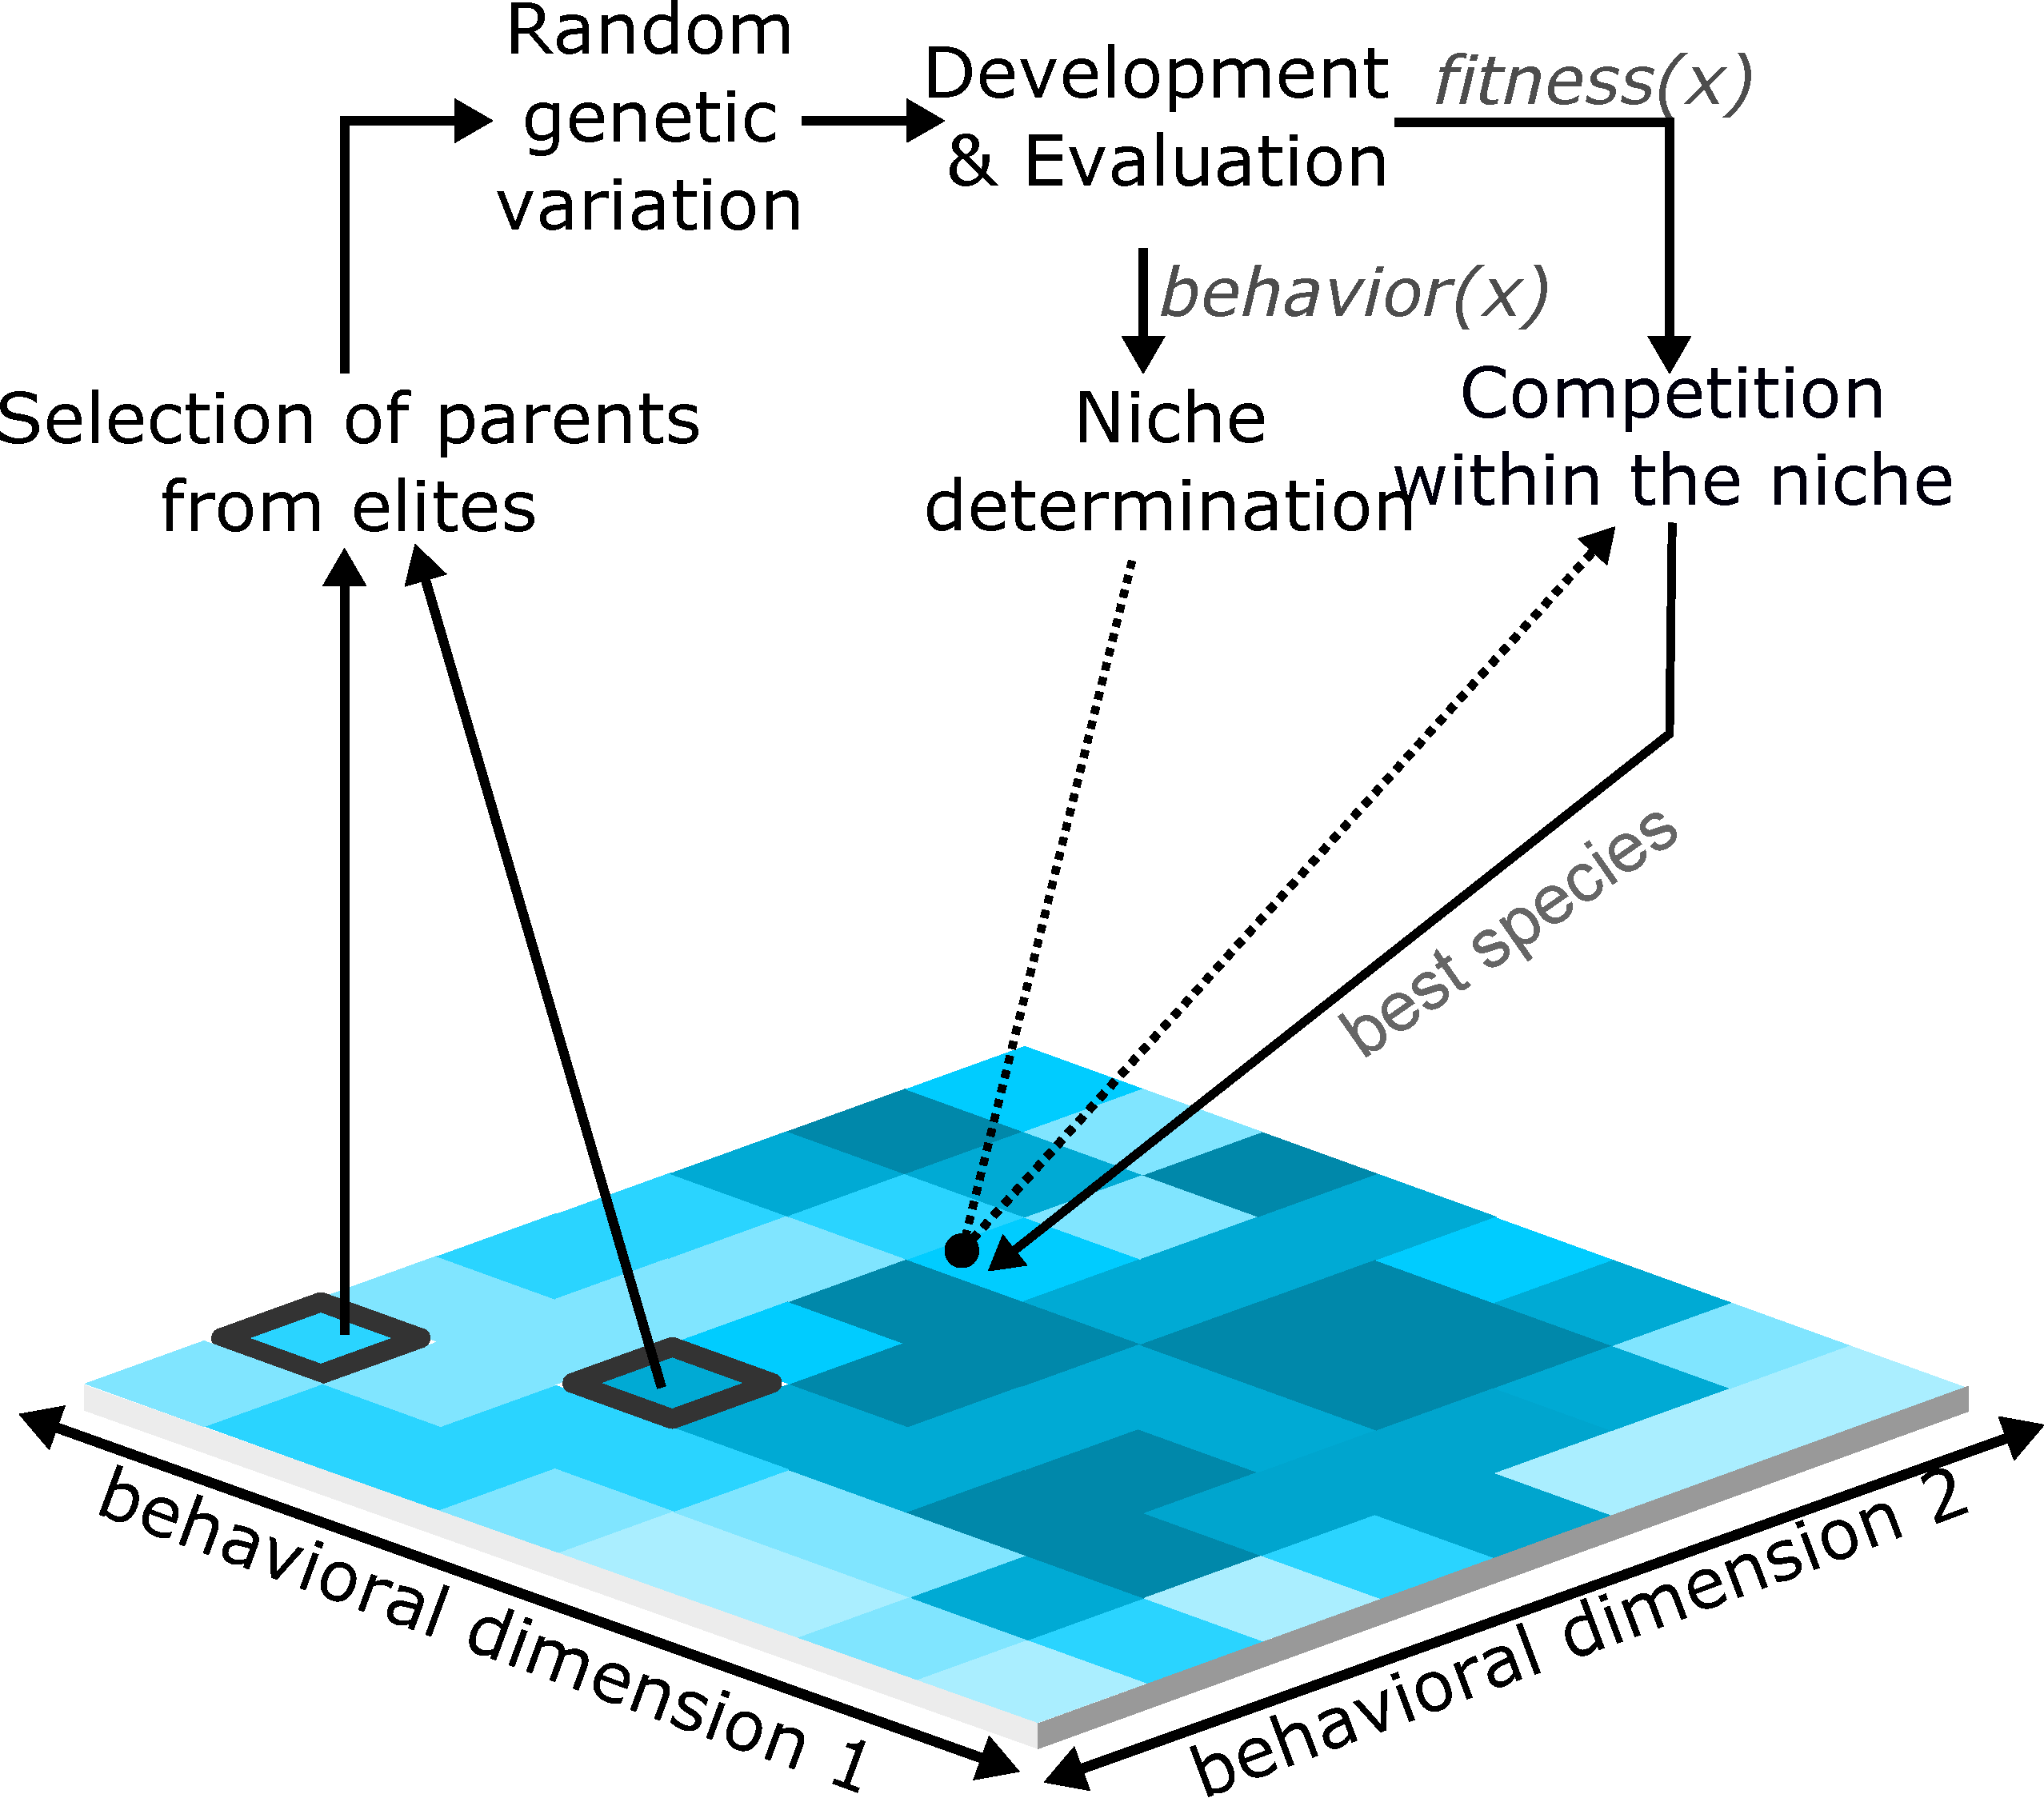
\includegraphics[width=0.4\textwidth]{Bilder/map_elites}
    \caption{MAP-Elites \citep{Mouret_2021}.}
    \label{fig:map-elites}
\end{figure}


\subsection{Multi-Objective Optimization}
The hexapod robot from the example above had as objective to walk forward as fast as possible. However, in real-world situations, robots usually have more than one objective. For example, the robot could not only be required to be fast, but also to minimize its energy consumption. In multi-objective (MO) optimization, there can be $n$ different objectives that should be maximized or minimized, depending on the problem. More formally, the objective is to maximize or minimize the following function: 
\begin{equation}
\label{eq:mo}
\mathbf{y} = f(\mathbf{x})=(f_{1}(\mathbf{x}), f_{2}(\mathbf{x}), \dots, f_{n}(\mathbf{x}))
\end{equation}
where $\mathbf{x}=(x_{1}, x_{2}, \dots, x_{k})\in \mathcal{X}$ is a tuple representing the \textit{decision vector} (solutions), and $\mathbf{y}=(y_{1}, y_{2}, \dots, y_{n})\in \mathcal{Y}$ is the tuple representing the \textit{objective vector}. Therefore, function $f$ maps a $k-\text{dimensional}$ solution to a tuple of $n$ objectives \citep{zitzler1998evolutionary}. To define the region of the solution space where all possible valid solutions can be found, also known as \textit{feasible decision variable space}, the MO optimization problem can be subject to some constraints that every suitable solution has to satisfy \citep{deb2001multiobjective}.

In MO optimization problems, usually there is no solution that is optimal for all objectives, therefore the objectives come as a trade-off. To understand the goal of this method, it is first necessary to understand the concept of \textit{solution dominance}. A solution $x_{1} \in \mathcal{X}$ is said to dominate a solution $x_{2} \in \mathcal{X}$ (or $x_{1}\succ x_{2}$) iff:
\begin{equation}
\label{eq:dom}
\forall i \in \{1, 2, \dots, n\}: f_{i}(x_{1}) \geq f_{i}(x_{2}) \; \wedge \; \exists j \in \{1, 2, \dots, n\}:f_{j}(x_{1}) > f_{j}(x_{2})
\end{equation}
This means that $x_{1}$ dominates over $x_{2}$ if and only if it performs at least as good as $x_{2}$ across all the objectives and strictly higher in at least one objective \citep{janmohamed2023improving}. 

The goal of MO optimization is to find the set of solutions that is not dominated by any other solution in the search space after all objectives have been considered. In other words, it aims at finding all the solutions that cannot be improved in any other objective without worsening its performance in other objectives. The set of all these decision vectors is known as \textit{Pareto-optimal} \citep{zitzler1998evolutionary}. 
In Figure \ref{fig:pf}, there are two Pareto fronts for a bi-objective problem, where both objectives are to be maximized. The solutions on the blue front dominate the solutions from the red Pareto front.
\begin{figure}[H]
    \centering
    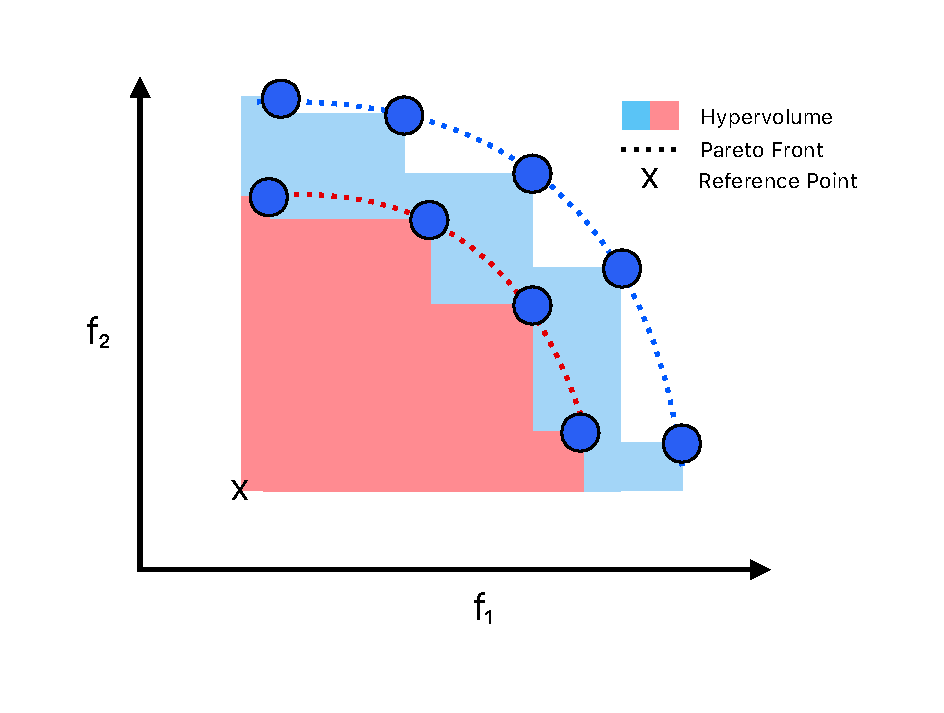
\includegraphics[width=0.5\textwidth]{Bilder/hypervolume}
    \caption{ Pareto fronts and hypervolume.}
    \label{fig:pf}
\end{figure}
To measure the quality of a Pareto front, the \textit{hypervolume} metric can be used. This metric represents the region enclosed by the Pareto front and a given reference point. The advantage of this metric is that a Pareto front that dominates another one, will have a greater hypervolume (as it can be seen in Figure \ref{fig:pf}), while the main disadvantage is that it depends on a reference point that is given by the user. 
Given the $n-\text{dimensional}$ Pareto front $\mathcal{P}=\{(f_{1}(x_{1}), f_{2}(x_{1}), \dots, f_{n}(x_{1})), \dots, (f_{1}(x_{p}), f_{2}(x_{p}, \dots, f_{n}(x_{p}))\}$ with $p$ points (cardinality) and a reference point $\mathbf{r}=(r_{1}, r_{2}, \dots, r_{n})' \in\mathbb{R}^{n}$, its hypervolume $H(\mathcal{P}, \mathbf{r})$ can be expressed as:
\begin{equation}
\label{eq:hypervolume}
H(\mathcal{P}, \mathbf{r})=\lambda(\mathbf{x}\in \mathbb{R}^{n}| \exists \mathbf{s} \in \mathcal{P}, \mathbf{s} \succ \mathbf{x} \succ \mathbf{r})
\end{equation}
Where $\mathbf{x}$ are all the decision vectors in the search space $\mathcal{X}$ and $\lambda$ is the Lebesgue Measure, used to measure the region of a subset in $\mathbb{R}^{n}$ \citep{cao2015using}.


\subsection{Multi-Objective Quality-Diversity Optimization} \label{mome}
Multi-Objective Quality-Diversity (MOQD) optimization involves integrating MO optimization into QD algorithms. For this, the Multi-Objective MAP-Elites (MOME) algorithm is used, which is an extension of the MAP-Elites algorithm but instead of storing single solutions in each cell of the discretized descriptor space, MOME stores Pareto fronts of solutions. The goal of MOQD optimization is to find the Pareto front with the largest hypervolume in each cell. This objective is formalized with the MOQD score:
\begin{equation}
\label{eq:moqd_problem}
\max\limits_{\mathbf{x} \in \mathcal{X}} \sum\limits_{i=1}^m H(\mathcal{P}_i), \ \text{where} \ \forall i, \ \mathcal{P}_i = \mathcal{P}(\{\mathbf{x} \ | \ \mathbf{b}(\mathbf{x}) \in S_i \}). 
\end{equation}
Note that this equation is analogous to Equation \ref{eq:qd_problem}, but adapted to the MO case. 

During each iteration of MOME, a set of cells is chosen, each of which contains a Pareto front. Then a single solution from each Pareto front is selected, copied, mutated and crossed over. Then the objectives and descriptors of the offspring are calculated. These solutions are added to the cells to which their descriptors correspond and the Pareto fronts are updated. The new solution is only added to the Pareto front if it is not strictly dominated by any another solution on the front and any solution that is strictly dominated by the offspring is dropped \citep{pierrot2022multi}. 

The main disadvantage of the solution selection strategy is that it is possible that the continuous objective functions may cause overpopulation of solutions in the Pareto front because of the continuous gaps that can be filled with solutions that only slightly differ in trade-offs. This density in the front can cause a cycle because it is more likely that the exploration happens in more crowded regions, which cause an even denser region, while solutions in sparser regions are more likely to be ignored.
This algorithm also has a disadvantage in its addition mechanism. The Pareto front is of a fixed size, so if a solution is added to a cell that already is at full capacity, it randomly replaces a solution from the cell, which could cause a loss of objective space if the solutions to be replaced are on the border of the front \citep{janmohamed2023improving}.
\begin{figure}[H]
    \centering
    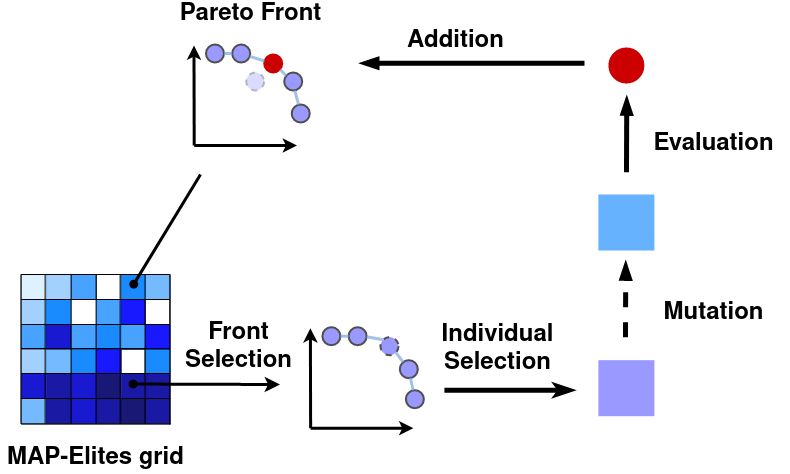
\includegraphics[width=0.5\textwidth]{Bilder/mome}
    \caption{ Multi-Objective MAP-Elites \citep{pierrot2022multi}.}
    \label{fig:mome}
\end{figure}

\subsection{Multi-Objective MAP-Elites with Policy-Gradient Assistance and Crowding-based Exploration (MOME-PGX)}
One way to improve the computational cost of QD algorithms is by improving the exploration strategy. The MOME-PGX algorithm does this by leveraging Policy-Gradient Assistance and Crowding-based Exploration within MOME, which made it between 4.3 and 42 times more data-efficient than MOME \citep{janmohamed2023improving}. A more in-depth description of how these two additions work and how they influence the algorithm can be found in the following subsections.
\begin{figure}[H]
    \centering
    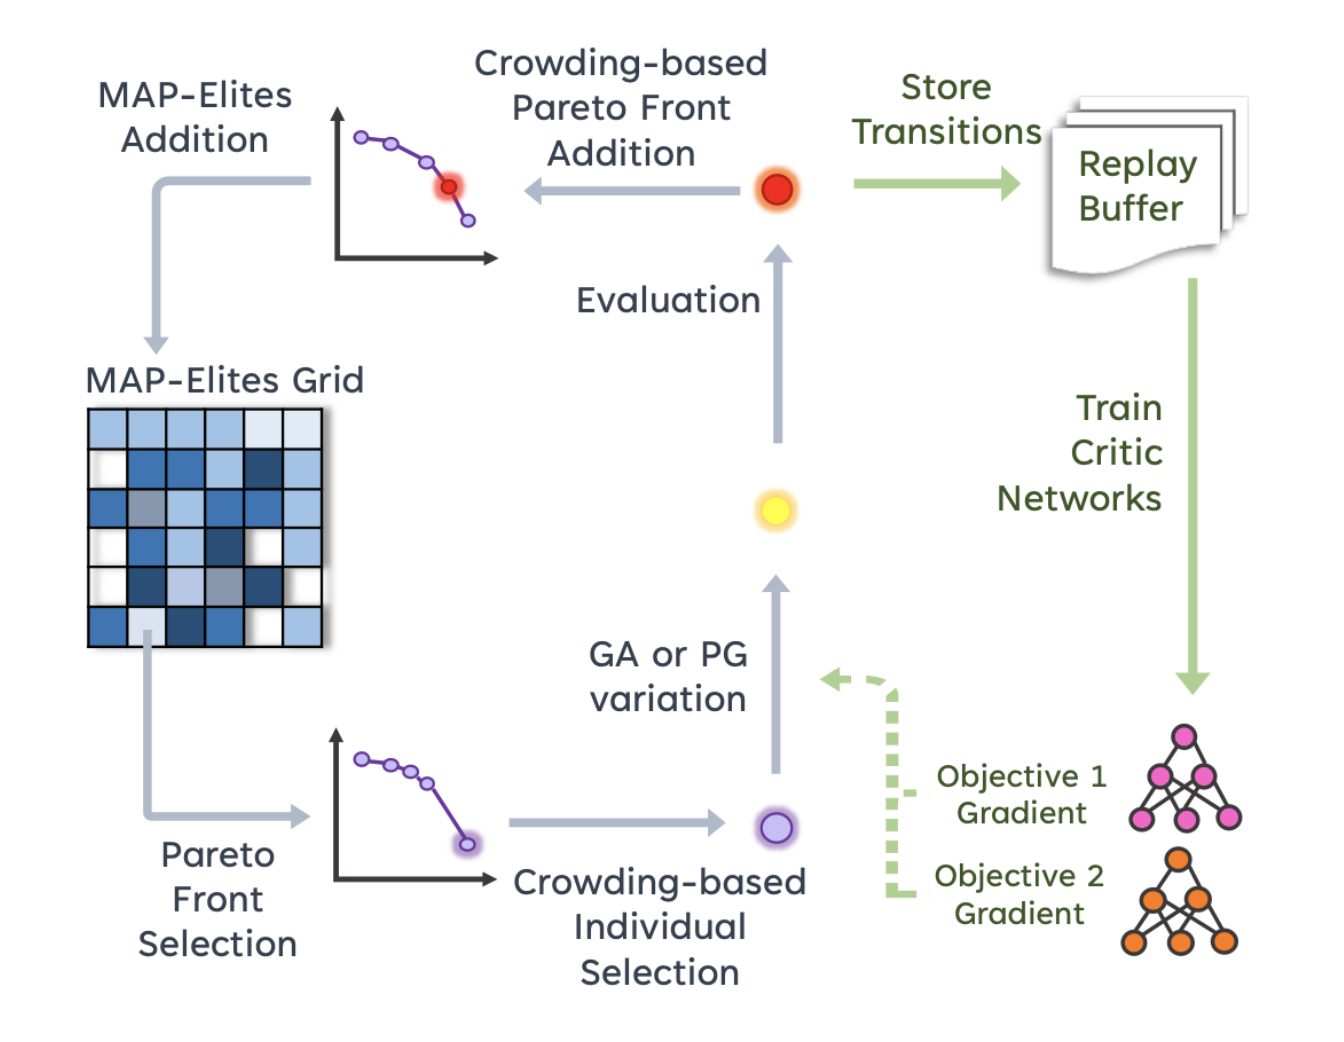
\includegraphics[width=0.5\textwidth]{Bilder/MOME-PGX}
    \caption{ MOME-PGX algorithm \citep{janmohamed2023improving}.}
    \label{fig:momepgx}
\end{figure}

\begin{itemize}
\item \textbf{Policy-Gradient Assistance:} 
\end{itemize}
MOME-PGX uses gradient-based optimization by incorporating the Deep Reinforcement Learning (DRL) algorithm of Twin Delayed Deep Deterministic policy gradient (TD3) \citep{fujimoto2018addressing}, one of the state-of-the-art methods in DRL for robotics. 

First, it is important to understand the basics of DLR. It can be defined as a Markov Decision Process (MDP) because it models the robot's sequential decision making over discrete time-steps $t$. In this field, an agent interacts with the environment and each time-step, it observes the current state $s_t$, and, through a policy $\pi_{\phi}(s)$, chooses an action $a_t$ that leads to the next state $s_{t+1}$ \citep{nilsson2021policy}. \\
The reward $r(s_t, a_t)$ determines how good the action is given the current state. On the other hand, the return is the cumulative sum of weighted rewards from the current state to the goal state:
\begin{equation}
\label{eq:return}
R_t=\sum_{i=t}^{T} \gamma^{i-t}r(s_{i}, a_{i})
\end{equation}
where $T$ is the duration of the whole episode and the discount rate is $0\leq \gamma \leq 1$ which determines the importance of future rewards. A larger $\gamma$ means a lower discounting of future rewards and therefore, a bigger weight on long-term rewards. On the other hand, a smaller $\gamma$ results in a higher discounting of future rewards, giving more importance to short-term rewards \citep{Simonini18}.

To measure the quality of the policy, an objective function $J(x)=\mathbb{E}[R_0]$ is used which is the expected return over the entire episode $T$:
\begin{equation}
\label{eq:obj}
J(x)=\sum_{j=0}^{T} \gamma^{j}r(s_{j}, a_{j})
\end{equation}
Therefore, the goal of DLR is to find a policy that maximizes the objective function $J(x)$. 

In TD3, the goal is to maximize the action-value function $Q^\pi(s, a)=\mathbb{E}[R_t|s,a]$ which captures the expected return of taking an action $a_{t}$ at the state $s_{t}$. This leads to an indirect learning of an actor's policy since maximizing the action-value function, leads to a maximization of the return \citep{nilsson2021policy}. TD3 trains two critics (deep neural networks) with parameters $\theta_1$ and $\theta_2$ by using a replay buffer $\mathcal{B}$ where transition tuples $(s_{t}, a_{t}, r_{t}, s_{t+1})$ are stored. These critics are trained to approximate the action-value function:
\begin{equation}
\label{eq:av}
Q(s_{t}, a_{t})=\mathbb{E}\left[ \sum_{j=t}^{T} \gamma^{j}r(s_{j}, a_{j})\right]
\end{equation}
This is then used to calculate the performance gradient of the policies using deterministic policy gradient:
\begin{equation}
\label{eq:pg}
\nabla_{x_{i}}J_{x_{i}}=\mathbb{E}\left[ \nabla_{x_{i}}\pi_{x_{i}}(s)\nabla_{a}Q_{\theta}(s, a)|_{a=\pi_{x_{i}}(s)}\right],
\end{equation}
This gradient indicates the direction in which the solution $x_i$ should be updated to maximize the reward \citep{janmohamed2023improving}. In order to avoid overestimation, TD3 takes the minimum action-value approximation between the two critics when calculating the update target  \citep{nilsson2021policy}. 

In each iteration of MOME-PGX, half of the solutions are mutated via a genetic algorithm (GA) variation operator and the rest is split into $m$ equal batches, which are then updated using policy-gradients (PG) specific to each objective function. The use of PG mutation operators helps directing solutions to a higher performance across each objective, and the GA operators help maintaining a "divergent search" \citep{janmohamed2023improving}.

\begin{itemize}
\item \textbf{Crowding-based Exploration:} 
\end{itemize}
Another addition of MOME-PGX is the crowding-based selection and replacement strategy, which addresses the main problem with the exploration process of MOME described in section \ref{mome}. The crowding distance corresponds to the average Manhattan distance between a solution and its neighbors, as shown in the left side of Figure \ref{fig:crowding}. During each iteration, a cell is chosen with uniform probability, but the solution is chosen from the Pareto front with a probability proportional to it's crowding distance, so solutions in sparser regions are more likely to be chosen. 

To address the problem of MOME with solutions replacement when the Pareto front is at maximum capacity, MOME-PGX keeps solutions according to their crowding distance: the solutions with biggest crowding distance are kept, while solutions with shorter distance are replaced (right side of Figure \ref{fig:crowding}). This helps providing the greatest variety of trade-offs since the more distant the solutions are in the objective space, the more different trade-off of objectives they have  \citep{janmohamed2023improving}.

\begin{figure}[H]
    \centering
    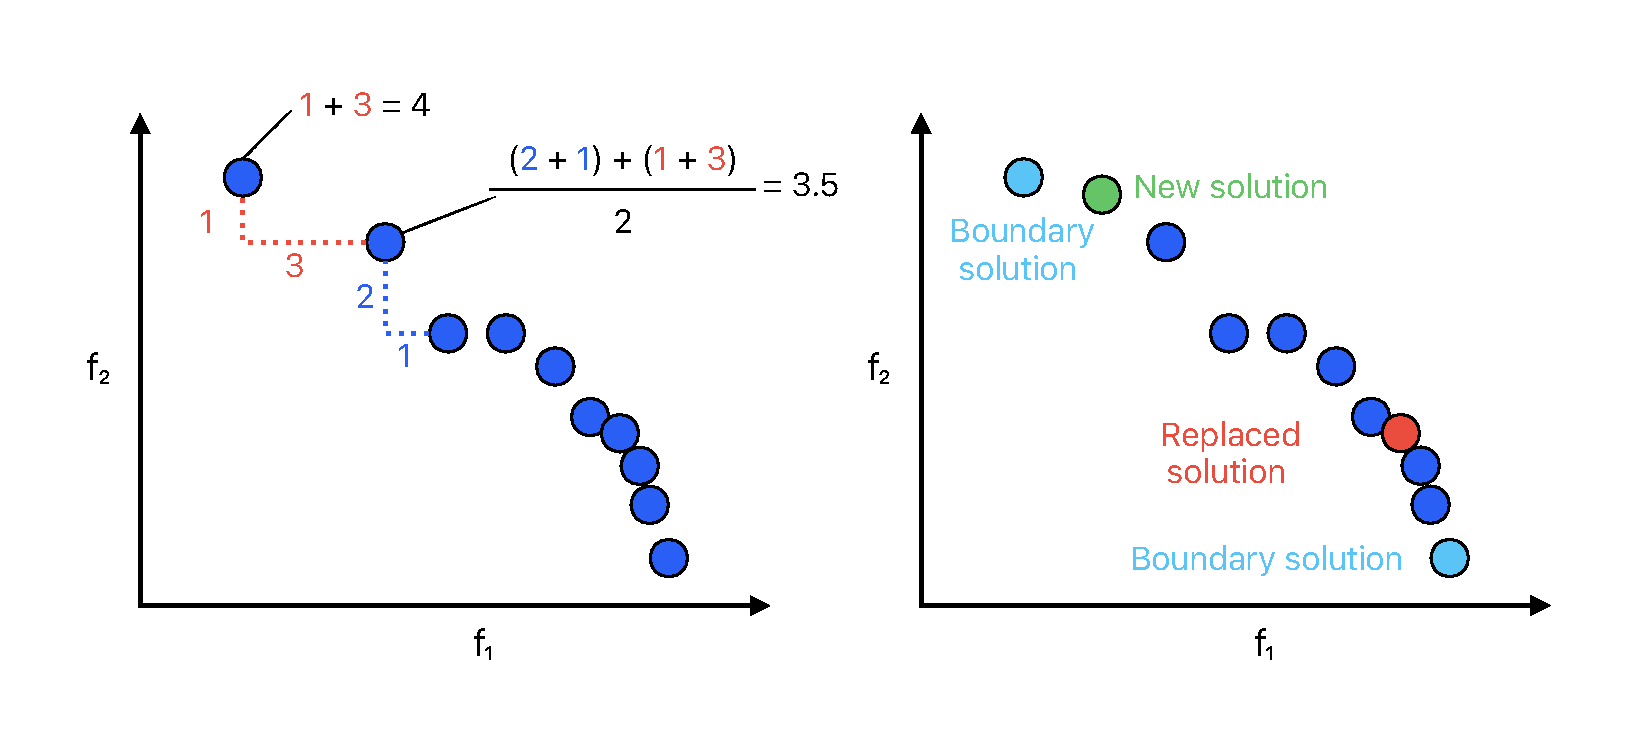
\includegraphics[width=0.85\textwidth]{Bilder/crowding}
    \caption{A Pareto front with two objectives $f_1$ and $f_2$, where the crowding distance is computed (left) and the replacement mechanism is shown (right).}
    \label{fig:crowding}
\end{figure}
\subsection{Map-based Bayesian Optimization Algorithm (M-BOA) for Adaptation} \label{mboa}

\citet{cully2015robots} proposed the Intelligent Trial and Error (IT\&E) algorithm for robotic adaptation using the map generated by the MAP-Elites algorithm. For this, the adaptation step uses a map-based Bayesian optimization algorithm (M-BOA) that trains a Gaussian Process (GP) to model the difference between simulation and reality. 

The adaptation process involves the following steps (the notations are specified in Section \ref{notations}):

\begin{enumerate}
    \item \textbf{Initialization}:
        \begin{itemize}
            \item Initialize the GP model with the behavior-performance map created by MAP-Elites. The GP predicts the performance of behaviors and quantifies uncertainty.
        \end{itemize}
    
    \item \textbf{Selection of Behaviors}:
        \begin{itemize}
            \item Use the Upper Confidence Bound (UCB) acquisition function to select the next behavior to test. The UCB balances exploration (choosing behaviors with high uncertainty) and exploitation (choosing behaviors expected to perform well):
            \begin{equation}
            \label{eq:ucb}
            \chi_{t+1} = \arg \max_\mathbf{x} (\mu_t(\mathbf{x}) + \kappa \sigma_t(\mathbf{x}))
            \end{equation}
            \item Here, \(\mu_t(\mathbf{x})\) is the predicted performance, \(\sigma_t(\mathbf{x})\) is the uncertainty, and \(\kappa\) is a parameter that controls the exploration-exploitation trade-off.
        \end{itemize}
    
    \item \textbf{Testing and Updating}:
        \begin{itemize}
            \item The selected behavior $\chi_{t+1} $ is tested on the physical robot, and its actual performance $\mathbf{P}_{t+1}$ is measured.
            \item The GP model is updated with the new data, adjusting both the mean and variance:
            \begin{equation}
            \label{eq:mean_update}
            \mu_{t+1}(\mathbf{x}) = \mathbf{k}^T \mathbf{K}^{-1} (\mathbf{P}_{1:t+1} - \mathcal{P}(\mathbf{x}_{1:t+1}))
            \end{equation}
            \begin{equation}
            \label{eq:variance_update}
           \sigma_{t+1}^2(\mathbf{x}) = k(\mathbf{x}, \mathbf{x}) - \mathbf{k}^T \mathbf{K}^{-1} \mathbf{k}
            \end{equation}
            \item This GP models the difference between real performance $\mathbf{P}_{1:t+1}$ and the performance from simulation $\mathcal{P}(\mathbf{x}_{1:t+1})$ of all the tested behaviors.
        \end{itemize}
    
    \item \textbf{Stopping Criterion}:
        \begin{itemize}
            \item The adaptation process continues iteratively until the performance of a tested behavior exceeds a predefined threshold relative to the best predicted performance:
            \begin{equation}
            \label{eq:stopping}
            \max(\mathbf{P}_{1:t}) \geq \alpha \max_\mathbf{x} (\mu_t(\mathbf{x}))
            \end{equation}
            \item Typically, \(\alpha\) is set to 0.9, indicating that the search stops when a behavior achieving 90\% of the maximum expected performance is found.
        \end{itemize}
\end{enumerate}

%%%%%%%%%%%%%%%%%%MOTIVATION%%%%%%%%%%%%%%%%%%%%%%%%%%%%%%%%%%%%%%%%%%%
\section{Motivation}
Quality-Diversity algorithms have been successful when providing a diverse set of effective solutions for adaptation. However, this set of solutions could be less useful when the simulation model that it is generated with has important inaccuracies. Therefore, the first research question that this work aims to answer is:
\begin{itemize}
\item To what extent do inaccuracies in the simulation model impact the performance of QD algorithms in finding high-quality solutions?
\end{itemize}
This question explores the robustness of QD algorithms against errors and inaccuracies in the simulation parameters, making it possible to evaluate how sensitive these algorithms are. This is an important aspect to consider when using QD algorithms for real-world scenarios because the simulation models cannot perfectly represent the real-world due to aleatory and epistemic uncertainties, such as friction, contact dynamics, or unknown simulation parameters \citep{choi2021use}. 

To investigate this question, controlled inaccuracies should be systematically introduced to the simulation and the performance of the QD algorithm should be observed. It is expected that the algorithm will find at least one high-performing solution for light inaccuracies and that it will not find any suitable solution for more important inaccuracies. The modifications to the environment include: friction value, obstacles, and restriction of possible ways to reach the goal.

Besides the QD algorithms robustness, this research aims at exploring an approach to improve the model adaptation, which leads to the second research question:

\begin{itemize}
\item Can the model be improved faster and more efficiently by leveraging the exploration behaviors learned during the process?
\end{itemize}
This question is explored by setting up a QD algorithm with primary objectives such as minimizing energy consumption and optimizing distance to a target. These initial objectives help establish a baseline for performance. Then, an exploration criterion is implemented within the MO optimization. This criterion measures the duration of contact between the robot's leg and the object. This approach ensures that the model not only focuses on the primary objective of achieving accurate kicks but also learns from diverse interactions that provide insights into the environmental dynamics, such as friction. The effectiveness of this approach is evaluated by comparing the performance and learning efficiency of models that incorporate this exploration behavior criterion against the baseline. 
%%%%%%%%%%%%%%%%%%DESCRIPTION%%%%%%%%%%%%%%%%%%%%%%%%%%%%%%%%%%%%%%%%%%%

\section{Experiment Design}
\subsection{Baseline}
The evaluations are conducted using the Brax differentiable physics simulator \citep{brax2021github}. The tested robot is a modified version of the Ant model from Brax. It is static except for a single two-jointed leg (see Figure \ref{fig:kicker}). 
\begin{figure}[H]
    \centering
    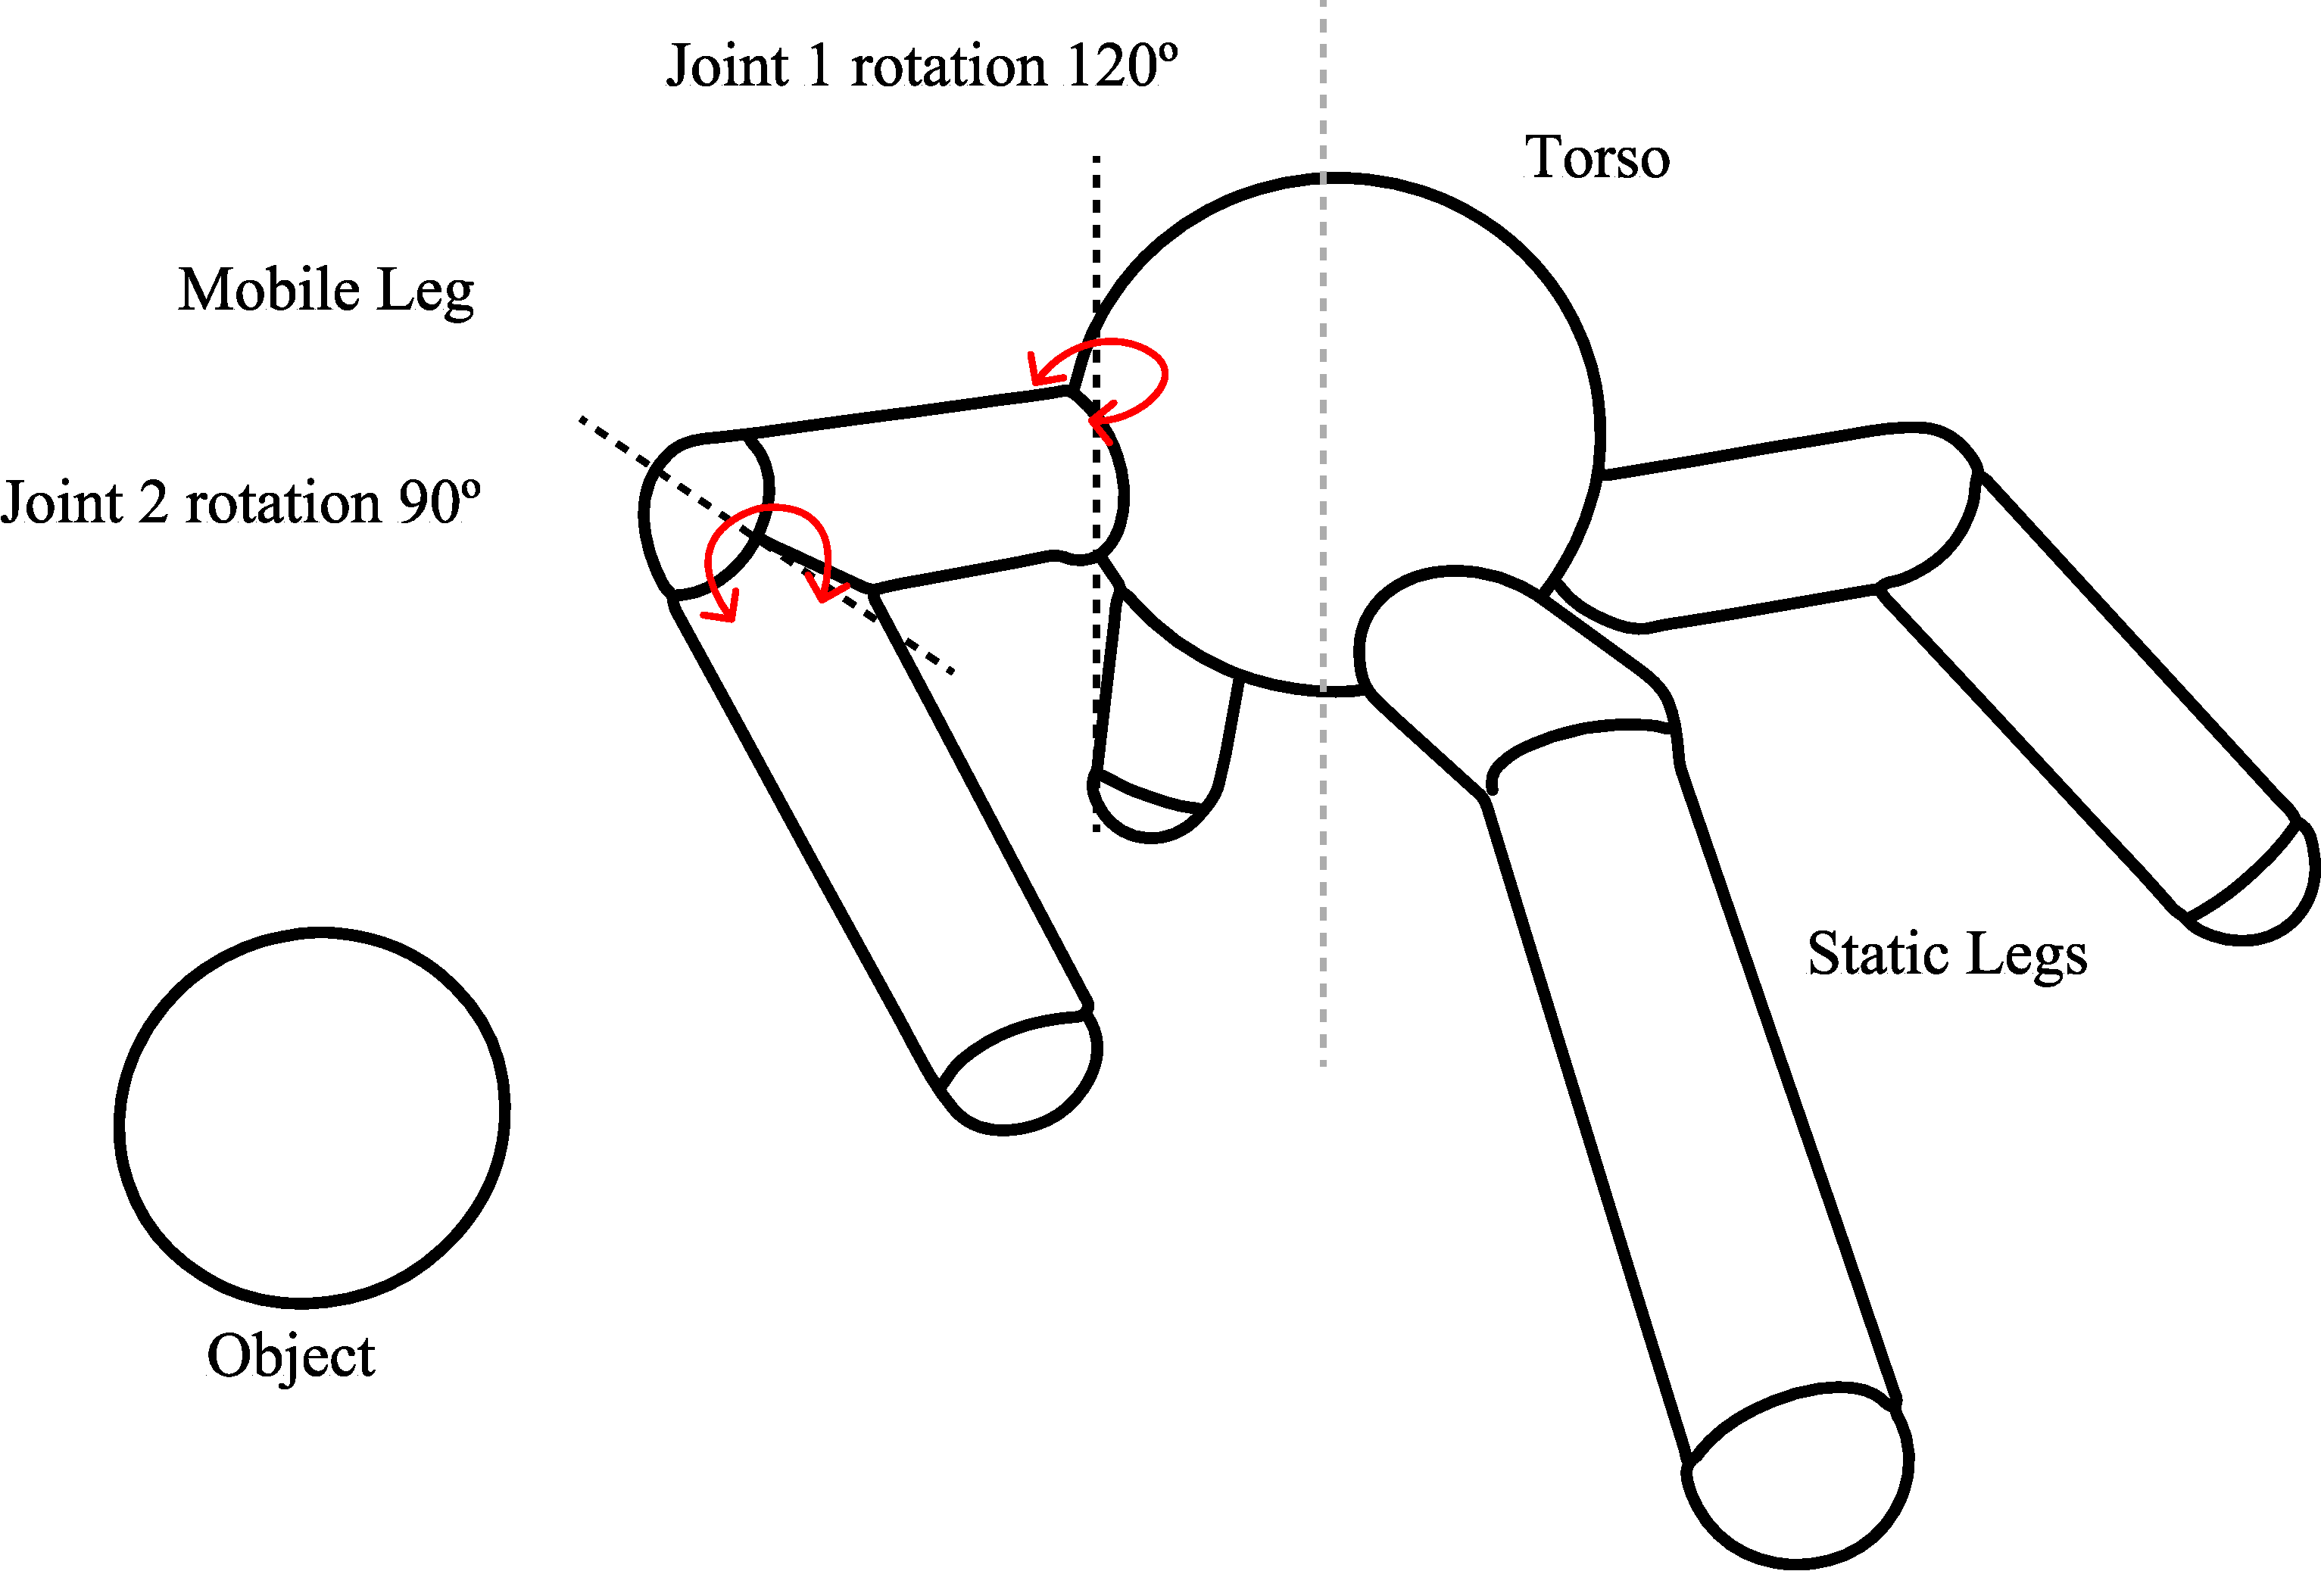
\includegraphics[width=0.6\textwidth]{Bilder/ant_sketch}
    \caption{Diagram of the modified Ant model and an object (ball) to be kicked.}
    \label{fig:kicker}
\end{figure}
The task is to get a set of closed-loop neural-network controllers that allow the robot to kick an object to a target. These controllers control the torque commands $a_t\in [-1, 1]$ of the robot at each time-step $t$ based on the current state $s_t$. 

The action space of the robot is given by the rotation of the hip joint (Joint 1) and the rotation of the ankle joint (Joint 2), therefore an action $(\tau_1, \tau_2)$ corresponds to the torques applied to each joint.

The observation space has a size of $13$ and it consists on:
\begin{itemize}
\item Angles of the joints: 2 angles in total. 
\item Angular velocity of each joint: 2 velocities.
\item $x, y, z$ coordinates of the foot.
\item $x, y, z$ coordinates of the object.
\item $x, y, z$ coordinates of the target. 
\end{itemize}

A neural network with two layers is used and each layer consists of 64 neurons. This corresponds to a solution space of size $5186$.

To characterize the solution space, a behavior descriptor is defined. It corresponds to the average joint workspace ratio during the kick. More formally:

\begin{equation}
\label{eq:bd}
b_i(x) = \frac{1}{K} \sum\limits_{t=k_{begin}}^{k_{end}} b_{i,t} \ \text{for} \ i=1, 2, 
\end{equation}
where $i$ corresponds to the joint, $k_{begin}$ is the time-step when the leg starts contact with the ball (beginning of the kick), $k_{end}$ is the time-step when the contact ends (end of kick),  $K = k_{end} - k_{begin}$ is the kick duration, and $b_{i, t}$ is the workspace ratio at time $t$, which is given by:
\begin{equation}
\label{eq:ratio}
b_{i,t} = \text{clip}\left(\frac{\alpha_{i,t} - \alpha_{i,\text{min}}}{\alpha_{i,\text{max}} - \alpha_{i,\text{min}}}, 0, 1\right),
\end{equation}
where $\alpha_{i,t}$ is the angle of joint $i$ at time $t$, $\alpha_{i,\text{min}}$ is the minimum angle limit of the joint, and $\alpha_{i,\text{max}}$ is the maximum angle limit of the joint. The ratio is clipped between 0 and 1 to avoid any ratio outside these limits, which could happen if the joints experience overshooting due to large actions causing aggressive movements.

The following two objectives are being optimized: accuracy and energy efficiency. If the robot is required to kick the object with the right amount of force for it to stop right at the goal, it would not be appropriate to just consider the position of the object at the most recent moment because that does not provide enough gradient information, causing the robot to fail at learning due to sparse rewards. Therefore, a fitness function that takes into account the position of the ball at all moments is optimal. This approach provides a denser gradient of information, allowing the robot to gradually improve its performance. By integrating this temporal aspect into the fitness function, the robot has a clearer and more continuous signal to follow, making it easier to learn the correct behavior over successive iterations. Therefore, the objective function for accuracy $f_1$ is denoted by:
\begin{equation}
\label{eq:f1}
 f_1=-\sum_{t=1}^{T}\lVert (\mathbf{g} - \mathbf{o}_t) \rVert_2
\end{equation}
where $\mathbf{g}$ is the position vector of the goal, $\mathbf{o}_t$ is the position vector of the object at time $t$, and $\lVert \cdot \rVert_2$ denotes the Euclidean norm. In other words, the accuracy is measured by the negative of the distance of the object to the goal during the entire episode. 

The energy efficiency objective is given by:
\begin{equation}
\label{eq:f2}
 f_2=-\sum_{t=1}^{T} \lVert a_t \rVert_2^2
\end{equation}
In terms of individual rewards at any given time $t$, the accuracy and energy efficiency are expressed in this work as Reward Distance and Reward Control, respectively. Reward Distance is defined as $dist_t=-\lVert \mathbf{g} - \mathbf{o}_t \rVert_2$, and Reward Control is defined as $ctrl_t=-\lVert a_t \rVert_2^2$. 

For generating the repertoire of solutions, it is important to mention some of the used simulation parameters. The general parameters of the environment are shown in Table \ref{tab:environment_configuration}.
\begin{table}[H]
    \centering
    \begin{tabular}{|c|c|}
        \hline
        \textbf{Parameter} & \textbf{Value} \\
        \hline
        Friction & 0.5 \\
        \hline
        Gravity & 9.8 m/s\(^2\) \\
        \hline
        Angular Damping & -0.05 N$\cdot$m$\cdot$s/rad \\
        \hline
        Elasticity & 0.5 Pa \\
        \hline
    \end{tabular}
    \caption{Environment Configuration}
    \label{tab:environment_configuration}
\end{table}

The object's configuration is:

\begin{table}[H]
    \centering
    \begin{tabular}{|c|c|}
        \hline
        \textbf{Parameter} & \textbf{Value} \\
        \hline
        Shape & Sphere \\
        \hline
        Radius & 0.17 m \\
        \hline
        Mass & 0.5 kg \\
        \hline
    \end{tabular}
    \caption{Object Configuration}
    \label{tab:object_configuration}
\end{table}

The goal is configured to spawn at $(2.00, 3.46, 0.00)$ that corresponds to the coordinates in front of the robot, at a distance $r=4.0\ \text{m}$ from its Torso.

An additional experiment is carried out in which the robot is trained in an environment where two walls are placed near the goal to give the robot more ways to reach it (see Figure \ref{fig:kicker_walls}). This repertoire is not tested on different friction coefficients but rather to see how the adaptation behaves when one way of reaching the goal is not available. 

See Appendix \ref{appendix:params} for the complete training parameters and Appendix \ref{appendix:envs} for a visualization of the environments.
\begin{figure}[H]
    \centering
    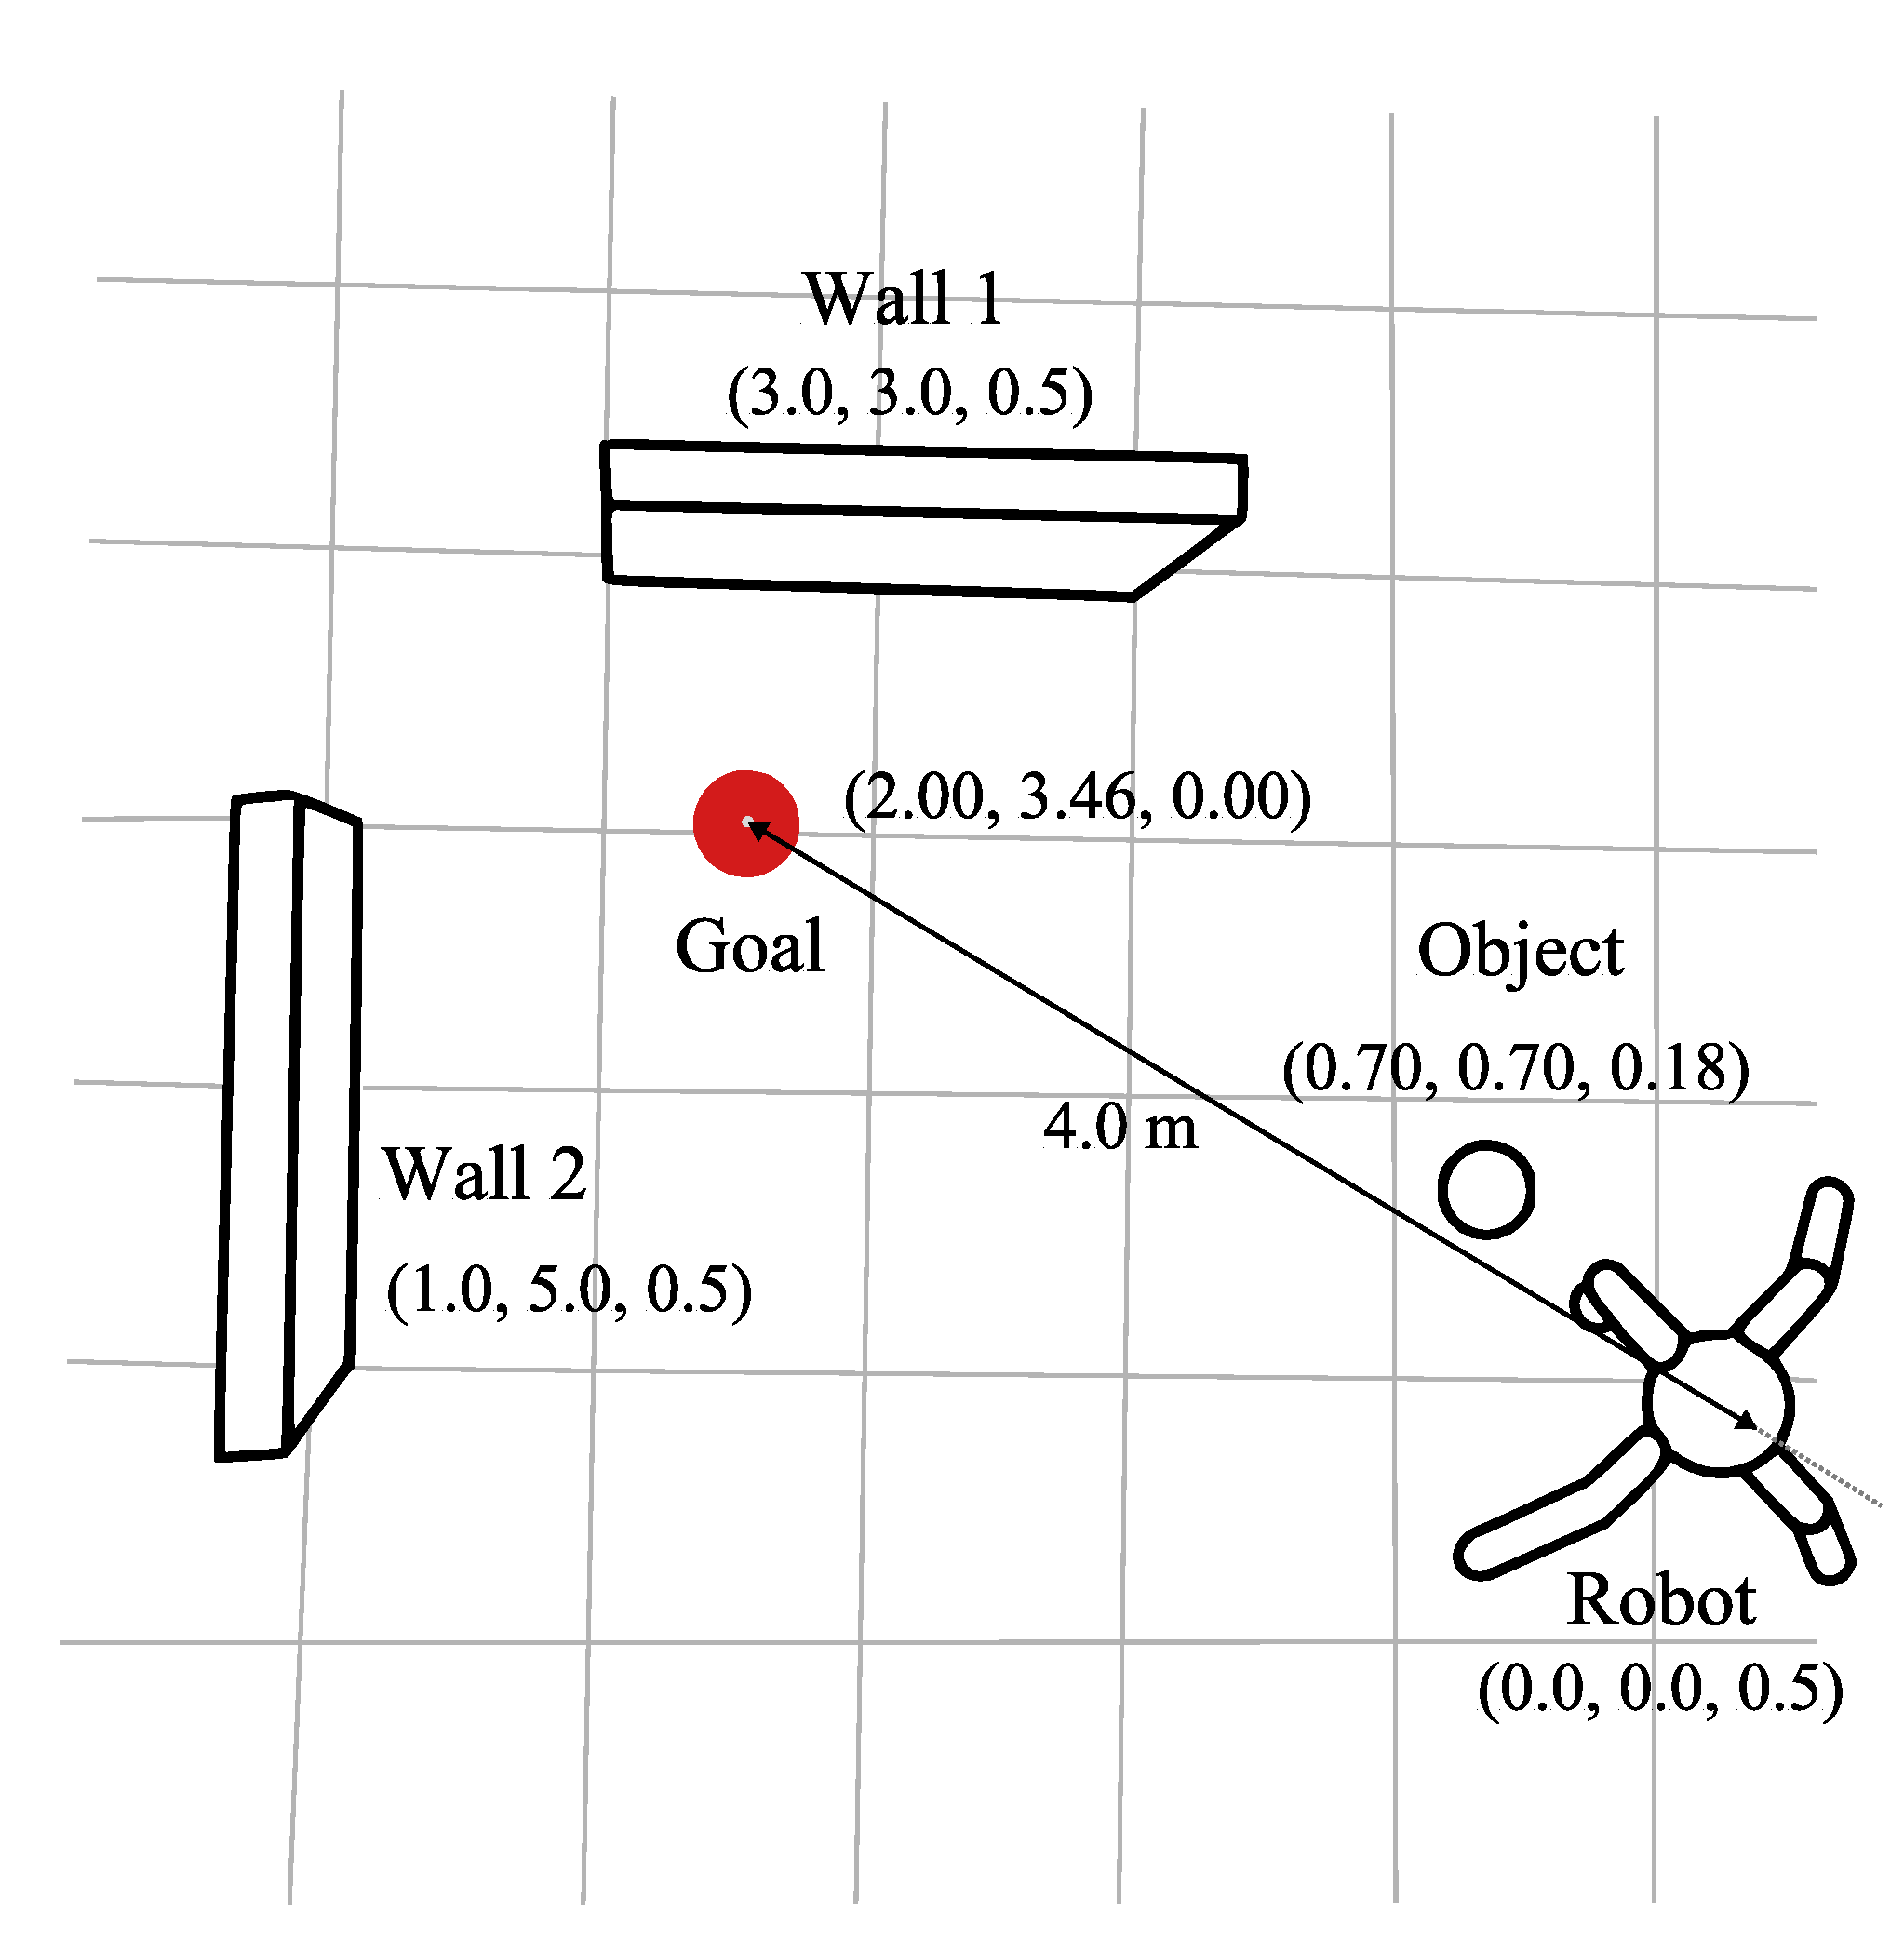
\includegraphics[width=0.6\textwidth]{Bilder/walls}
    \caption{Position of elements in the environment with walls.}
    \label{fig:kicker_walls}
\end{figure}
\subsection{Adaptation}
\subsubsection{Notations}\label{notations}
\begin{itemize}[label={$\bullet$}]
    \item $\alpha$: Threshold parameter that determines the minimum acceptable performance (scalar).
    \item $\kappa$: Exploration-exploitation parameter (scalar).
    \item $\mathcal{X}$: Behavior descriptor map generated by MOME-PGX (associative table).
    \item $\mathbf{x}$: A behavior from the behavior descriptor map (vector).
    \item $\boldsymbol{\chi}$: A behavior that has been tested in the robot (vector).
    \item $\mathcal{P}$: Performance map generated by MOME-PGX (associative table).
    \item $\mathcal{C}$: Controller map generated by MOME-PGX (stores genotypes) (associative table).
    \item $\mathcal{P}(\mathbf{x})$: Max performance at $\mathbf{x}$ from the simulation (scalar).
    \item $\mathcal{C}(\mathbf{x})$: Controller currently stored in $\mathbf{x}$ (vector).
    \item $\boldsymbol{\chi}_{1:t}$: All previously tested behavior descriptors at time $t$ (vector of vectors).
    \item $\mathbf{P}_{1:t}$: Performance in the unknown environment of all the solutions tested on the robot up to time $t$ (vector).
    \item $\mathcal{P}(\boldsymbol{\chi}_{1:t})$: Performance from the simulation for all the solutions tested on the robot up to time $t$ (vector).
    \item $f()$: Simulation-reality offset function (unknown by the algorithm) (function).
    \item $\sigma_{\text{noise}}^2$: Kernel noise (scalar).
    \item $k(\mathbf{x}, \mathbf{x})$: Kernel function (function).
    \item $\mathbf{K}$: Kernel matrix (matrix).
    \item $\mathbf{k}$: Kernel vector (vector).
    \item $\mu_t(\mathbf{x})$: Predicted offset for $\mathbf{x}$ (i.e. the mean of the Gaussian process) (function).
    \item $\mu_t'(\mathbf{x})$: Predicted performance for $\mathbf{x}$ (i.e. the corrected mean) (function).
    \item $\sigma_t^2(\mathbf{x})$: Standard deviation for $\mathbf{x}$ in the Gaussian process (function).
\end{itemize}
\subsubsection{Algorithm}
After generating the repertoire of solutions, the robot is placed in an unknown environment with the goal to efficiently look for the best solution in the repertoire. For this, a Bayesian optimization algorithm similar to M-BOA (Section \ref{mboa}) is used, where the difference $f(\mathbf{x})$ between reality and simulation is modeled, taking into account prior knowledge from the simulation. 

MOME-PGX generates the descriptor map $\mathcal{X}$, the genotype or controller map $\mathcal{C}$, and the fitness or performance map $\mathcal{P}$. The performance map contains the fitnesses for both objectives, but for sake of simplicity, in this work the accuracy objective is considered the main objective and is therefore used for the optimization during the adaptation. 

As shown in Algorithm \ref{alg:mboa-imp}, the initial data point evaluated is the best performing solution from the simulation and then the next indices are selected using the Upper Confidence Bound acquisition function, where $\kappa$ is initially set to $1$ to encourage exploitation. If the performance achieved is greater than a threshold, $\kappa$ is set to $0.03$ to test nearby solutions. The threshold is $90\%$ of the performance in the simulation and is defined by setting $\alpha=0.9$. This approach allows the algorithm to look for potentially better solutions near a solution that is already known to perform well.
\begin{algorithm}[H]
\caption{Bayesian Optimization for Adaptation}\label{alg:mboa-imp}
\begin{algorithmic}
\Require Performance, controller, and descriptor maps ($\mathcal{P}$, $\mathcal{C}$, $\mathcal{X}$) from MOME-PGX \State $\forall \mathbf{x} \in \mathcal{X}$:
    \State \hspace{1em} $\kappa \gets 1$ \Comment{Encourage exploration}
    \State \hspace{1em} $\chi_{1} \gets \arg\max_{\mathbf{x}} (\mathcal{P}(\mathbf{x}))$ \Comment{Index of the best performance in the simulation}
    \State \hspace{1em} $P_{1} \gets$ performance(robot\_reality$(\mathcal{C}(\chi_{1}))$) \Comment{Test in reality}
    \State \hspace{1em} $N \gets 50$ \Comment{Number of iterations}
\For{$t \gets 0$ to \text{N}-1}
\If{$P_{t+1} > (\max \mathcal{P}(\mathbf{x})-\min \mathcal{P}(\mathbf{x}))*\alpha + \min \mathcal{P}(\mathbf{x})$} 
    \State $k \gets 0.03$ \Comment{Encourage exploitation}
\EndIf
\State $P(f(\mathbf{x}) \mid \mathbf{P}_{1:t+1}, \mathbf{x}) = \mathcal{N}(\mu_{t+1}(\mathbf{x}), \sigma_{t+1}^2(\mathbf{x}))$\Comment{Update Gaussian Process}
\State $\mu_{t+1}'(\mathbf{x}) \gets \mathcal{P}(\mathbf{x}) + \mu_{t+1}(\mathbf{x})$ \Comment{Include prior knowledge in the mean}
\State $\chi_{t+2} \leftarrow \arg\max_{\mathbf{x}}(\mu_{t+1}'(\mathbf{x}) + \kappa \sigma_{t+1}(\mathbf{x}))$
\Comment{Select next index}
    \State $P_{t+2} \leftarrow \text{performance}(\text{robot\_reality}(C(\chi_{t+1})))$
\State \text{where}
    \State $\mu_{t+1}(\mathbf{x}) = \mathbf{k}^T \mathbf{K}^{-1} (\mathbf{P}_{1:t+1} - \mathcal{P}(\mathbf{x}_{1:t+1}))$
    \State $\sigma_{t+1}^2(\mathbf{x}) = k(\mathbf{x}, \mathbf{x}) - \mathbf{k}^T \mathbf{K}^{-1} \mathbf{k}$
    \State $\mathbf{K} = 
    \begin{bmatrix}
        k(\chi_1, \chi_1) & \cdots & k(\chi_1, \chi_{t+1}) \\
        \vdots & \ddots & \vdots \\
        k(\chi_{t+1}, \chi_1) & \cdots & k(\chi_{t+1}, \chi_{t+1})
    \end{bmatrix}
    + \sigma_{\text{noise}}^2 \mathbf{I}$
    \State $\mathbf{k} = 
    \begin{bmatrix}
        k(\mathbf{x}, \chi_1) & k(\mathbf{x}, \chi_2) & \cdots & k(\mathbf{x}, \chi_{t+1})
    \end{bmatrix}^T$

\EndFor
\end{algorithmic}
\end{algorithm}
The observations of the Gaussian Process are of the form $\left\{ \chi_n, P_n - \mathcal{P}(\chi_n) \right\}_{n=1}^{N}$, with $P_n - \mathcal{P}(\chi_n) \sim \mathcal{N}(f(\mathbf{x}_n), \nu)$ and $\nu$ is the variance of the noise.

Similar to M-BOA, the Matérn kernel is used for its generality and flexibility, including the Squared Exponential as a special case, and its ability to control the distance at which effects become nearly zero ($\rho$) and the rate of decrease ($\nu$). The parameters used are $\nu=5/2$ and $\rho=0.8$, and some noise is added $\sigma_{\text{noise}}^2=0.001$ to improve the robustness to noisy observations.

In the first iteration of the algorithm, the GP is fitted with a single point, which is used as initialization of the model and does not provide any valuable information. Normally, with only one point there is no way to estimate the shape of the function because the model has no information about variability or the relationship between different points in the input space. However, in this algorithm, the prior knowledge of the performance is included in the predicted mean, which helps guide the next point selection. 




\subsection{Simulation Inaccuracies}
To test the utility of QD algorithms for adaptation after introduction of simulation inaccuracies, the following changes to the environment are made for the robot trained without the walls:
\begin{itemize}
\item Evaluation with different friction values: The robot is tested in environments with friction coefficients in the range [0, 0.9], at 0.1 step.
\item Evaluation with obstacles of different heights between the object and the goal: Horizontal bodies that act as barriers between the goal and the object are placed at a distance of $1.0\ \text{m}$ from the objects original position and their height varied from $0.01\ \text{m}$ to $0.07\ \text{m}$ at a step of $0.01\ \text{m}$.
\end{itemize} 
For the robot trained with the two walls, the changes consist of testing it with only one of the walls.
It is important to highlight that these inaccuracies are tested one by one while keeping the others the same as the baseline.

\subsection{Exploration Behavior}
To evaluate the model efficiency improvement, a diversity criterion based on the duration of contact between the robot's leg and the object is introduced. This criterion is considered useful for exploring different environmental dynamics, such as friction, which can vary in reality and affect the robot's performance. The chosen criterion measures the duration for which the leg maintains contact with the object during an episode. This helps explore the friction between the object and the ground, providing insights into how different friction values affect the interaction and movement of the object. Prolonged or varied contact durations can help the robot learn how different interaction strategies (e.g., soft vs. hard kicks) affect the object. This understanding allows the robot to adjust its actions based on the specific dynamics of the new environment. This criterion is included as a behavior descriptor on the $x$ axis of the grid, and is mapped to [0, 1] using a sigmoid function. Let \( N \) be the number of time-steps that the leg is in contact with the ball:
\begin{equation}
\label{eq:contact}
N = \sum\limits_{t=1}^{T} b_{1,t},
\end{equation}
where \( b_{1,t} = 1 \) when the leg is in contact with the ball at time-step \( t \) and 0 otherwise.

Then, the first dimension of the behavior descriptor is:
\begin{equation}
\label{eq:sigmoid}
b_1(x) = \frac{1}{1 + e^{-0.1\left(N - 50\right)}}
\end{equation}

The other dimension of the behavior descriptor is modified to be the average of joint ratios:
\begin{equation}
\label{eq:desc1}
b_2(x) = \frac{1}{N} \sum\limits_{t \in \mathcal{T}} b_{2,t}
\end{equation}
where \( \mathcal{T} \) is the set of time-steps when \( b_{1,t} = 1 \), and \( b_{2,t} \) is the average workspace ratios of the joints at time-step \( t \):
\begin{equation}
\label{eq:desc2}
b_{2,t} = \frac{1}{2} \sum\limits_{i=1}^{2} \left( \frac{\alpha_{i,t} - \alpha_{i,\text{min}}}{\alpha_{i,\text{max}} - \alpha_{i,\text{min}}} \right) \text{for } i=1,2,
\end{equation}
where the notation is the same as in Equation \ref{eq:ratio}.

The sigmoid function from Equation \ref{eq:sigmoid} is chosen after testing several variations with different parameters that map different domains to the interval \([0, 1]\). A value of \(0.1\) ensures that the function is sufficiently sensitive to the variations of the contact time-steps, providing more detail about the interaction. The term \(-50\) shifts the function to the right, so that the range starts at 0 when the domain is close to 0, since the contact time-steps are always positive.

\subsection{Metrics} \label{metrics}

To evaluate the performance of a solution, the fitness function (Equation \ref{eq:f1}) is used. A solution is considered optimal if it achieves a performance of $90\%$ or more of the performance of the best solution from the simulation. This threshold has been used in other studies \citep{cully2015robots} to ensure the adequate functionality of the robot. However, having a threshold that depends on the performance of the simulation is not ideal if the best solution from the simulation is suboptimal. In such cases, even if a solution achieves 90\% of the performance, it would be a useless solution. In this work, the repertoires are ensured to have an optimal solution able to solve the task by accurately kicking the ball to the target. It is also experimentally confirmed that a 90\% of this performance is enough for the ball to still reach the goal. 

The MOQD score (described in Section \ref{mome}) is used to determine how leveraging the additional exploration criterion affects the MOQD optimization during training.

\section{Experimental Results} \label{results} 

\subsection{Baseline Without Walls}

After training the robot for 200 iterations, the solution with highest accuracy $f_1$ reached a maximum Reward Distance of $-0.170$ and a minimum Reward Control of $-0.152$ (Figure \ref{fig:baseline_best_sol_metrics}), resulting in total fitness values of $f_1=-372.831$ and $f_2=-1.283$. 

\begin{figure}[H]
    \centering
    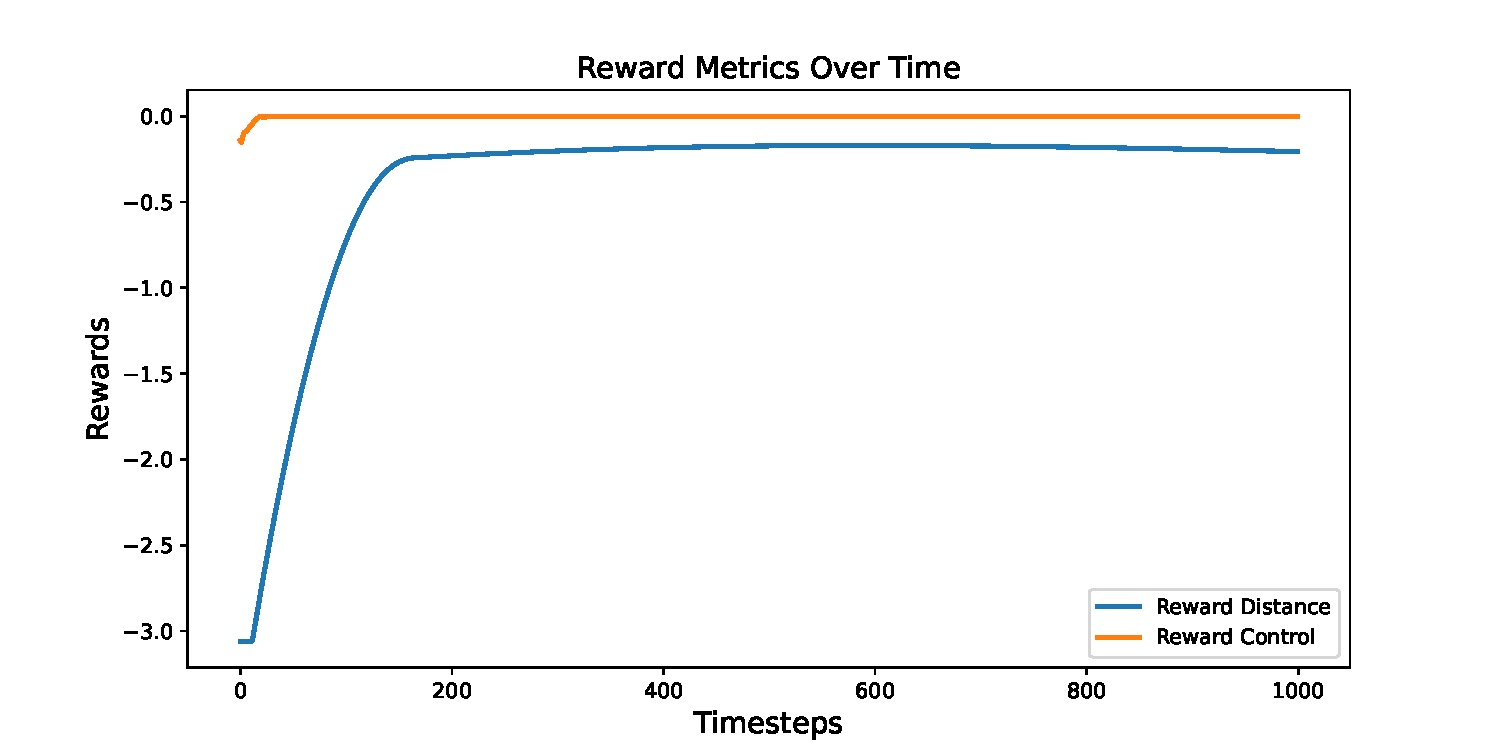
\includegraphics[width=0.9\textwidth]{Bilder/reward_metrics}
    \caption{Rewards over time of the best solution found for the baseline environment without walls, where each line represents an individual reward at a time $t$.}
    \label{fig:baseline_best_sol_metrics}
\end{figure}


The global Pareto front is shown on the leftmost part of Figure \ref{fig:episode_fitness_bs_baseline}, where the colors are assigned based on their respective centroids and are used to identify solutions in the MAP-Elites Grid (Voronoi diagram in the middle). The black markers indicate the solutions that are part of the global Pareto front. The MAP-Elites Grid with the hypervolume of the Pereto front of each cell is on the right.

\begin{figure}[H]
    \centering
    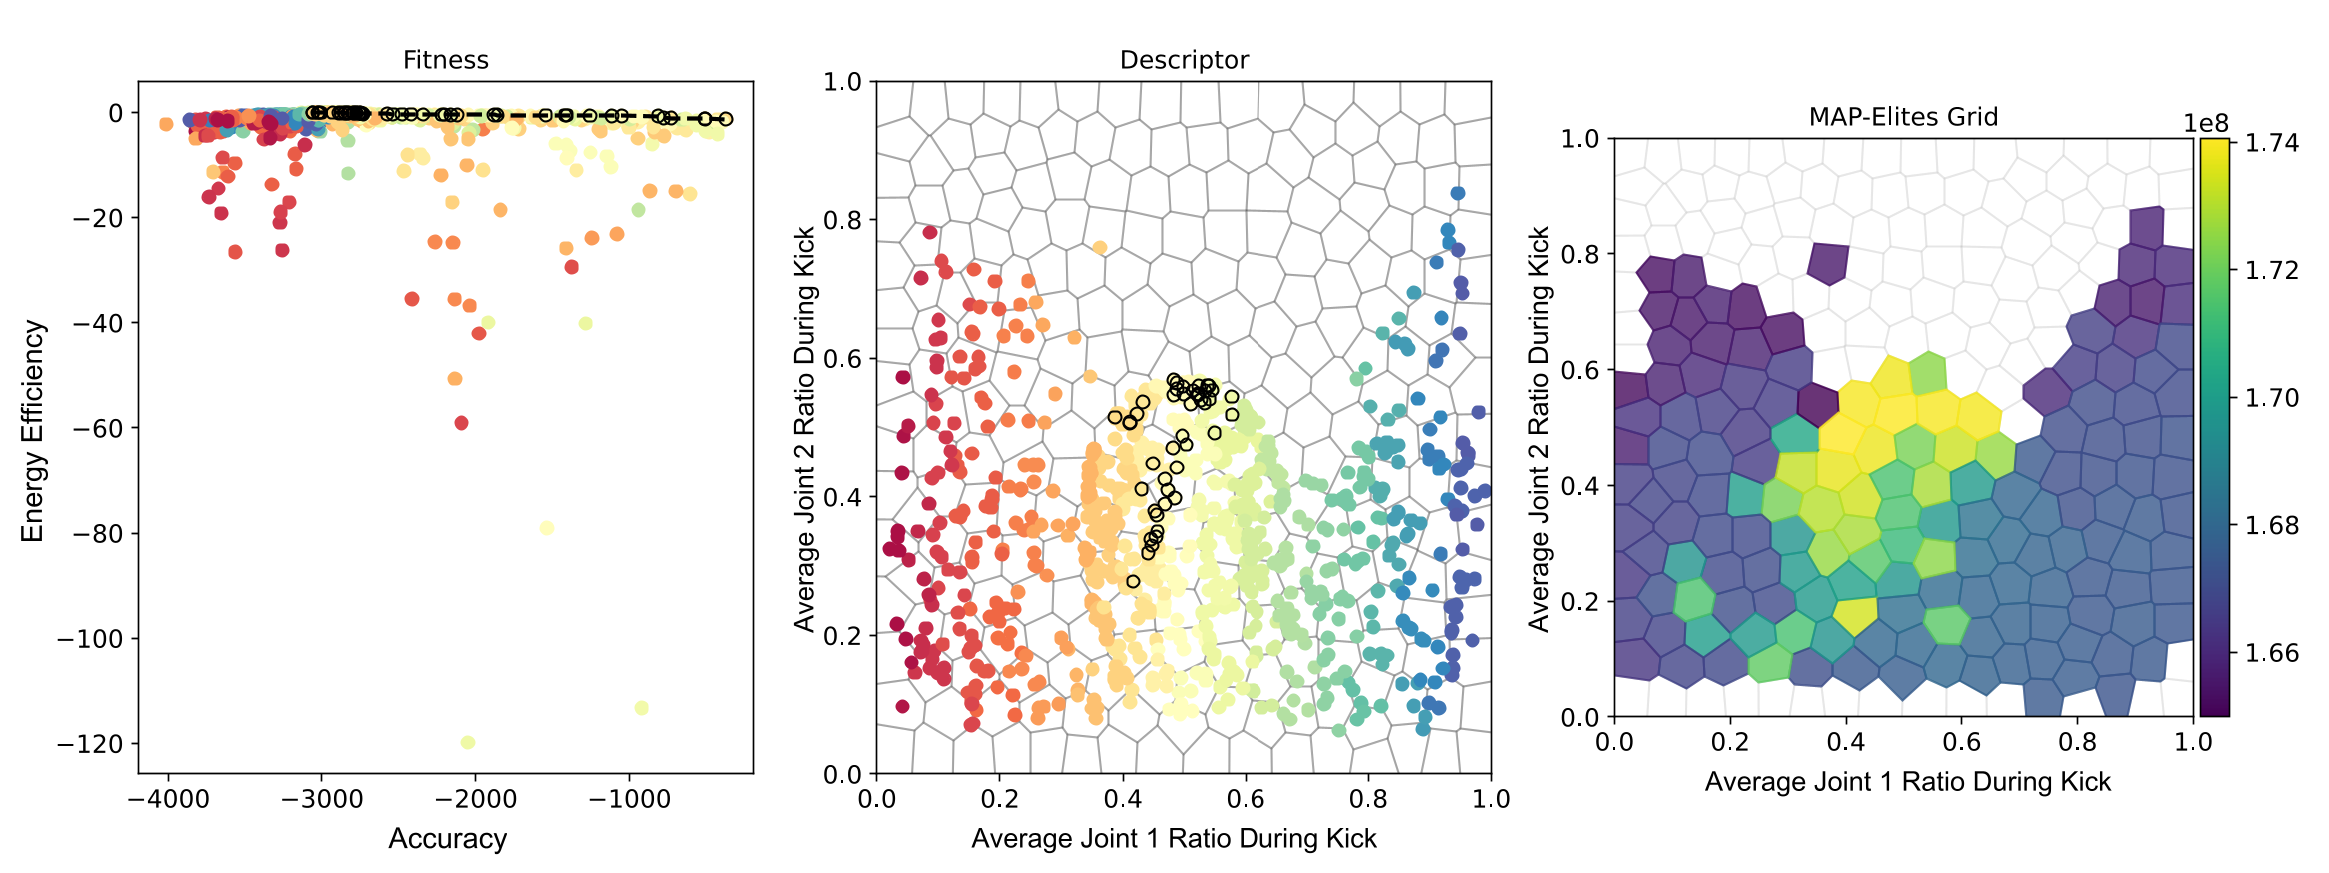
\includegraphics[width=1.0\textwidth]{Bilder/repertoire_baseline_200-flat_}
    \caption{Repertoire generated for the environment without walls: Global Pareto front (left); behavior space, with black circles marking the global Pareto front solutions (middle); MAP-Elites grid, with color intensity representing the hypervolume of the Pareto front in each cell (rigth).}
    \label{fig:episode_fitness_bs_baseline}
\end{figure}
The total coverage is 60.94\%. This U-shaped distribution of populated cells can be explained by the mechanics of the robot’s movement when kicking the ball. When kicking it in a straight line, which corresponds to approximately 50\% of the range of the first joint, the kick ends after the robot used approximately 60\% of the range of its second joint. This results in no more solutions found beyond this range. The robot can also kick diagonally, from the side, or roll the ball from above. In such cases, the first joint’s ranges fall outside the middle values, and the second joint can use more than 60\% of its ratio because it can be fully extended and still make contact with the ball.


The MOQD score and coverage evolutions during training are shown in Figure \ref{fig:scores_evol_baseline}. The initial phase shows that there is a rapid increase in the MOQD score and coverage, indicating that the initial training phase is highly effective in discovering diverse and high-quality solutions. Then, both metrics continue to rise but at a slightly slower rate compared to the initial phase, which suggests that although the training process is still discovering new and better solutions, the rate of improvement is slowing down. Finally, the MOQD score and coverage continue to increase at gradual pace, which suggests that the algorithm finds fewer new solutions. Therefore, training it with more iterations is less probable to lead to any significant improvement. The final MOQD score is $2.6\times 10^{10}$.
\begin{figure}[h]
    \centering
    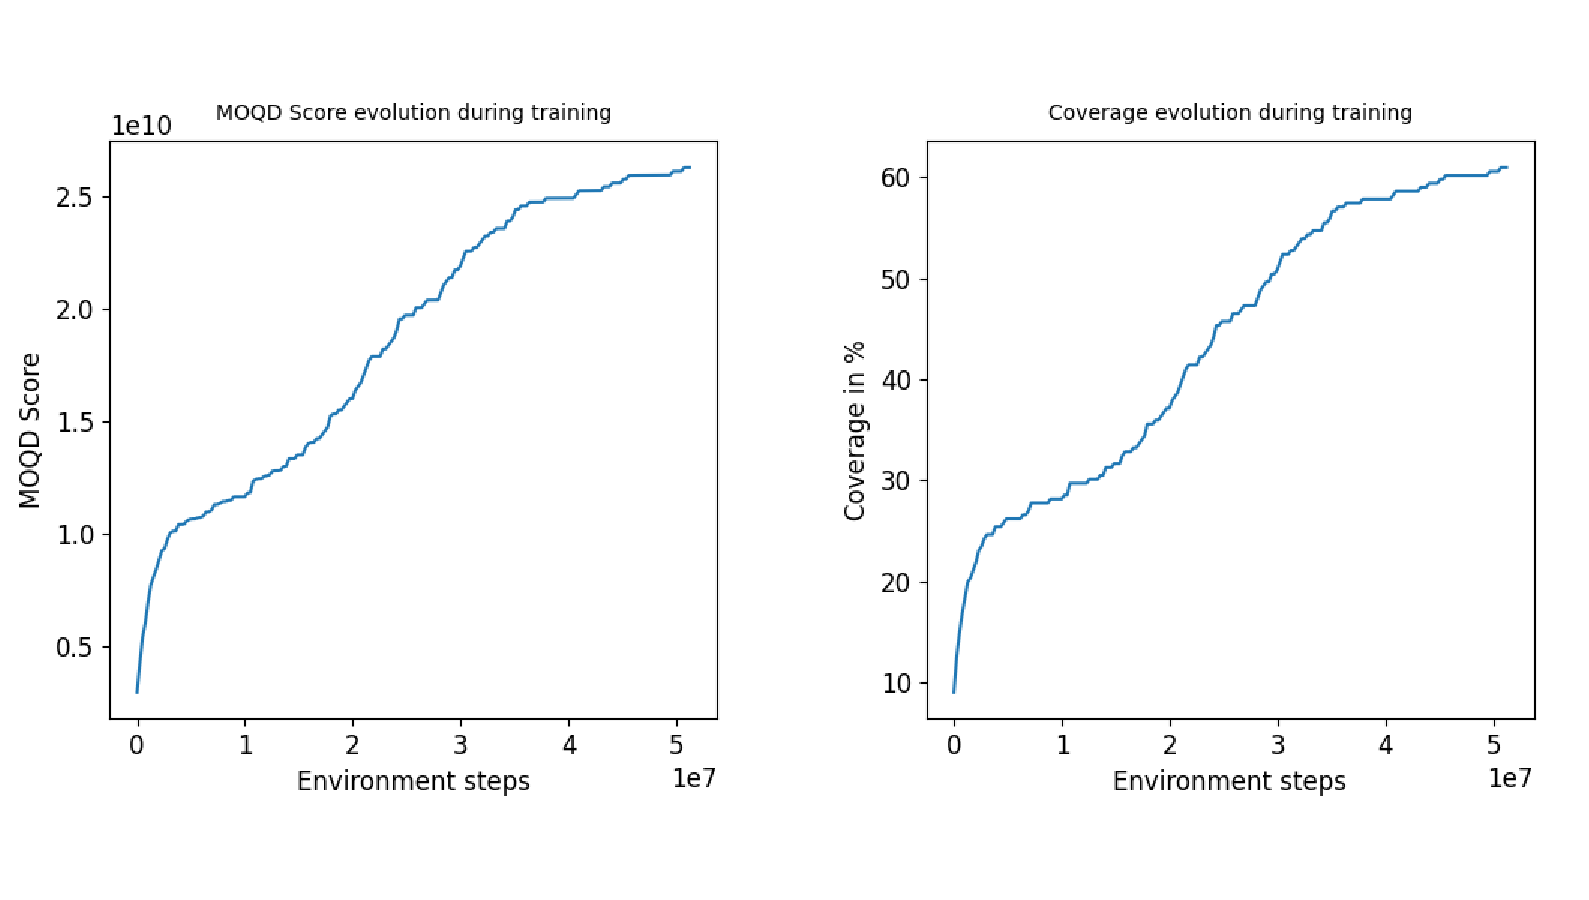
\includegraphics[width=0.9\textwidth]{Bilder/scores_evolution}
    \caption{Scores evolution during training.}
    \label{fig:scores_evol_baseline}
\end{figure}

\subsection{Baseline With Walls}
The robot is also trained in the environment with two walls to give it more ways of achieving the goal, as can be seen in Figure \ref{fig:kicker_walls}. Besides the two walls, all other environment parameters are kept the same as the baseline environment without them. Similarly, the same training parameters are used and the generated repertoire is shown in Figure \ref{fig:episode_fitness_bs_baseline_walls}.
\begin{figure}[H]
    \centering
    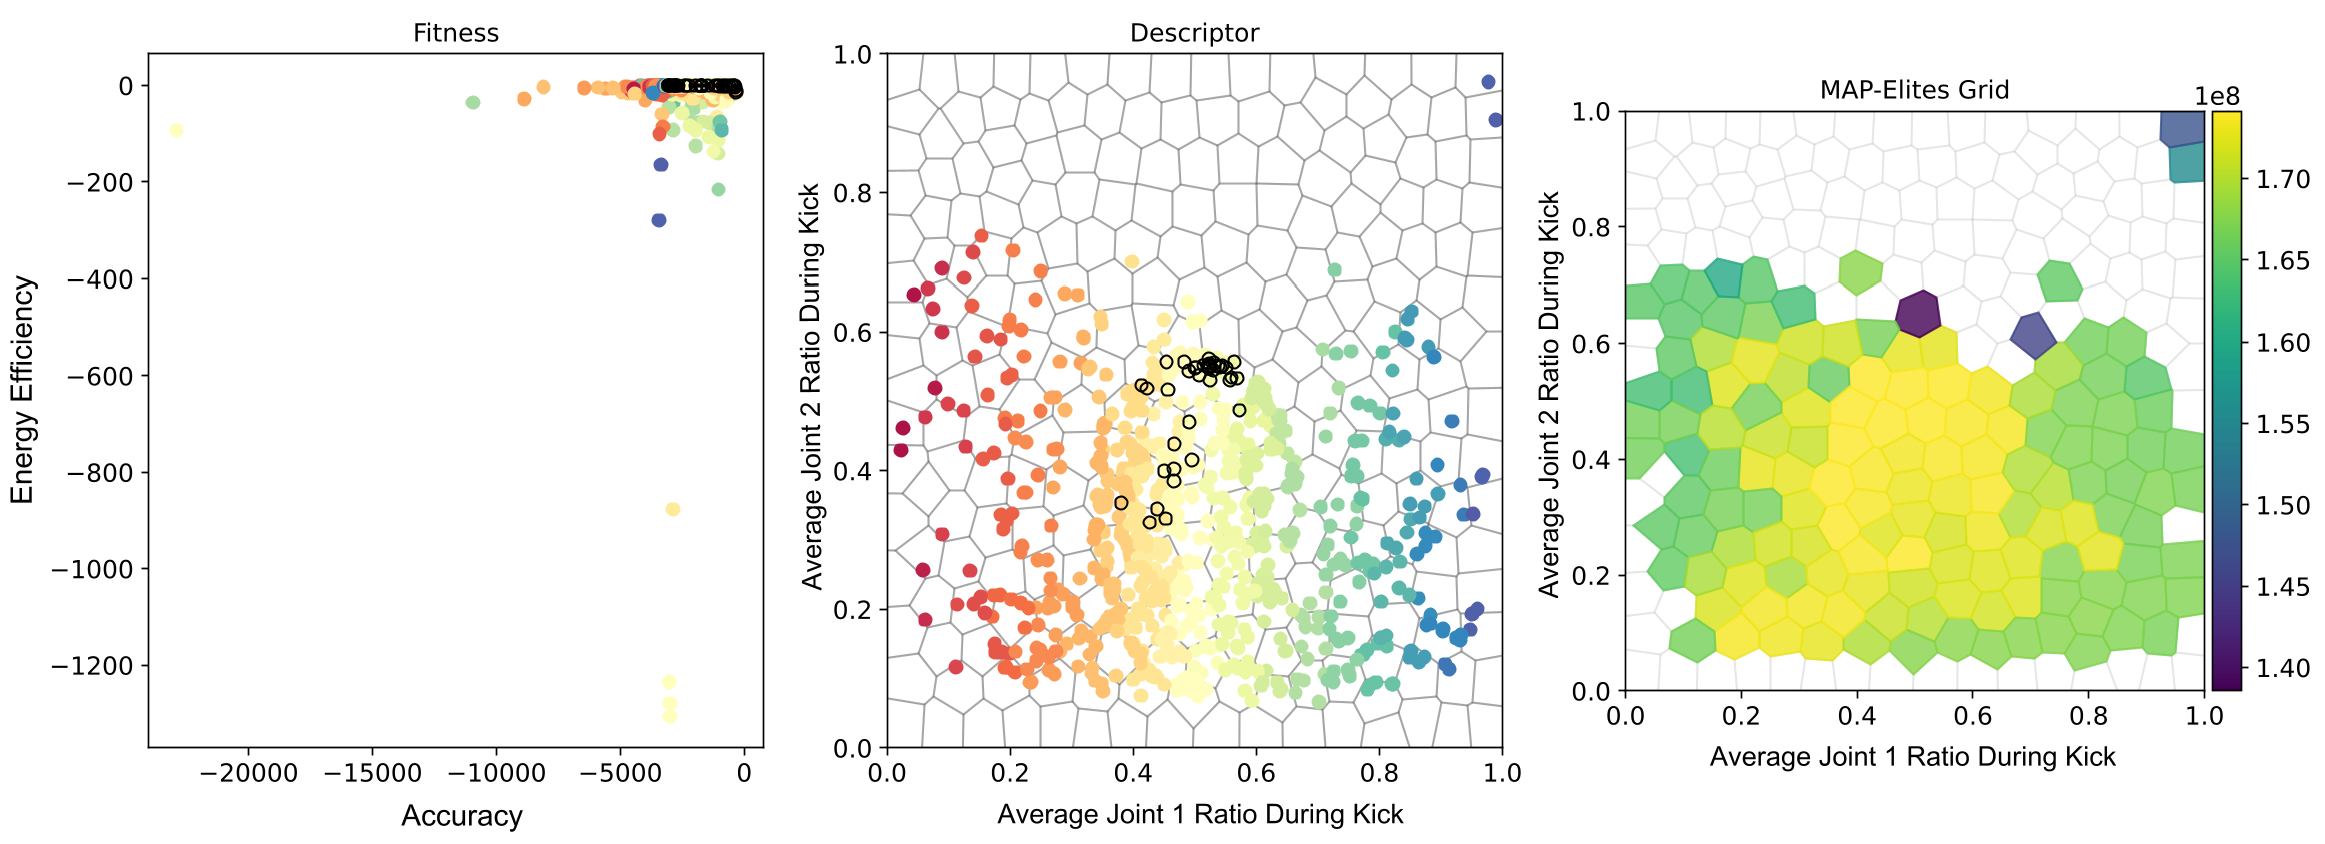
\includegraphics[width=0.96\textwidth]{Bilder/repertoire_walls_}
    \caption{Repertoire generated on the environment with walls: Global Pareto front (left); behavior space, with black circles marking the global Pareto front solutions (middle); MAP-Elites grid, with color intensity representing the hypervolume of the Pareto front in each cell (rigth).}
    \label{fig:episode_fitness_bs_baseline_walls}
\end{figure}

The best solution from this repertoire in terms of accuracy has a maximum Reward Distance of $-0.220$ and a minimum Reward Control of $-1.017$. The robot uses a quick, powerful kick of the ball to Wall 1 which then bounces to Wall 2 and finally reaches the goal. Figure \ref{fig:baseline_wall_best_sol_metrics} shows the rewards during this episode.
\begin{figure}[H]
    \centering
    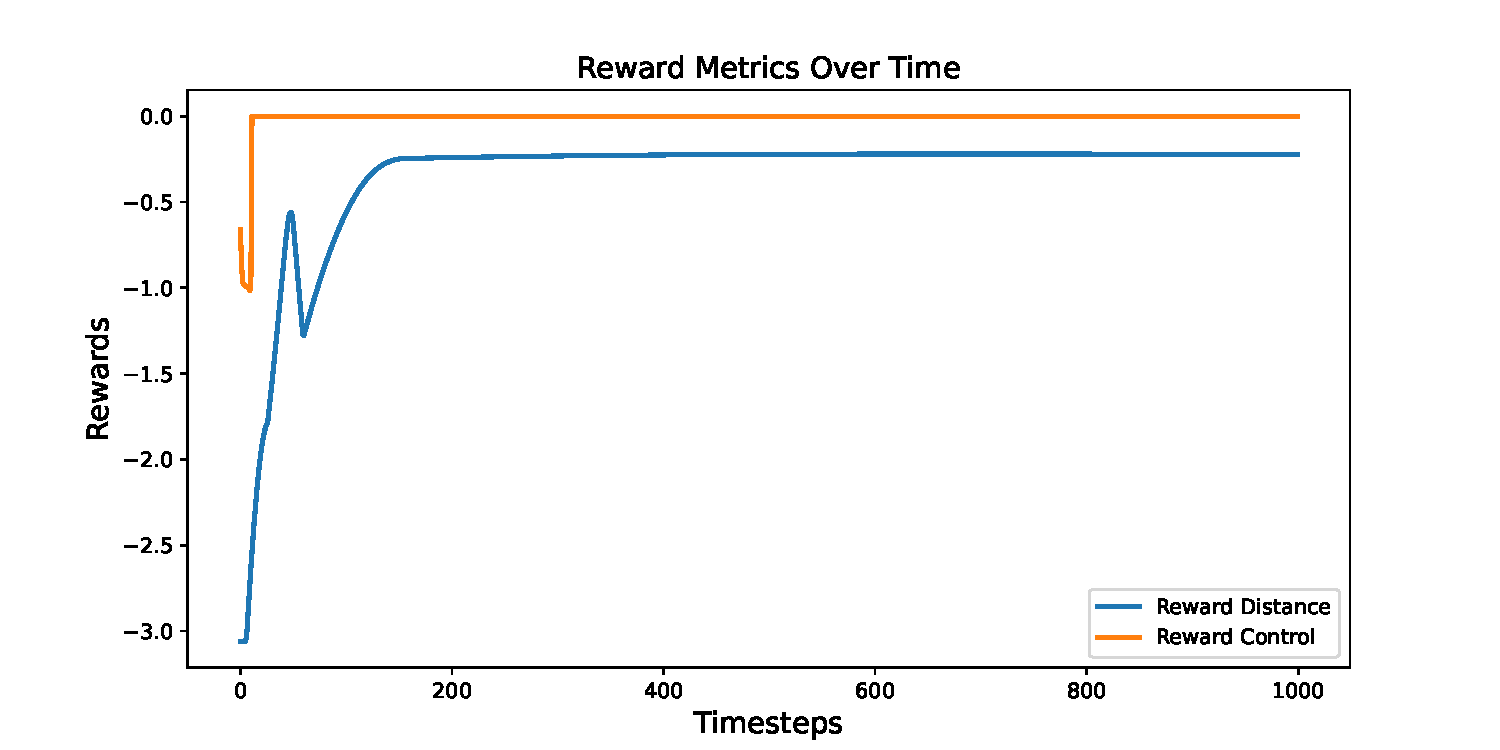
\includegraphics[width=0.9\textwidth]{Bilder/reward_metrics_wall}
    \caption{Rewards over time of the best solution found for the baseline environment with walls, where each line represents an individual reward at a time $t$.}
    \label{fig:baseline_wall_best_sol_metrics}
\end{figure}

\subsection{QD Algorithms Robustness} 
\subsubsection{Friction Coefficient Change}
The robot trained on the environment without walls is tested on environments with different friction values. Figure \ref{fig:accuracy_fvf} shows that the highest performance is achieved when the friction coefficient is 0.5, as this is the same used for training. A similar performance is achieved on the environment with a friction value of 0.4. However, on average, the robot’s performance in low-friction environments is comparable to that in high-friction environments. This is due to the way the fitness is calculated as described in Section \ref{metrics}: it is the cumulative sum of the rewards for accuracy, which is always negative (Equation \ref{eq:f1}). Therefore, this fitness is not necessarily an indicator that the robot hit or missed the goal, but rather of how far is the ball from the goal with respect to time. An alternative approach is discussed in Section \ref{limitations}.

The dots in the second part of the plot represent the performance (scaled) of the 50 tested solutions. For lower friction levels, the solutions performance are sparser compared with higher friction coefficients. Appendix \ref{appendix:gp_pred} shows the tested solutions and the GP predictions in the descriptor space for each friction value.

\begin{figure}[H]
    \centering
    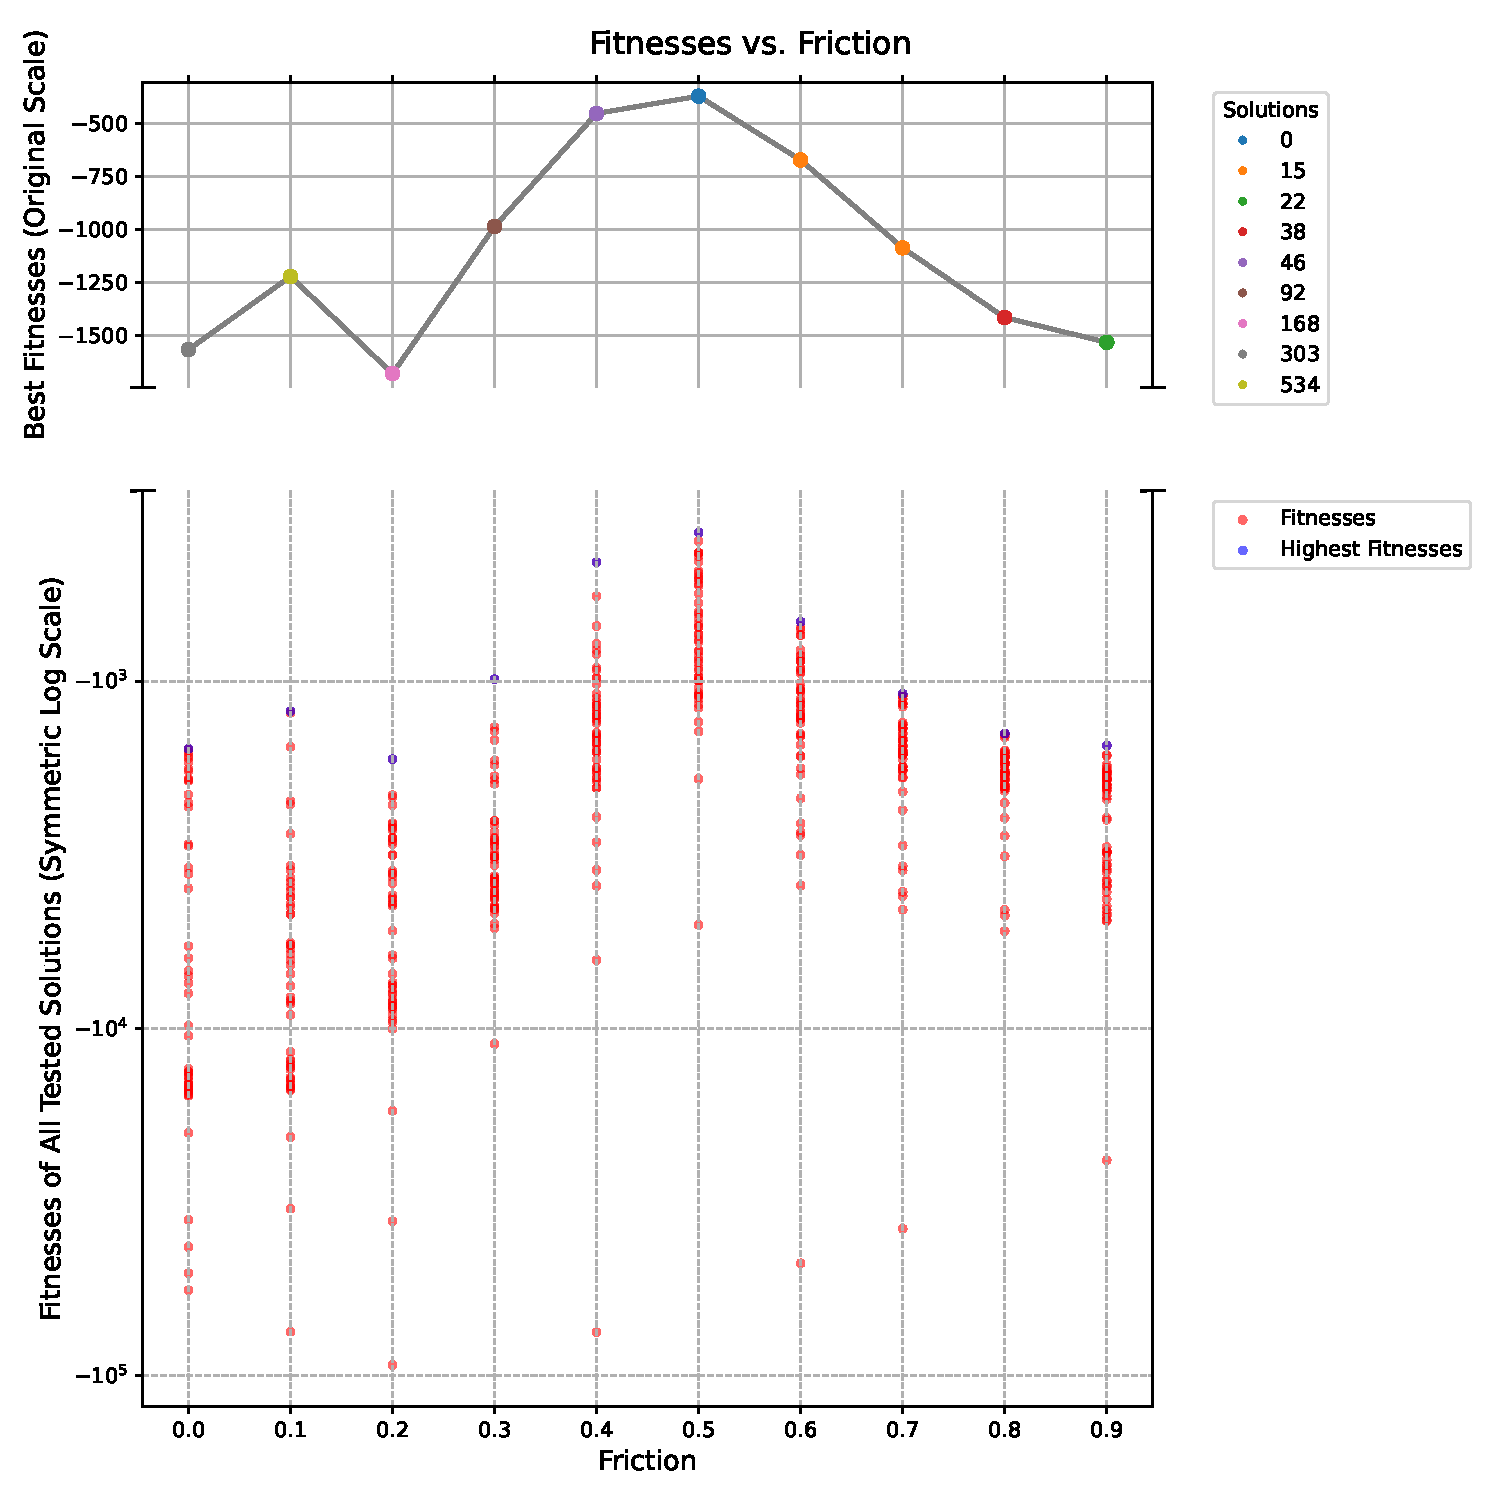
\includegraphics[width=0.9\textwidth]{Bilder/all_fvf}
    \caption{Accuracy fitnesses of the best solutions found for different friction levels, with dot colors indicating the corresponding solution index (upper plot). The lower plot shows the scaled fitnesses of all 50 tested solutions across the different friction environments.}
    \label{fig:accuracy_fvf}
\end{figure}
To better understand the trajectory of the ball, the minimum and final distance of the ball from the goal with respect to the friction values are shown in Figure \ref{fig:mfdf}. Here it is possible to see the reason for the poor performance of solution 168 found for the environment with friction coefficient of 0.2: the adaptation algorithm is not able to find a solution that kicks the ball in an accurate direction and with the necessary force to stop near the goal (for visualization of the minimum distance see Appendix \ref{appendix:vis}). 

In order to see how a solution found for a high-friction environment performs in other environments, solution 22 (found for the friction value of 0.9) is tested on all the environments and the closest and final distances are also shown below. It can be seen that it performs slightly better (in terms of minimum and final distances) for the environment with friction coefficient of 0.8. However, for the other environments it is worse due to the final distance: the ball ends up further due to the hard kick and low friction level. The minimum distance is also worse for the other environments (excluding the one with 0.2 friction coefficient), which indicates that the direction of the kick in solution 22 is not the most accurate. 

\begin{figure}[H]
    \centering
    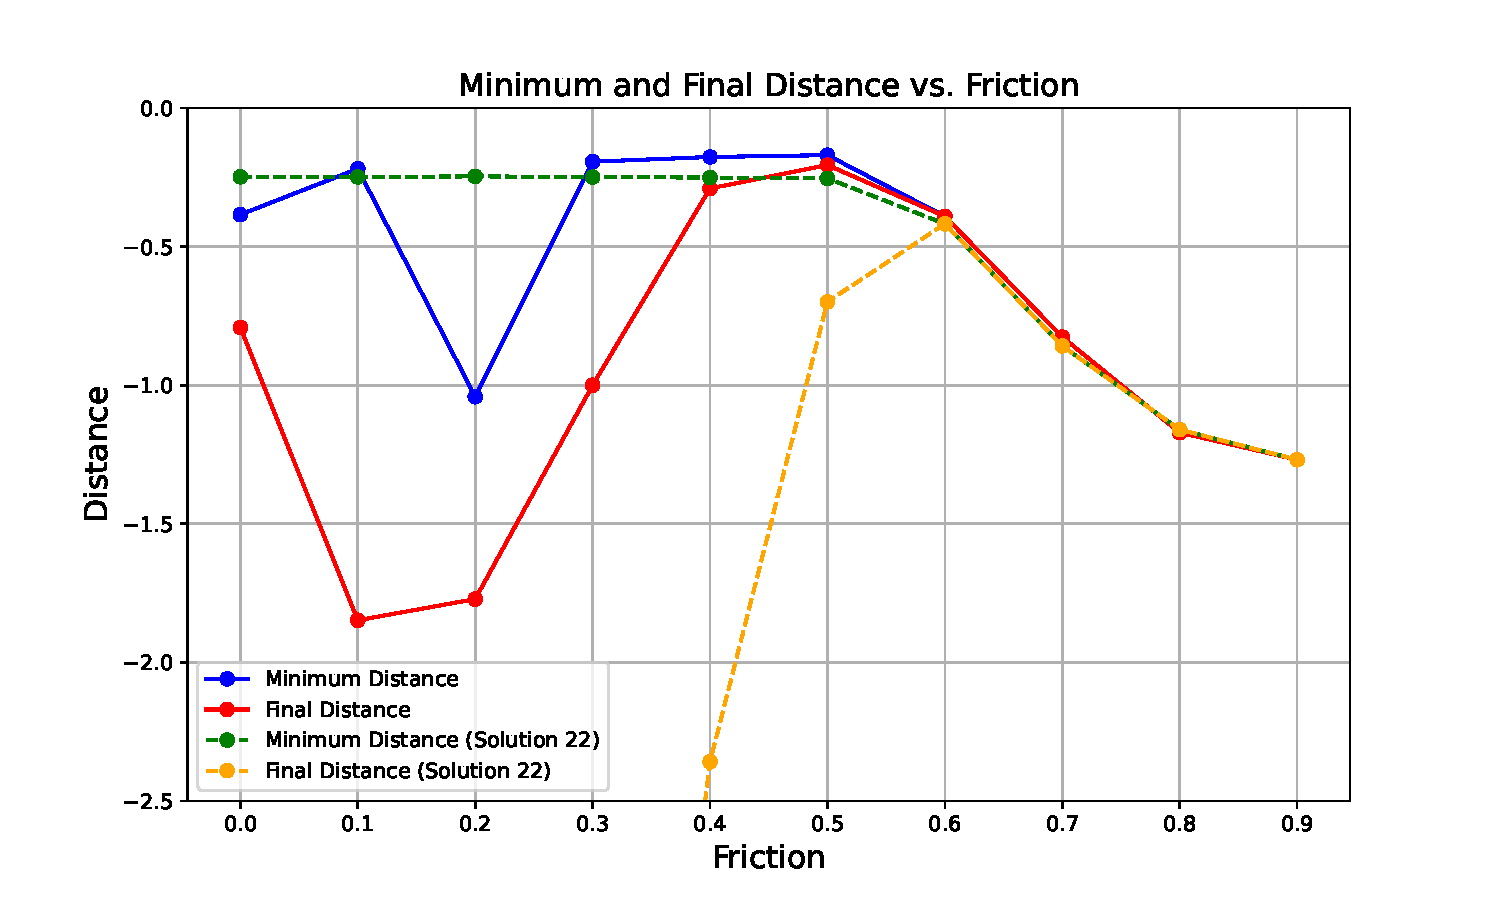
\includegraphics[width=0.9\textwidth]{Bilder/sol9_dvf}
    \caption{Minimum and final distances of the ball from the goal across different friction levels. The solid lines represent the best solutions found for each friction level tested, while the dashed lines correspond to the performance of Solution 22, specifically found to be the best performing in the environment with a friction coefficient of 0.9.}
    \label{fig:mfdf}
\end{figure}
Nevertheless, the training and adaptation process are made with respect to the fitness, where the minimum and final distances are not explicitly considered. Therefore, in Figure \ref{fig:mfdff} the actual fitnesses are shown, where the blue line represents the performance of the best solution from the simulation tested in different environments, the green line is the performance of each of the solutions found during the adaptation process, and the red one is the performance of the solution 22 in the different environments. The fitnesses from the found solutions clearly outperform the other two categories in every environment. 
\begin{figure}[H]
    \centering
    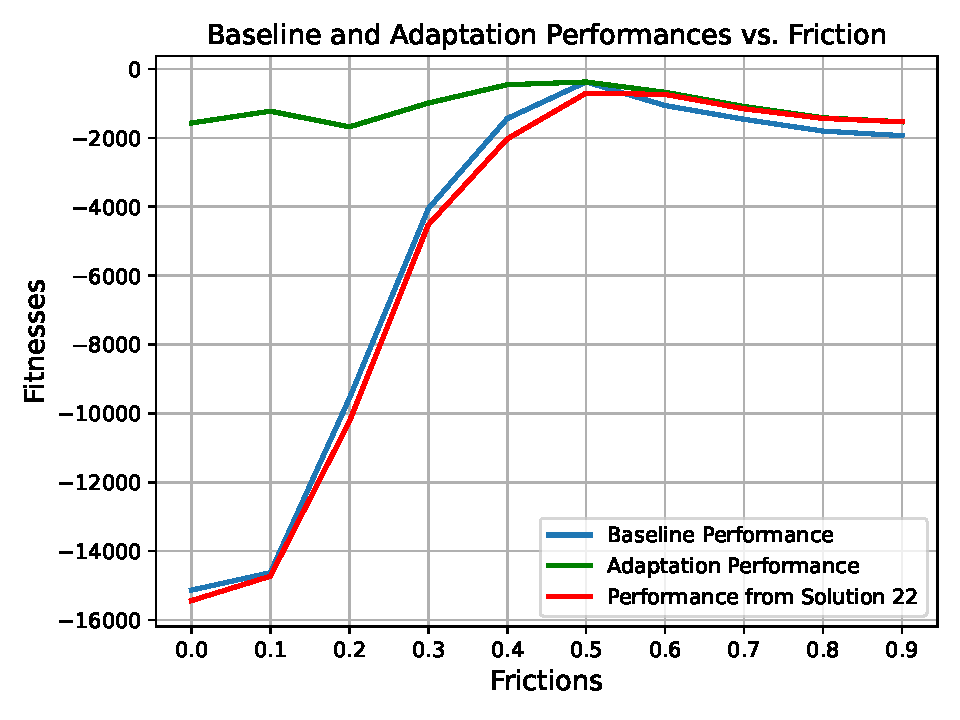
\includegraphics[width=0.8\textwidth]{Bilder/performances_friction}
    \caption{Fitness of the best solution from simulation tested on different friction values (blue), the fitness of the best solutions found for each friction level during adaptation (green), and fitness of the solution 22 tested on the different environments (red).}
    \label{fig:mfdff}
\end{figure}
The best performance evolution in each environment with respect to environment steps is shown in Figure \ref{fig:perf_ev}. It is important to notice that, on average, the algorithm needs $3.1 \times 10^{4}$ environment steps (which is equivalent to 31 tests in reality) to find the optimal solution for the unknown environments, being $4.9\times 10^{4}$ the longest it took for the environments with friction coefficient of 0.3 (see Figure \ref{fig:density}). 
\begin{figure}[H]
    \centering
    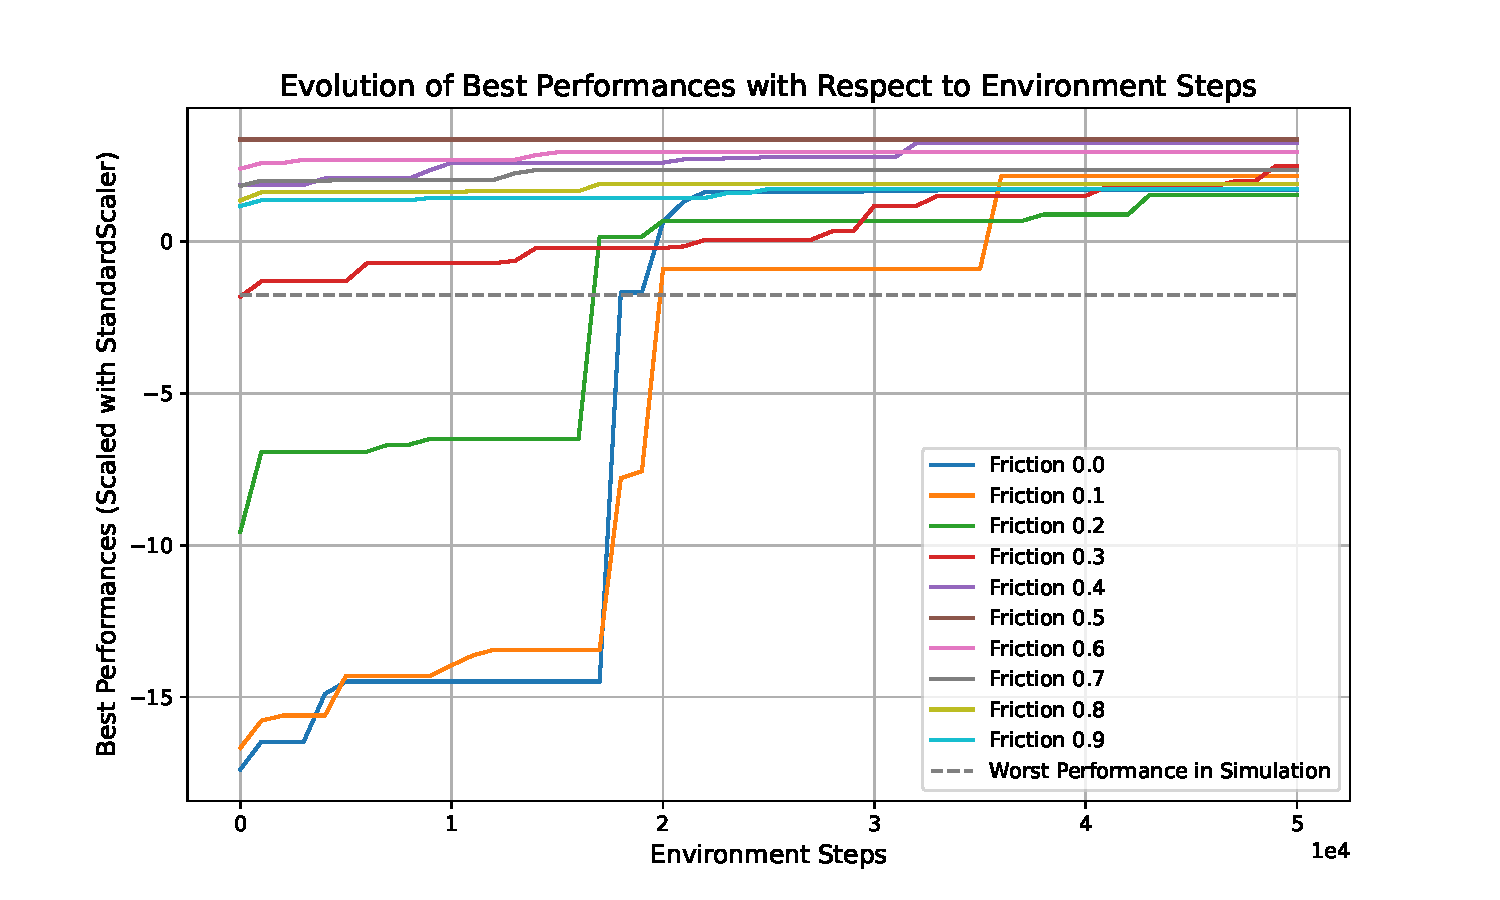
\includegraphics[width=1.0\textwidth]{Bilder/best_evolution}
    \caption{Best performance evolution during adaptation for environments with different friction coefficients.}
    \label{fig:perf_ev}
\end{figure}
Considering the range between worst and best performances from the simulation (dashed and brown lines respectively), the adaptation process achieves a relatively high performance for friction values of $0.5\pm0.1$ as can be seen in Figure \ref{fig:density}. 

If the robot is required to kick the ball and reach the target without considering the final distance, then the low-friction environments would have a higher performance because the solutions would not be bounded by a maximum force that could be applied (i.e. it could be a strong kick as long as it goes close to the goal), resulting in a higher variety of suitable solutions. 

\begin{figure}[h]
    \centering
   % 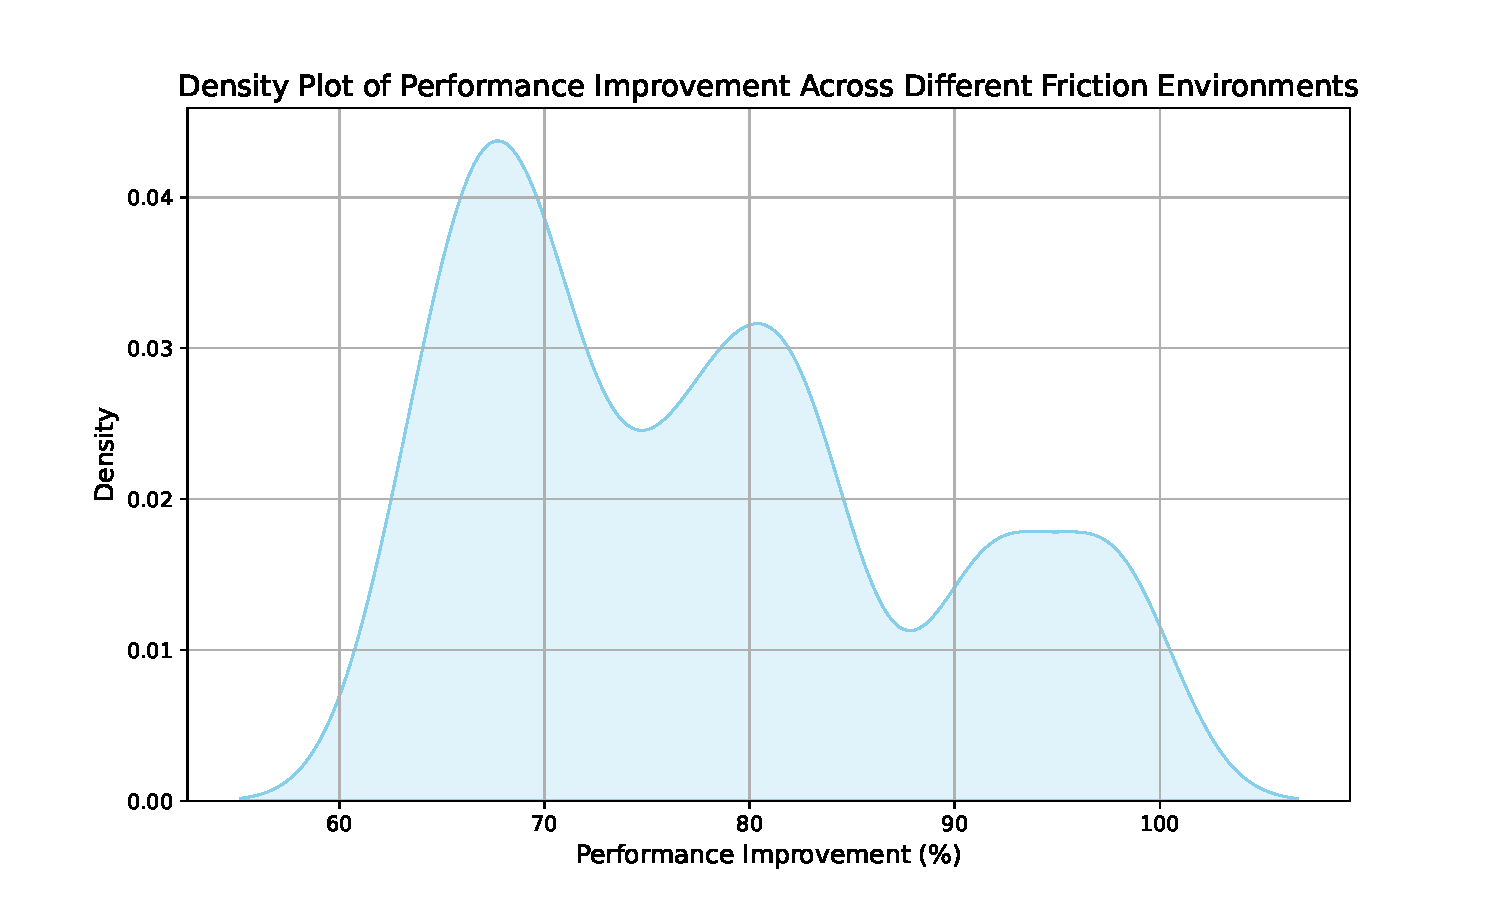
\includegraphics[width=1.0\textwidth]{Bilder/performance_improvement_density}
    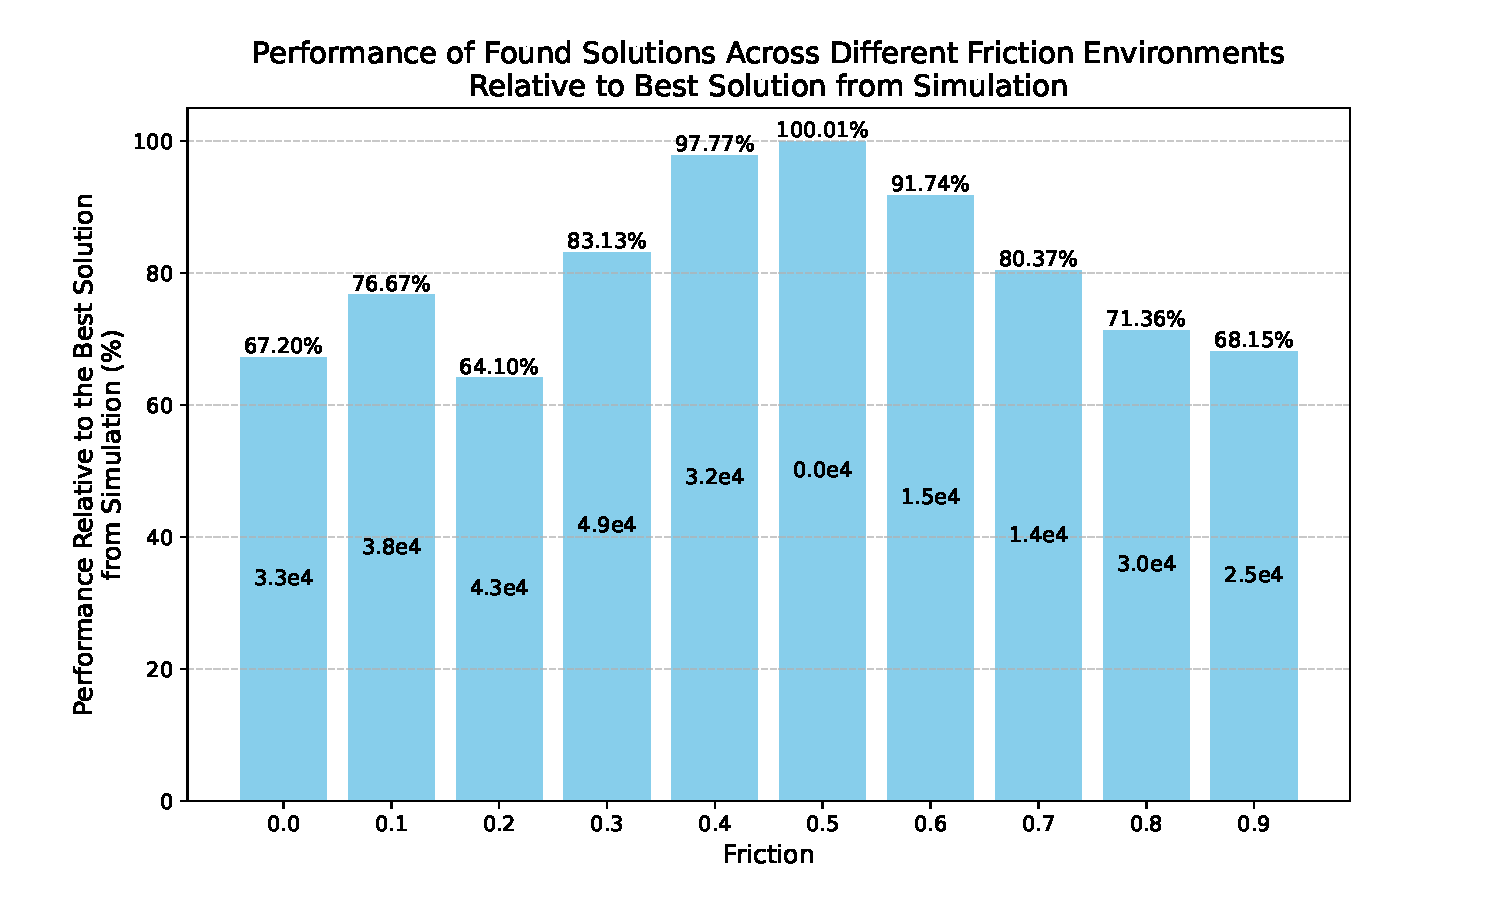
\includegraphics[width=1.0\textwidth]{Bilder/performance_percentage_friction_it}
    \caption{Performance of the best solution found in environments with different friction values with respect to the best performing solution from the simulation. The values inside the bars are the number of environment steps needed to find the respective solution.}
    \label{fig:density}
\end{figure}

The adaptation of the robot trained with MOME-PGX proves to be successful when the friction level varies by $\pm 0.1$ from the friction coefficient of the simulation and adapting from a repertoire of already learned behaviors is more efficient than learning an entire repertoire from scratch: $3.1 \times 10^{4}$ vs. $5000 \times 10^{4}$  environment steps. This means that adapting is approximately $1600$ times faster (considering all the tested friction values) at the expense of losing $\leq 10\%$ of the performance, which is an acceptable trade-off for situations in which the quick adaptation is vital. 


\subsubsection{Obstacle Height}
The baseline environment without walls is tested on environments with a barrier in front of the ball, with varying heights. The performance of the solutions found during the adaptation process can be seen in Figure \ref{fig:adapt_obs}. 

In the performance evolution plot (Figure \ref{fig:perf_ev_obs}) and in Figure \ref{fig:perf_imp_obs}, it is possible to see that for heights below $0.06\ \text{m}$, the average environment steps necessary to find the best solution are $1.4\times 10^{4}$. However, for $0.06\ \text{m}$ and $0.07\ \text{m}$, the algorithm required more steps. 

The performance improvement after adaptation with respect to the range between minimum and maximum performance from simulation (Figure \ref{fig:perf_imp_obs}) indicates that a relatively high performance is achieved with an obstacle of height up to $0.02\ \text{m}$.

The adaptation process is approximately 2300 times faster (considering all the tested heights) than learning the entire repertoire, since it takes an average of $2.1 \times 10^{4}$ environment steps to find the best solution. 

\begin{figure}[H]
    \centering
    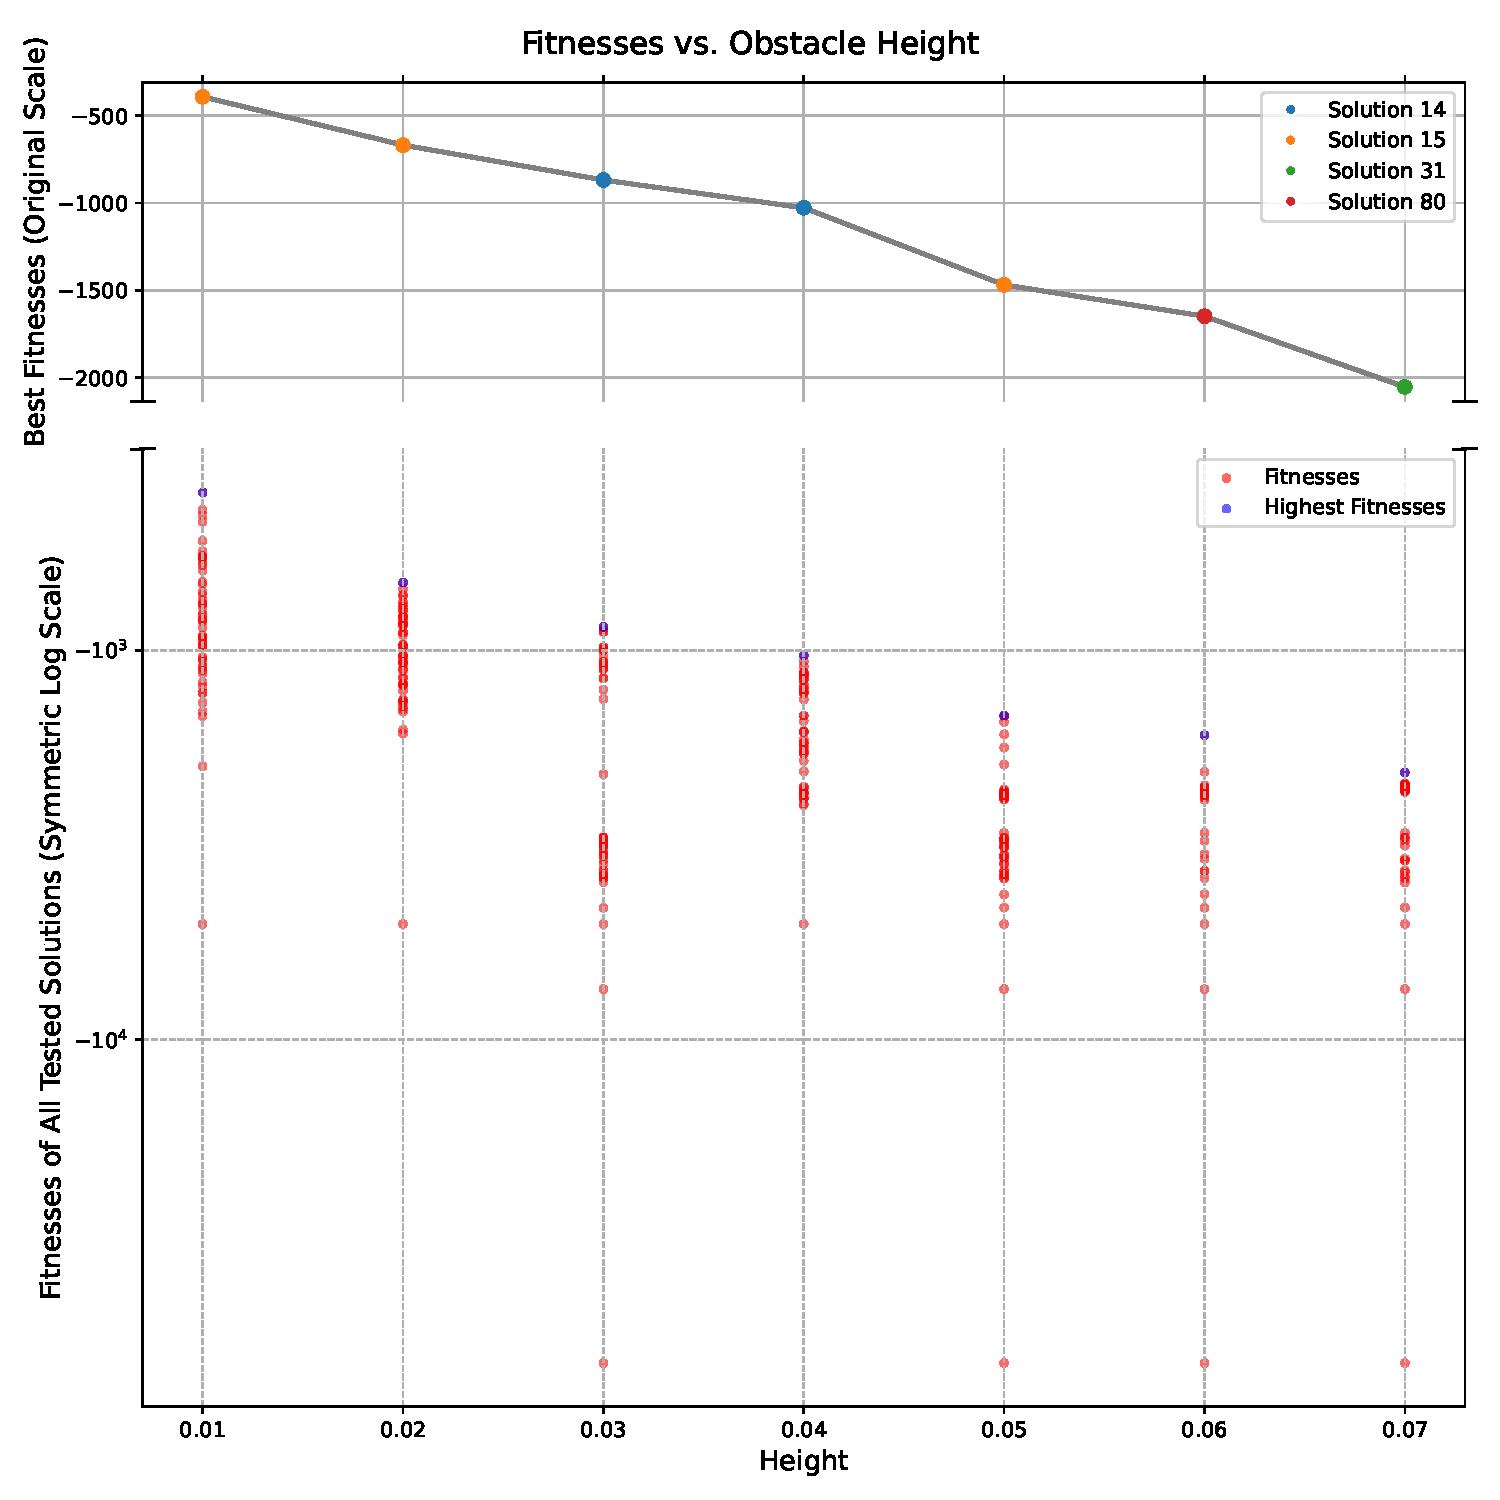
\includegraphics[width=1.0\textwidth]{Bilder/all_fvh}
    \caption{Accuracy fitnesses of the best solutions found for different obstacle heights, with the color of the dots representing the solution index (upper plot); scaled fitnesses of all 50 tested solutions for the different obstacle heights (lower part).}
    \label{fig:adapt_obs}
\end{figure}


\begin{figure}[h]
    \centering
    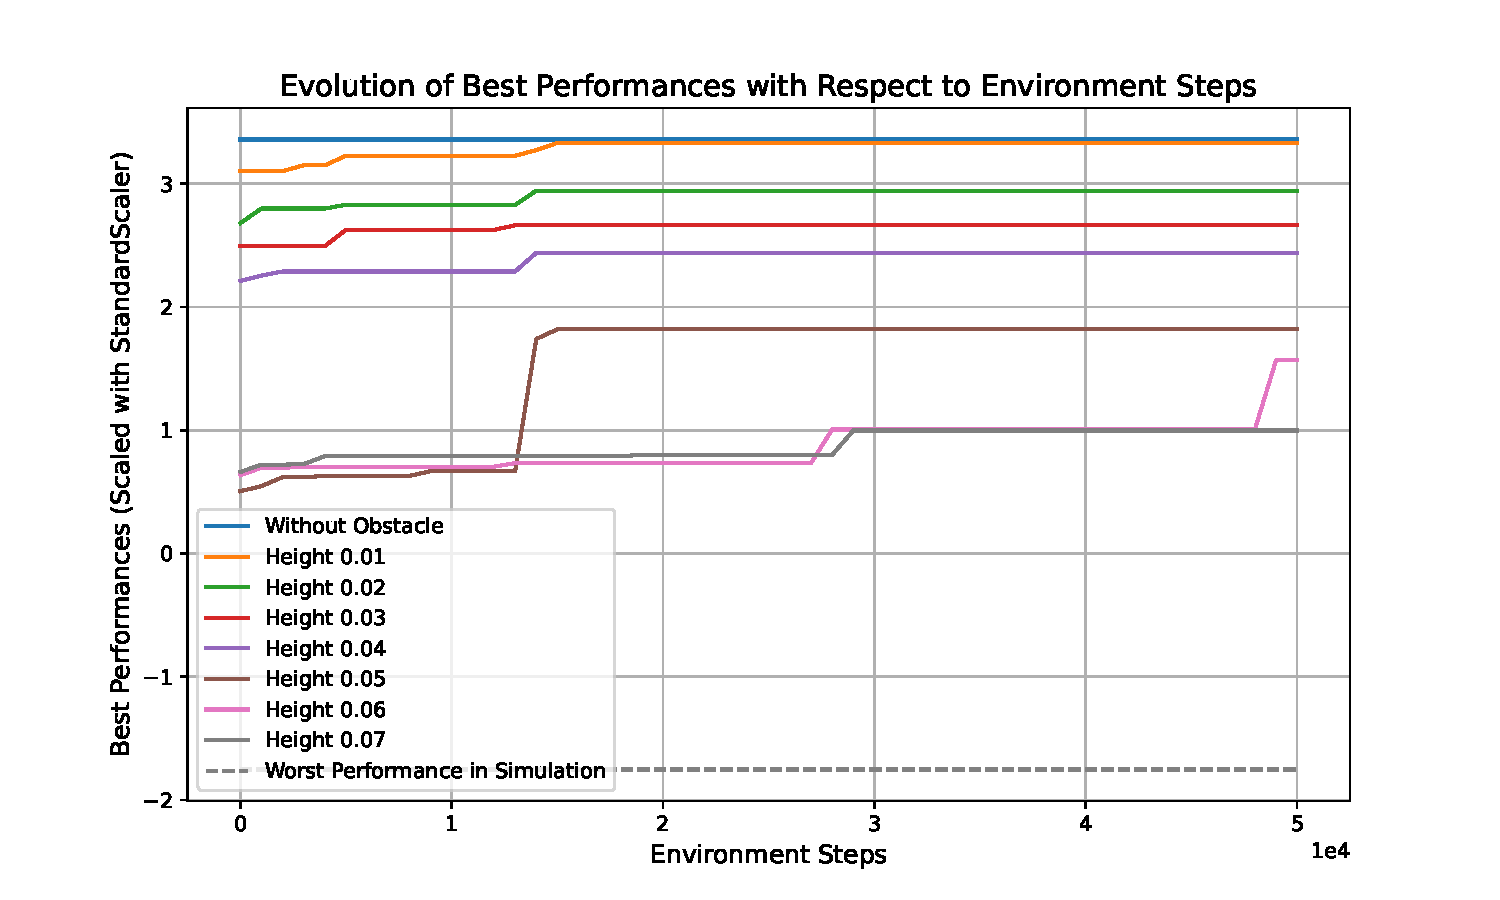
\includegraphics[width=0.95\textwidth]{Bilder/best_evolution_obstacle}
    \caption{Best performance evolution during adaptation for environments with obstacles of different heights.}
    \label{fig:perf_ev_obs}
\end{figure}

\begin{figure}[H]
    \centering
    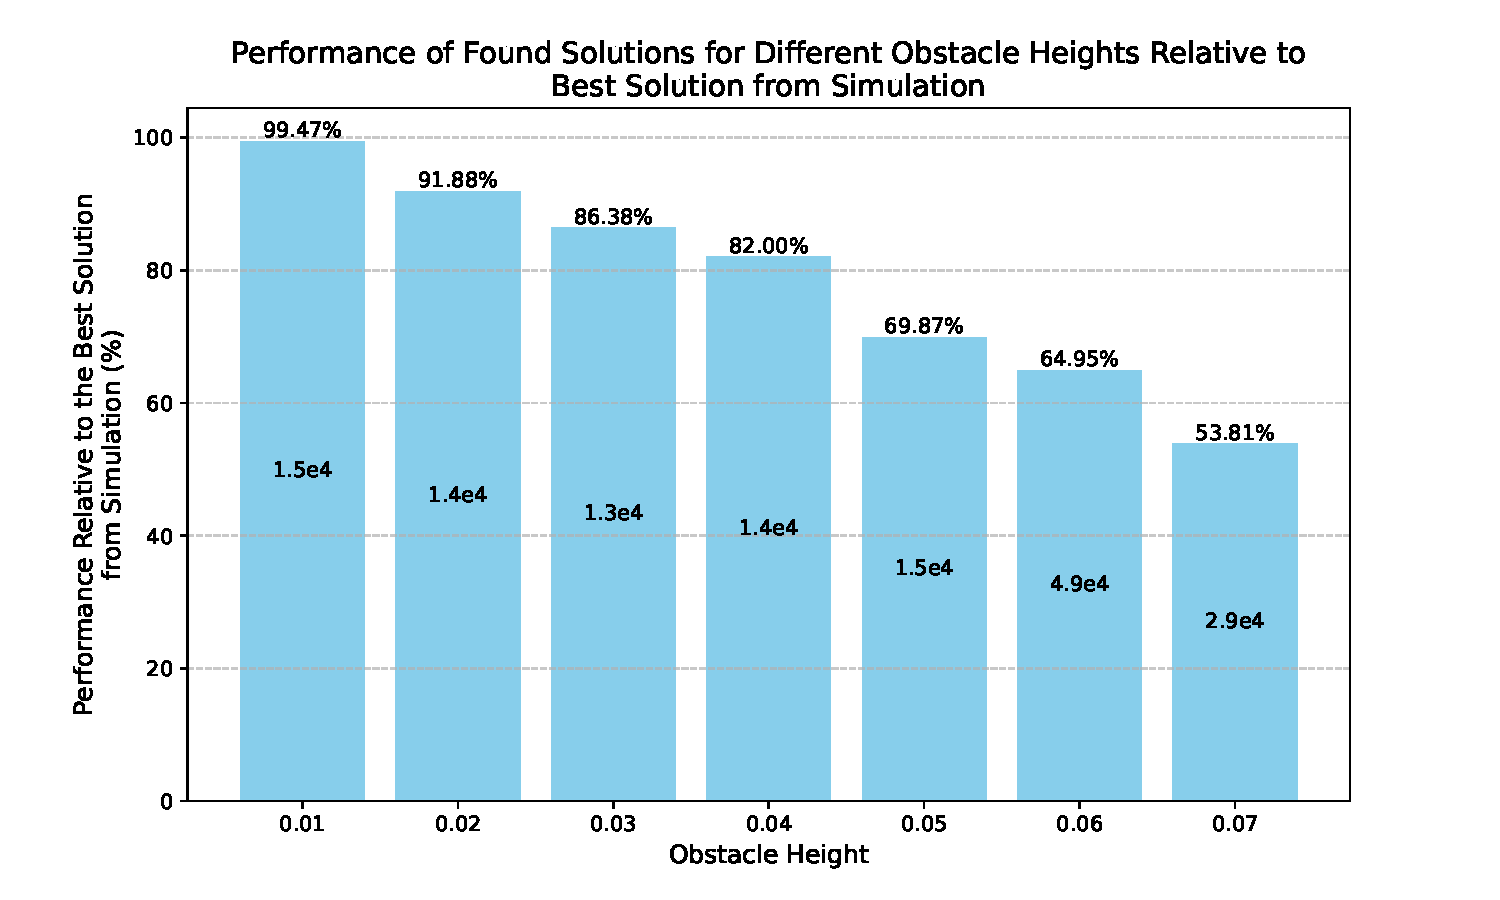
\includegraphics[width=0.95\textwidth]{Bilder/performance_percentage_height_it}
    \caption{Performance of the best solution found in environments with obstacles of different heights with respect to the best performing solution from the simulation. The values inside the bars are the number of environment steps needed to find the respective solution.}
    \label{fig:perf_imp_obs}
\end{figure}

%\begin{figure}[H]
%    \centering
%    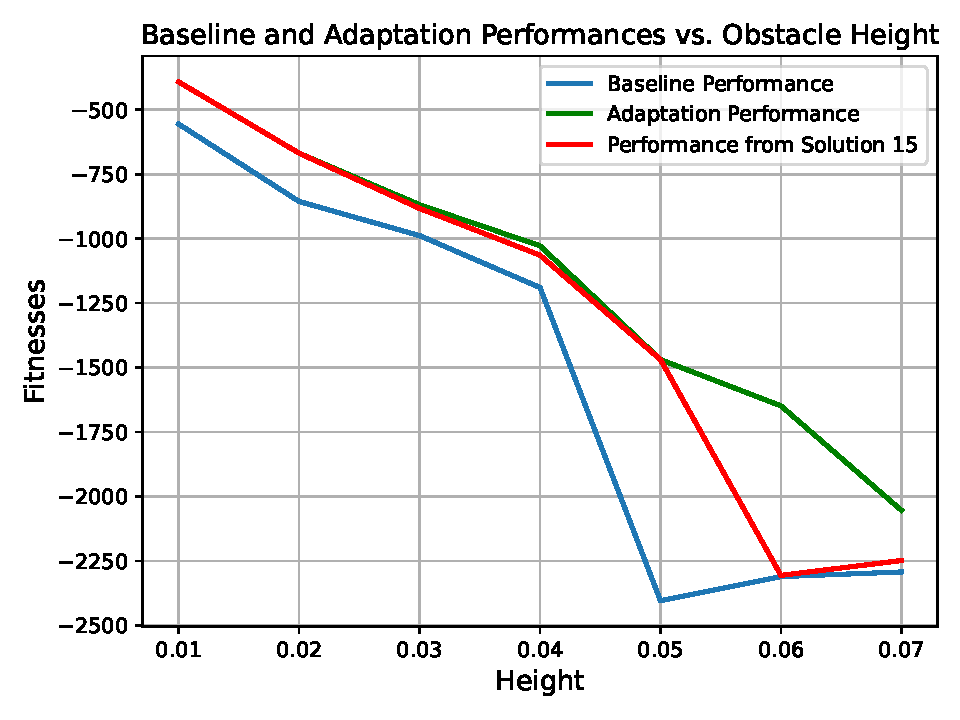
\includegraphics[width=0.8\textwidth]{Bilder/performances_height}
%    \caption{Performance}
%    \label{fig:perf_obs}
%\end{figure}

\subsubsection{Walls}
When the robot that is trained with two walls is tested only with Wall 1, it takes the algorithm $0.3 \times 10^{4}$ environment steps (3 tests in reality) to reach the highest performing solution, which uses the available wall to reach the goal. Meanwhile, in the environment with Wall 2, it takes $1.0\times 10^{4}$ environment steps (10 tests in reality) and the solution does not use the available wall. The solutions reach $99.87\%$ and $99.48\%$ of the best solution from simulation respectively.


\begin{figure}[H]
    \centering
    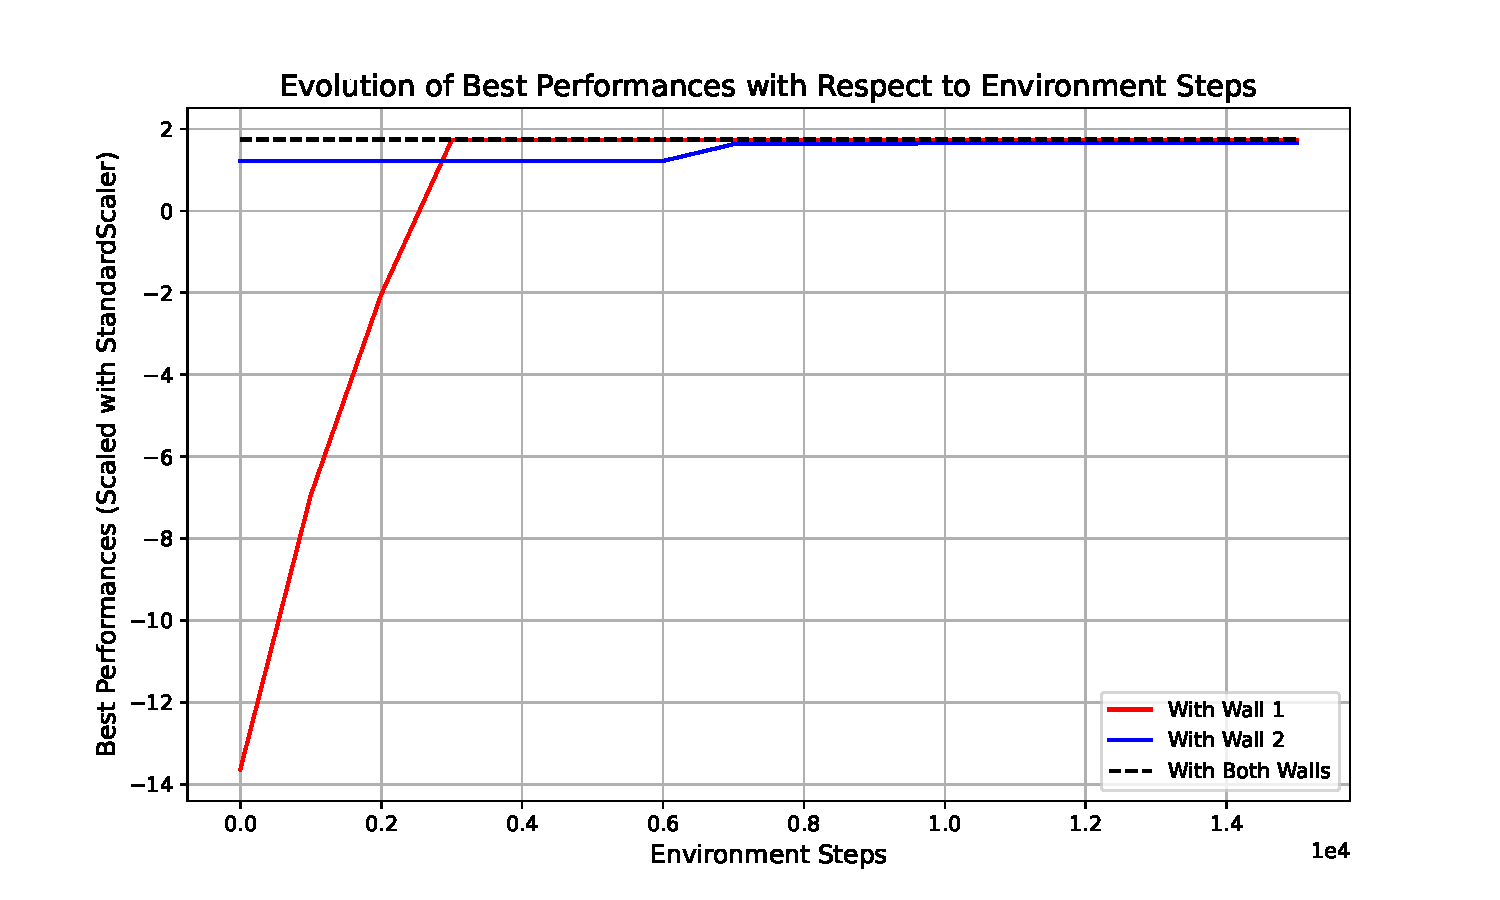
\includegraphics[width=1.0\textwidth]{Bilder/best_evolution_walls}
    \caption{Best performance evolution during adaptation for environments with different ways of reaching the goal (walls).}
    \label{fig:best_ev_walls}
\end{figure}
It is possible to visualize the adaptation process in Figure \ref{fig:adapt_walls}, where each dot is a solution tested in the unknown environment and their color represent their measured performance scaled with StandardScaler. The contour map shows the Gaussian Process predicted offset after evaluating the last solution. It is interesting to see that for the environment with Wall 1, there are two groups of suitable solutions: using the available wall or kicking the ball directly to the goal. However, in the environment with Wall 2, there are no solutions found that use the wall, but only kicking the ball directly to the goal. This can be due to the placement of the walls which is not completely symmetric, where Wall 1 is closer to the goal.

\begin{figure}[H]
    \begin{minipage}[t]{0.95\linewidth}
        \centering
        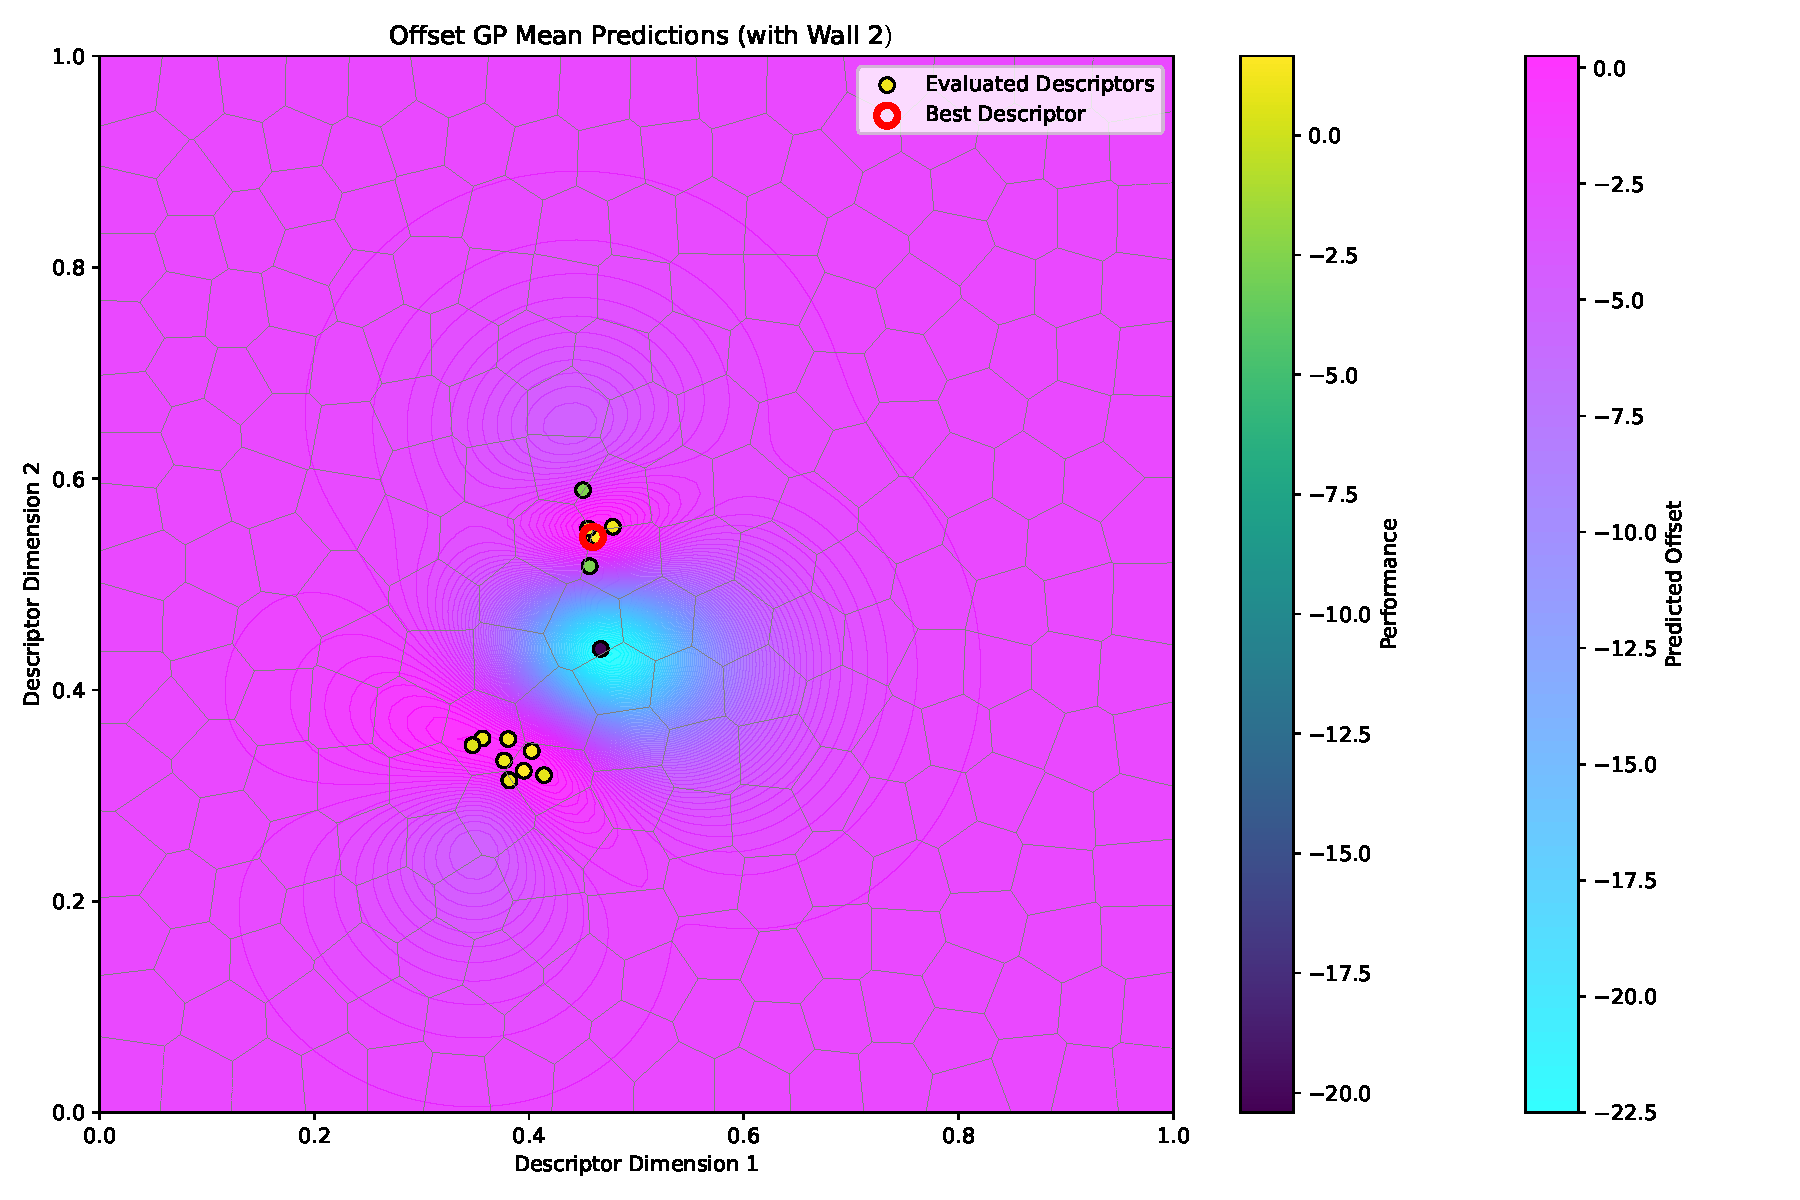
\includegraphics[width=\linewidth]{Bilder/omp_with_voronoi_wall2}
    \end{minipage} 
    \begin{minipage}[t]{0.95\linewidth}
        \centering
        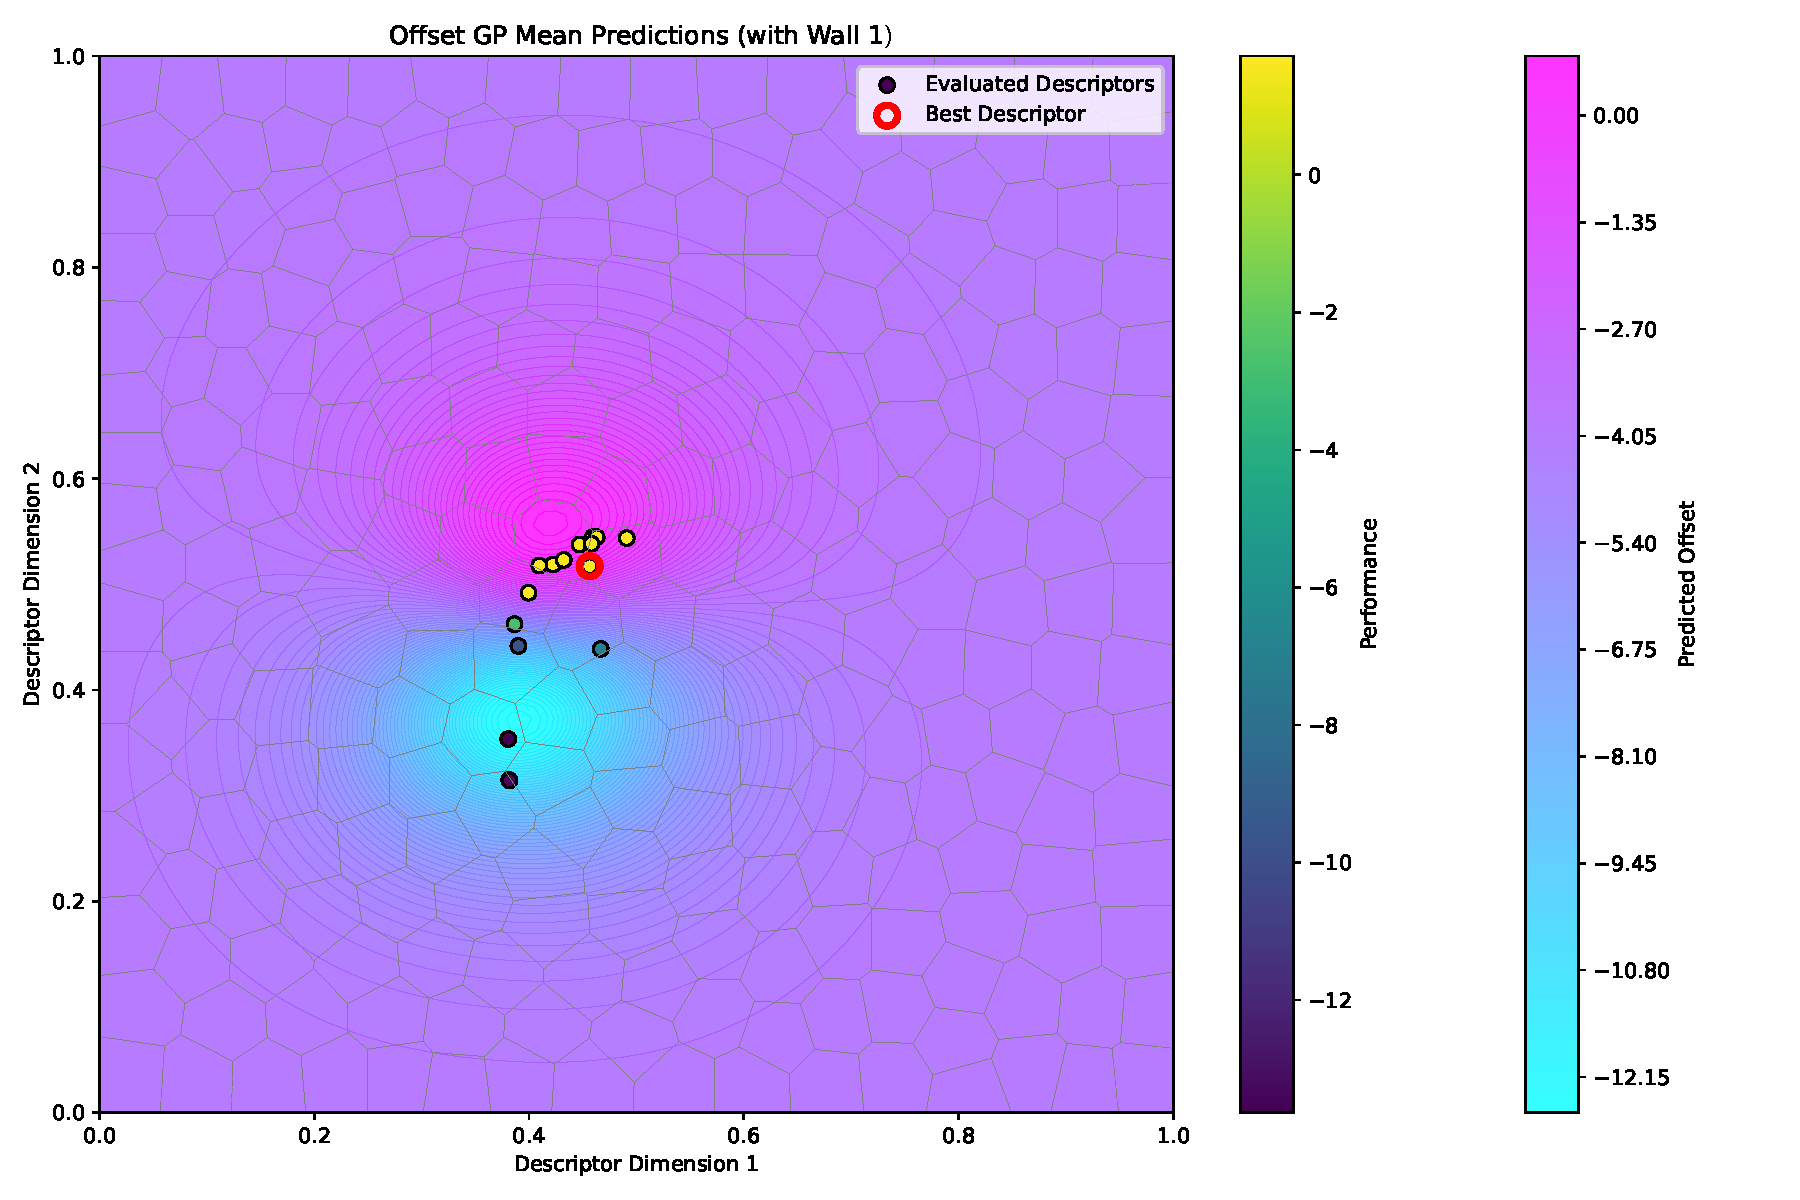
\includegraphics[width=\linewidth]{Bilder/omp_with_voronoi_wall1}
    \end{minipage} 
    \caption{Visualization of the adaptation process, where each dot is a tested solution, their color is their real performance, and the contour map represents the GP offset prediction. The best solution is marked by the red ring.}
    \label{fig:adapt_walls}
\end{figure}



\subsection{Exploration Criterion}
After adding the exploration criterion to the $x$ axis of the MAP-Elites grid, this is the generated repertoire:
\begin{figure}[H]
    \centering
    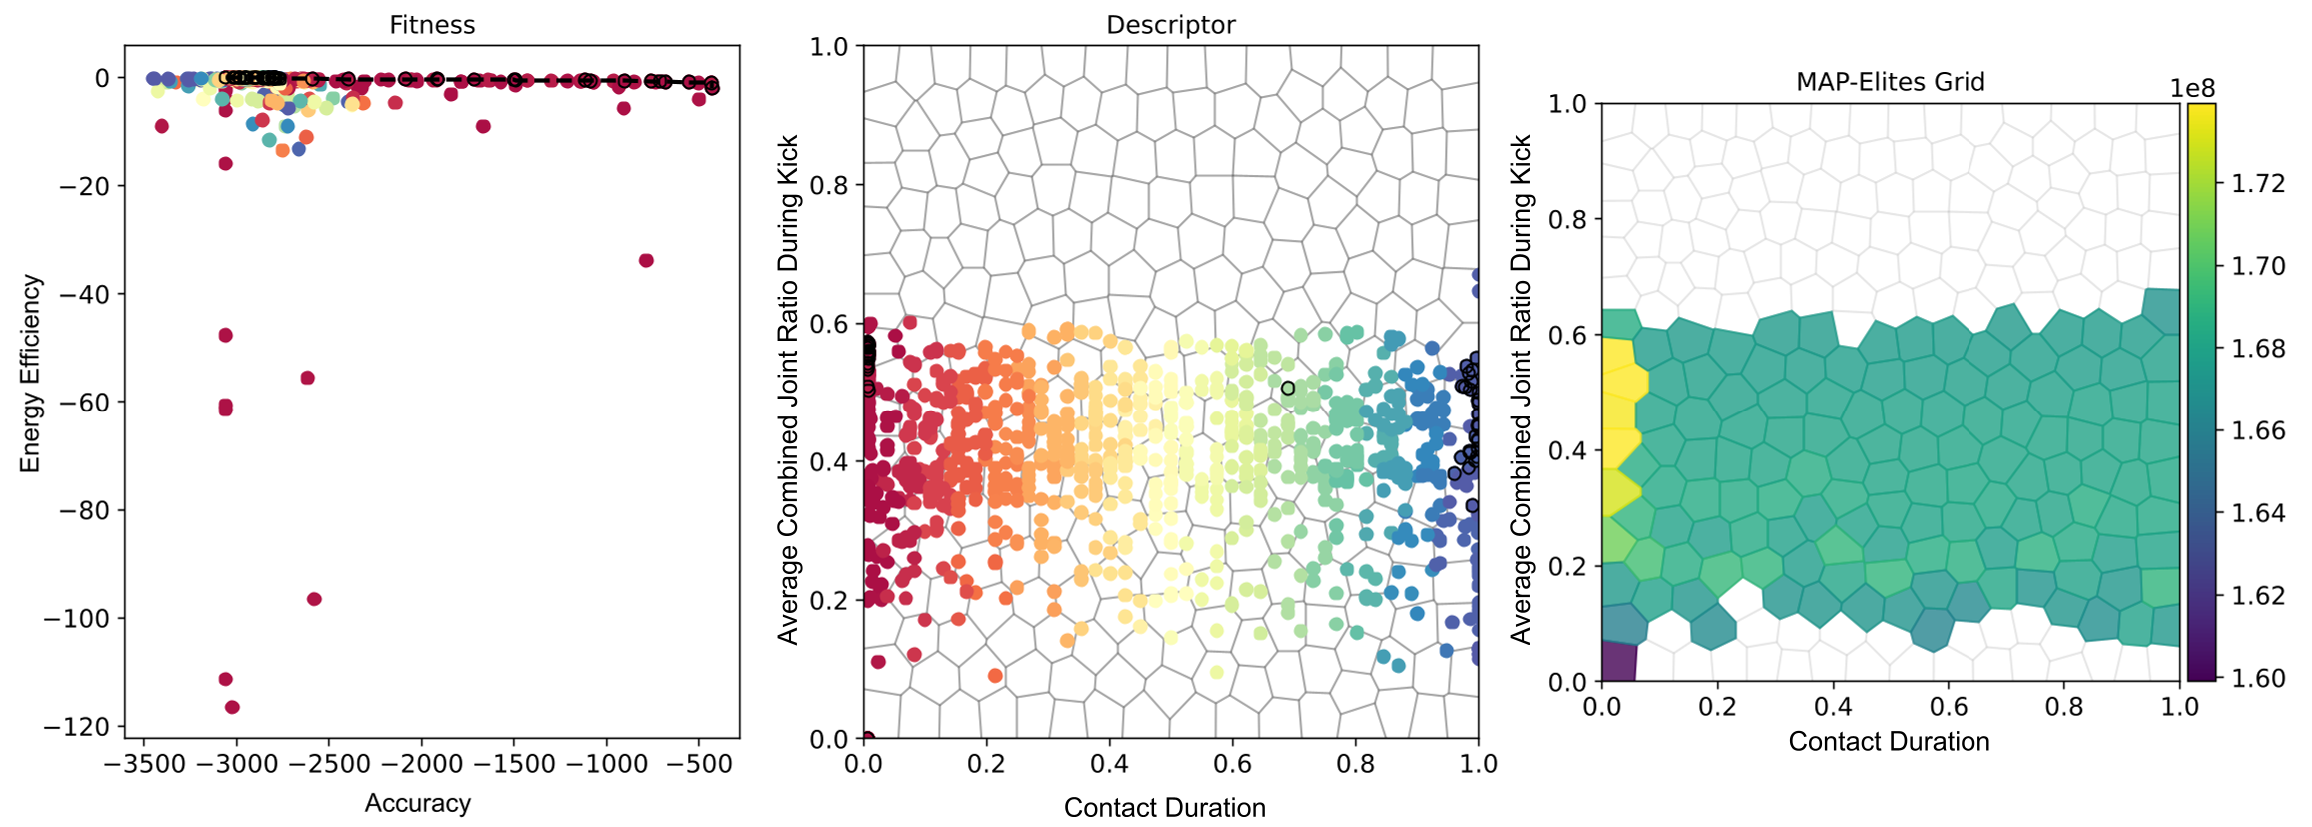
\includegraphics[width=1.0\textwidth]{Bilder/repertoire_final_exp_}
    \caption{Repertoire generated with the exploration criterion: Global Pareto front (left); behavior space, with black circles marking the global Pareto front solutions (middle); MAP-Elites grid, with color intensity representing the hypervolume of the Pareto front in each cell (rigth).}
    \label{fig:repertoire_exp}
\end{figure}

The red solutions correspond to short contact kicks and the blue ones are the long contact ones. The solutions that constitute the global Pareto front are on the extremes of the $x$ axis, meaning that they consist on either short kicks or notably long ones. This is because the short kicks are more effective to kick the ball near the goal, while the long kicks use less energy, but are less accurate. In Figure \ref{fig:scores_ev_exp}, the MOQD score and coverage increase at a higher rate than the training without the exploration criterion (Figure \ref{fig:scores_evol_baseline}), but they reach lower values: MOQD score of $2.2\times 10^{10}$ and coverage of $51.95\%$. 

The generation of the repertoire without the exploration criterion reaches a MOQD score of $2.0\times 10^{10}$ after approximately $2.6\times 10^{7}$ environment steps, while the one with the exploration criterion reaches $2.0\times 10^{10}$ after $1.0\times 10^{7}$ environment steps, which shows that, up to a score of $2.0\times 10^{10}$, the exploration criterion is 2.6 times faster, but then the values increase slower up to $2.2\times 10^{10}$, while the training with the exploration criterion keeps increasing up to $2.6\times 10^{10}$.

\begin{figure}[H]
    \centering
    \begin{minipage}{0.5\textwidth}
        \centering
        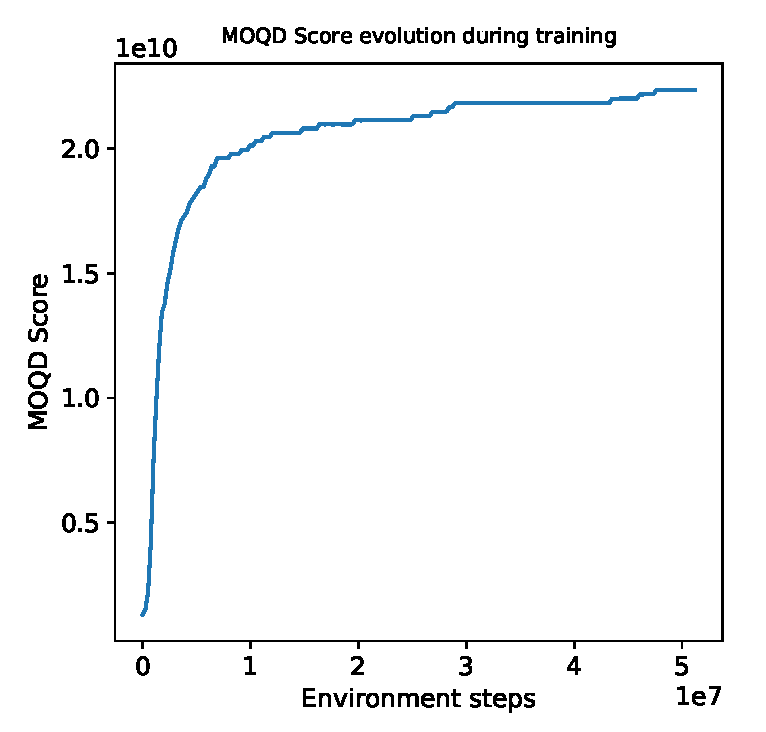
\includegraphics[width=\textwidth]{Bilder/scores_ev_exp1}
        \label{fig:image1}
    \end{minipage}\hfill
    \begin{minipage}{0.5\textwidth}
        \centering
        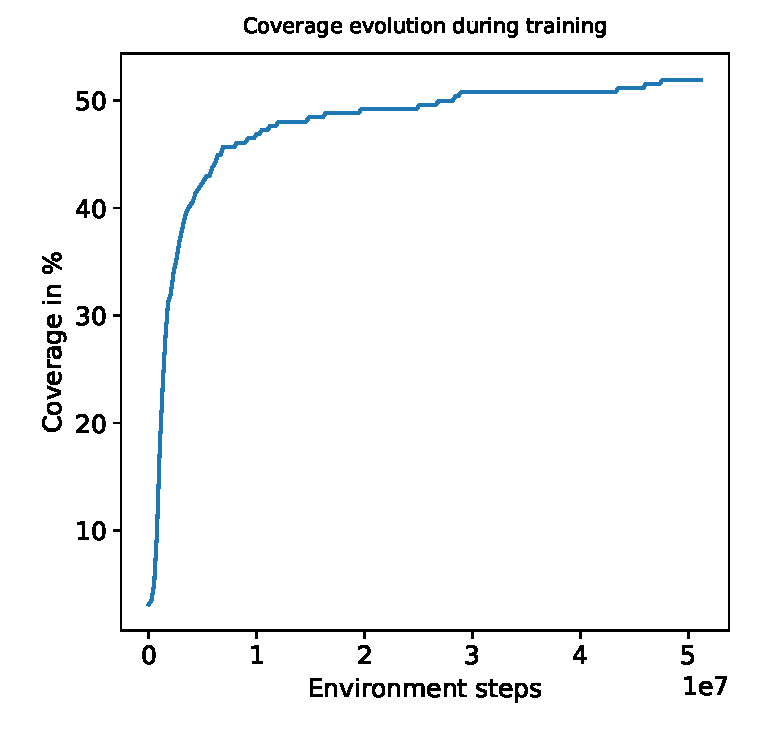
\includegraphics[width=\textwidth]{Bilder/scores_ev_exp2}
        \label{fig:image2}
    \end{minipage}
    \caption{Scores evolution during training with the exploration criterion.}
    \label{fig:scores_ev_exp}
\end{figure}



%%%%%%%%%%%%%%%%%%EVALUATION%%%%%%%%%%%%%%%%%%%%%%%%%%%%%%%%%%%%%%%%%%%
\subsection{Limitations} \label{limitations}
Even though the experiments are conducted in a simulated environment, the inaccuracies introduced make the results applicable to certain real environments. However, in this study, only one aspect (such as friction value or obstacle height) is purposefully adjusted at a time to explore its effect on the robot’s performance. In non-controlled environments, not only one factor can change, other parameters such as ground texture, inclination, and the presence of unexpected obstacles can be present simultaneously. That is why taking this study to a real-world environment would make the results even more generalizable.  

It is important to note that the obtained adaptation results for the friction coefficient, obstacle, and walls experiments apply to the chosen behavior descriptors, which were used due to their computation simplicity. However, it would be possible to choose better descriptors that characterize the kicking behavior in a better, more detailed way, such as including the kicking force, the initial velocity of the ball, or the angle of contact. These higher-dimensional descriptors would increase complexity but could also enhance the diversity of the repertoire, making it more versatile in environments with larger simulation-reality offsets. 

The specific results are related to the particular robot model and task (kicking an object towards a target) used in this study. Therefore, while the general principles of adaptability and robustness can be applied more generally, the exact quantitative results can vary with different robots or tasks. For example, training a robot with an additional joint could significantly increase the ways of kicking the object, making the repertoire of solutions even more robust to inaccuracies.

Another important consideration is that the adaptation process depends on the specific fitness metrics used for training. The adaptation algorithm is designed to minimize the simulation-reality offset for the metrics it is originally trained on, as it uses the performance (fitness) data from the simulation to select the candidate solutions.  For example, to conduct the tests of the repertoire from Figure \ref{fig:episode_fitness_bs_baseline}, it would not be possible to modify the accuracy fitness function that is used to measure the performance in reality (e.g., by penalizing the robot if the ball passes the goal). This is because such modifications would require the adaptation algorithm to model differences between metrics that do not represent the same thing. Therefore, the adaptation algorithm is not a way to enable the robot to achieve new objectives, but rather to optimize performance based on the initially defined goals.

As previously discussed, the fitness $f_1$ is not always a reliable indicator of whether the object successfully reached the goal. For example, if the kick is too powerful and the ball hits the goal but ends up far from the target, the fitness might suggest worse performance than a behavior that doesn’t even kick the ball. Therefore, an alternative approach that could be interesting to explore is starting with a combined fitness function that includes both the overall trajectory and the final position, and gradually shifting the focus to the final position as training progresses. This could help the robot converge to an optimal solution that kicks the ball precisely to the goal while also avoiding the problem of sparse rewards.


%%%%%%%%%%%%%%%%%%CONCLUSIONS%%%%%%%%%%%%%%%%%%%%%%%%%%%%%%%%%%%%%%%%%%%

\section{Conclusions}

This research aimed to address the robustness and adaptability of robotic systems by employing QD algorithms, particularly focusing on MOME-PGX. The primary objectives were to explore the robustness of QD algorithms to simulation inaccuracies and to improve the model's efficiency through the inclusion of an exploration behavior.

For the first objective, a robot designed to kick an object to a goal was tested in environments with different changes that the repertoire of solutions was not originally generated for. In the environment with friction coefficient changes, it was shown that the robot adapted more effectively to environments with friction variations within $\pm 0.1$ of the training environment's friction coefficient. The adaptation process was approximately 1600 times faster than training a new repertoire from scratch, demonstrating the efficiency of leveraging pre-existing behaviors. However, there was a performance drop of  $\leq10\%$, which is an acceptable trade-off in scenarios requiring quick adaptation. When the friction value fell out of the $\pm 0.1$ range, the performance of the solutions found dropped below 90\% of the performance of the best solution from the simulation, which could be suboptimal, even in applications that require fast adaptation. 

When encountering an obstacle directly blocking the way of the ball, the generated repertoire contained a high-performing solution up to an obstacle height of $0.02\ \text{m}$. The performance decreased as the obstacle height increased, demonstrating the algorithm's sensitivity to physical barriers. The adaptation process was approximately 2300 times faster than training from scratch. Note that if the robot was successfully trained with an obstacle of height $h$, the adaptation algorithm would choose the highest performing solution from simulation for all obstacles shorter than $h$, achieving the same performance. This means that the only challenge for the robot is higher obstacles than the one from the simulation model.

The training of the robot with different ways of reaching the goal was used to give the robot the option to use a higher level of behavioral diversity and strategic adaptability. In this environment, the robot successfully reached the goal when the different possible ways of reaching the goal were removed. The adaptation process was also fast, requiring at most $1.0 \times 10^4$ environment steps to reach $>99\%$ of the performance of the best solution from simulation.

Even though generating the repertoire from scratch implies having a new repertoire based on the environment's dynamics, which can generate effective solutions, this is sub-optimal if the robot is required to adapt quickly.

For the second objective of this study, an exploration criterion based on the duration of contact between the robot’s leg and the object was included as a behavior descriptor. This significantly improved the learning efficiency. The new criterion allowed the training process to achieve a similar MOQD score in 2.6 times fewer environment steps compared to the baseline. This approach led to a faster convergence to high-quality solutions, but it reduced the overall coverage and maximum MOQD score achieved by 15\%. The use of this exploration criterion could be useful when it is necessary to adapt to situations with random disturbances at the beginning of the behavior execution, where the object could get lost or kicked in a wrong direction. In these cases, the adaptation algorithm could use longer contacts to keep the object under control until the disturbance (e.g. enemy team football player, object-internal structural change, earthquake...) is over.

In conclusion, this research demonstrated the strengths of QD algorithms, particularly MOME-PGX, in improving the adaptability of robotic systems to unknown environmental conditions. The findings showed that these algorithms can effectively provide an optimal solution for adaptation in the presence of moderate environmental changes, such as slight variations in friction or small physical obstacles, but their effectiveness can be reduced under more extreme conditions. Nevertheless, being able to use the repertoire generated by MOME-PGX to leverage pre-existing solutions and adapt significantly faster than retraining a repertoire from scratch shows its potential for use in dynamic and unpredictable environments, especially where quick adaptation is important. 

%%%%%%%%%%%%%%%%%%OUTLOOK%%%%%%%%%%%%%%%%%%%%%%%%%%%%%%%%%%%%%%%%%%%
\section{Future Work}

\subsection{Modeling Cost Function}
In robotic emergency scenarios, where the number of trials is limited and the robot needs to recover quickly, the inclusion of the knowledge of the cost of each trial could be considered to improve the solution selection. It would be interesting to see if it is possible for the adaptation algorithm to find high quality solutions faster if each solution tested is assigned a cost that should be modeled along with the simulation-reality offset. \citet{Snoek2014BayesianOA} proposed an interesting method in which the objective function $f(\mathbf{x})$ is modeled alongside $\ln c(\mathbf{x})$, where $c(\mathbf{x}): \mathcal{X} \rightarrow \mathbb{R}^+$ is the duration function. The Gaussian Process observations are on the form  \(\{ \mathbf{x}_n, t_n \}_{n=1}^N\), where \( t_n \sim \mathcal{N}(\ln c(\mathbf{x}_n), \nu) \) and \(\nu\) is the variance of noise. The proposed acquisition function is called Expected Improvement per Second (EI/S). The Expected Improvement (EI) acquisition function used in Bayesian optimization to select the next evaluation point for a function. The EI criterion aims to maximize the expected gain over the current best observed value, providing a closed-form solution. Mathematically, EI is given by:

\begin{equation}
\label{eq:EI}
a_{\text{EI}}(\mathbf{x} ; \{\mathbf{x}_n, y_n\}, \theta) = \sigma(\mathbf{x} ; \{\mathbf{x}_n, y_n\}, \theta) \left( \gamma(\mathbf{x}) \Phi(\gamma(\mathbf{x})) + \mathcal{N}(\gamma(\mathbf{x}) ; 0, 1) \right)
\end{equation}

where:

\begin{equation}
\label{eq:gamma}
\gamma(\mathbf{x}) = \frac{f(\mathbf{x}_{\text{best}}) - \mu(\mathbf{x} ; \{\mathbf{x}_n, y_n\}, \theta)}{\sigma(\mathbf{x} ; \{\mathbf{x}_n, y_n\}, \theta)}
\end{equation}

Here, \(\mu(\mathbf{x} ; \{\mathbf{x}_n, y_n\}, \theta)\) is the predictive mean parametrized by $\theta$, \(\sigma^2(\mathbf{x} ; \{\mathbf{x}_n, y_n\}, \theta)\) is the predictive variance, \(f(\mathbf{x}_{\text{best}})\) is the best current value, \(\Phi(\cdot)\) is the cumulative distribution function of the standard normal distribution, and \(\mathcal{N}(\cdot ; 0, 1)\) is the probability density function of the standard normal distribution.

Now, the EI/S acquisition function is a variation of EI but it is designed to greedily choose the next point to evaluate that is expected to be more efficient in terms of improvement over time:
\begin{equation}
\label{eq:EI/S}
a_{\text{EI/S}}(\mathbf{x}; \{\mathbf{x}_n, y_n, t_n\}, \theta, \psi) = \frac{a_{\text{EI}}(\mathbf{x}; \{\mathbf{x}_n, y_n\}, \theta)}{\exp \mu(\mathbf{x}; \{\mathbf{x}_n, t_n\}, \psi)}
\end{equation}
where \(\mu(\mathbf{x}; \{\mathbf{x}_n, t_n\}, \psi)\) is the posterior mean function of the GP over log durations, parameterized by \(\psi\) \citep{Snoek2014BayesianOA}.   



\subsection{Uncertain-inputs Gaussian Process Upper Confidence Bound (uGP-UCB) Algorithm}
In this work, the adaptation process used the UCB acquisition function to select the next point to evaluate. However, these points were treated as deterministic inputs:
\begin{equation}
\label{eq:deterministic_input}
\mathbf{x} \in \mathbb{R}^d.
\end{equation}
In real-world applications, the input data can be noisy or uncertain due to sensor inaccuracies, environmental variations, or other factors. Therefore, a possible future investigation could be using uGP-UCB instead of the traditional UCB acquisition function. This algorithm was introduced in the study \textit{Bayesian optimisation under uncertain inputs} by \citet{oliveira2019bayesianoptimisationuncertaininputs}. In uGP-UCB, probability distributions are considered as inputs instead of fixed points:
\begin{equation}
\label{eq:input_distribution}
\mathbf{X} \sim \mathcal{P}(\mathbf{x}),
\end{equation}
where \( \mathcal{P}(\mathbf{x}) \) denotes the distribution over the input space. This probabilistic outlook allows us to train a single GP that can predict the final performance by simulating inputs as noisy data. Then, the GP model is capable of providing predictions not just at specific input locations, but over entire distributions, enabling the algorithm to handle uncertainties more robustly \citep{oliveira2019bayesianoptimisationuncertaininputs}.  

 \citet{oliveira2019bayesianoptimisationuncertaininputs} tested uGP-UCB on synthetic benchmark functions with varying levels of input uncertainty. The results showed that uGP-UCB consistently outperformed standard GP-UCB, particularly in scenarios with high input noise, achieving lower cumulative regret and more accurate convergence to the global optimum. The algorithm was also applied to a real-world robotics task involving sensor noise. In this task, uGP-UCB achieved a significantly higher success rate in optimizing the robot's trajectory compared to the baseline GP-UCB, demonstrating its practical utility in environments with uncertain inputs \citep{oliveira2019bayesianoptimisationuncertaininputs}.
 
 \subsection{Unsupervised Behavior Descriptors}
 As mentioned in Section \ref{results}, the choosing of the right behavior descriptors is essential for the generation of a high-quality repertoire of solutions, and it can also be challenging. \citet{Cully_2018} presented an approach to automatically define behavior descriptors by using an unsupervised neural network and hierarchical behavioral repertoires that stack several behavioral repertoires to generate complex behaviors. The results showed that the proposed architecture significantly improves upon traditional behavioral repertoires by drastically reducing the complexity of optimization problems and providing behaviors with a twice better fitness. It also allows to transfer knowledge between different robots \citep{Cully_2018}. 
 
\subsection{Modeling Reality Using the Exploration Criterion}

The exploration criterion introduced in this work, which was effective in generating solutions with varying contact durations, can be leveraged to gain deeper insights into the environment’s characteristics. Encouraging the robot to interact with its surroundings, such as rolling the ball before kicking, allows us to obtain real data that can be used to optimize and validate parameters of the friction model used in the simulation.

In scenarios where the robot must learn autonomously and relies on simulation for training before real-world deployment (e.g., due to costs or risks), this real-world data can guide the gradual adjustment of the friction parameter in the simulation. By iteratively modifying the friction value in the simulation to align with the observed behavior in the real world, the simulation-to-reality offset can be minimized. With this process, the friction model can represent reality more accurately.

Once the friction model is optimized, a new repertoire of behaviors can be learned from scratch using the updated simulation parameters. Alternatively, a compromise can be made by selectively re-evaluating certain behaviors in the updated simulation, especially those intended for the next transfer based on the Upper Confidence Bound (UCB) acquisition function. This selective performance update allows for a more accurate performance estimate and an improved transfer priority, without the need for training a new repertoire.

\newpage
%%%%%%%%%%%%%%%%%%BIBLIOGRAPHY%%%%%%%%%%%%%%%%%%%%%%%%%%%%%%%%%%%%%%%%%%%


\bibliographystyle{apalike}
\bibliography{references.bib}
 \clearpage
 
 %%%%%%%%%%%%%%%%%%APENDIXES%%%%%%%%%%%%%%%%%%%%%%%%%%%%%%%%%%%%%%%%%%%
\section*{Appendices}
\addcontentsline{toc}{section}{Appendices} % Add this line
\appendix
 \section{MOME-PGX Training Parameters} \label{appendix:params}
 \begin{table}[H]
\centering
\begin{tabular}{|l|l|}
\hline
\textbf{Parameter} & \textbf{Value} \\ \hline
Seed & 42 \\ \hline
Fixed initial state & false \\ \hline
Episode length & 1000 \\ \hline
Number of objective functions & 2 \\ \hline
Max length of Pareto front & 20 \\ \hline
Number of evaluations & 51200 \\ \hline
Number of initial Centroidal Voronoi Tessellation samples & 50000 \\ \hline
Number of centroids & 256 \\ \hline
Number of descriptor dimensions & 2 \\ \hline
Policy hidden layer sizes & 64, 64 \\ \hline
Isotropic sigma & 0.005 \\ \hline
Anisotropic (line) sigma & 0.05 \\ \hline
Mutation GA batch size & 128 \\ \hline
Mutation Quality-Pareto Genetic Algorithm batch size & 64 \\ \hline
Replay buffer size & 1000000 \\ \hline
Critic hidden ayer size & 256, 256 \\ \hline
Critic learning rate & 0.0003 \\ \hline
Greedy learning rate & 0.0003 \\ \hline
Policy learning\_rate & 0.001 \\ \hline
Noise clip & 0.5 \\ \hline
Policy noise & 0.2 \\ \hline
Discount & 0.99 \\ \hline
Reward scaling & 2.0, 2.0 \\ \hline
Transitions batch size & 256 \\ \hline
Soft tau update & 0.005 \\ \hline
Policy delay & 2 \\ \hline
Number of critic training steps & 300 \\ \hline
Number of policy gradient training steps & 100 \\ \hline
\end{tabular}
\caption{Training Parameters}
\label{tab:params}
\end{table}

\section{Visualization of the Environments} \label{appendix:envs}
\begin{table}[h!]
\centering
\begin{tabular}{ccc}
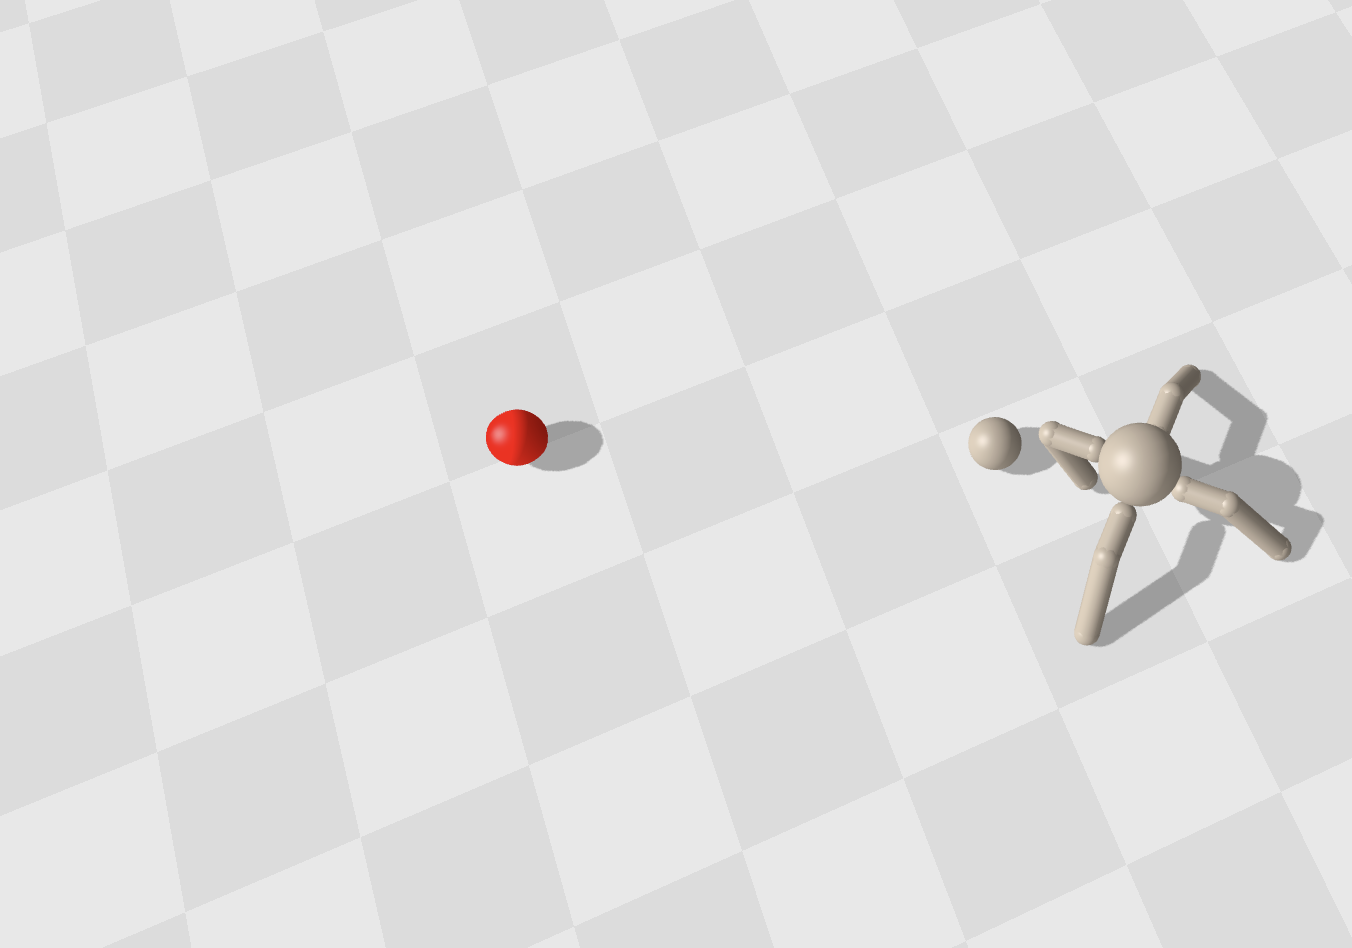
\includegraphics[width=0.33\textwidth]{Bilder/baseline_env} & 
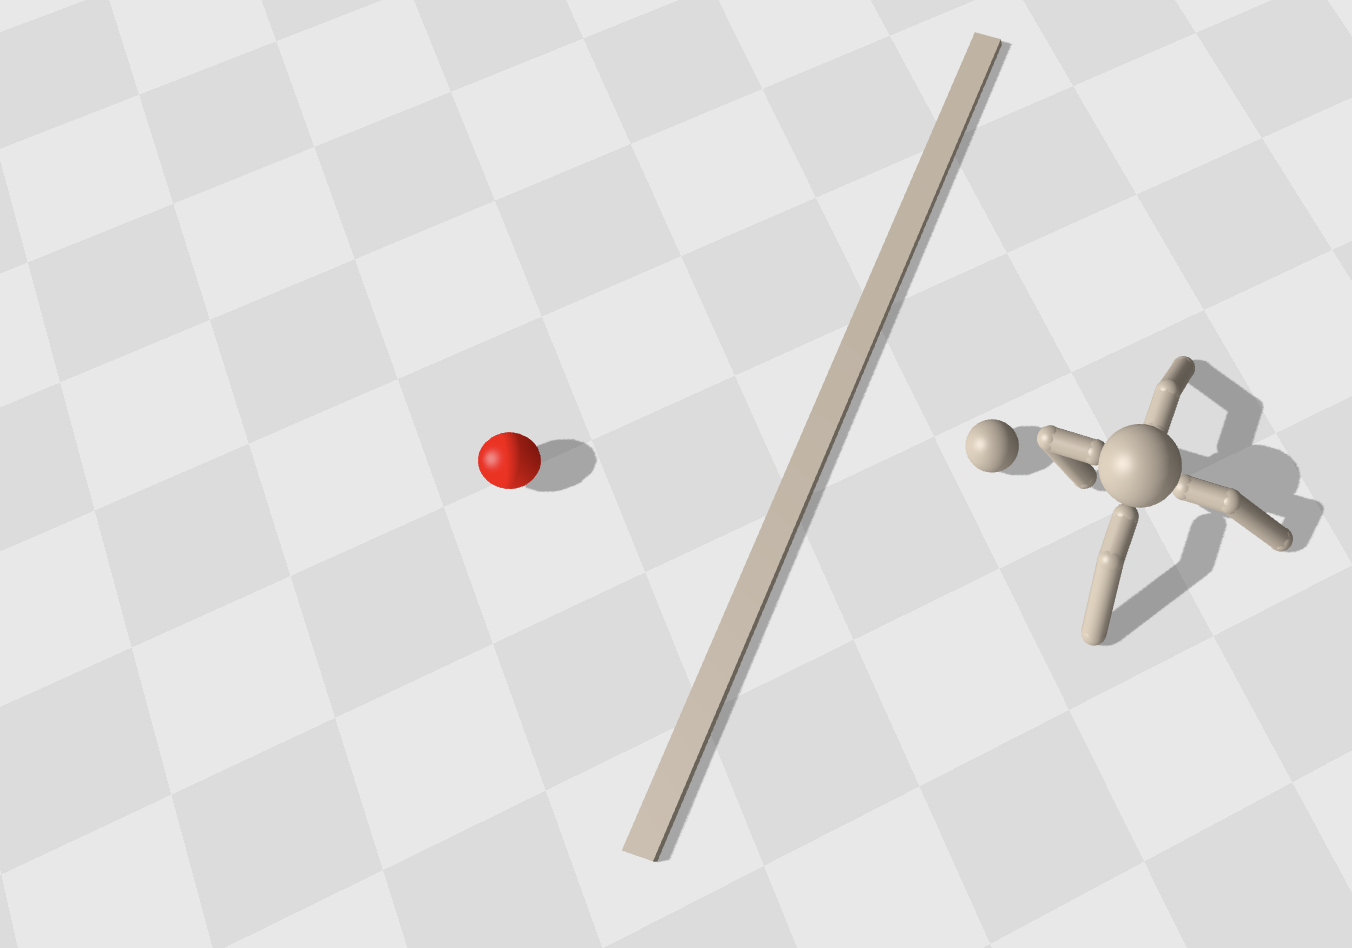
\includegraphics[width=0.33\textwidth]{Bilder/obstacle_env} & 
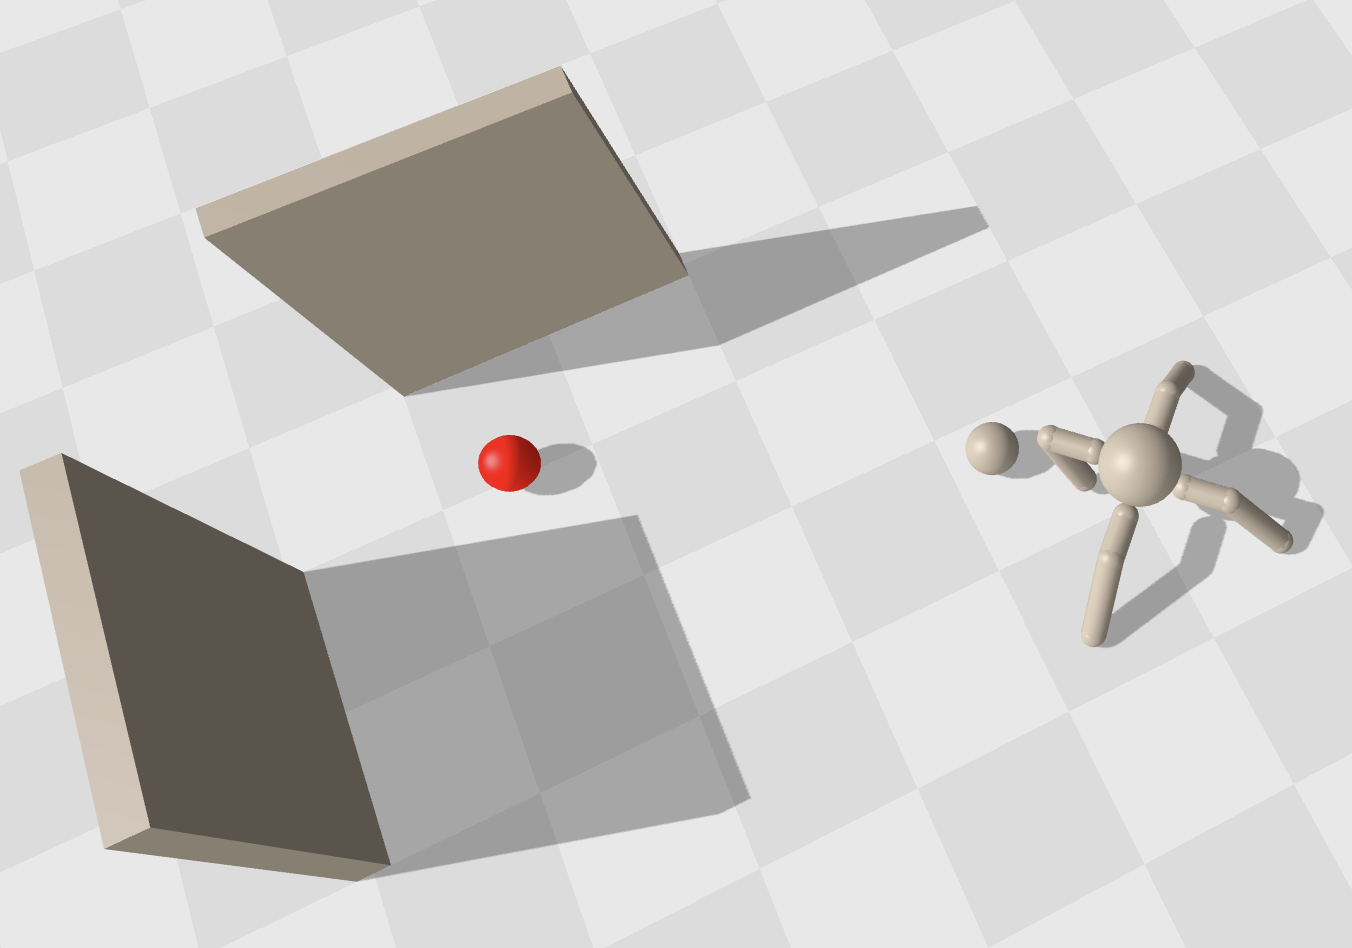
\includegraphics[width=0.33\textwidth]{Bilder/walls_env} \\
(a) Baseline Environment & (b) Obstacle Environment & (c) Walls Environment \\
\end{tabular}
\caption{Visualization of different environments used in the experiments.}
\label{fig:env_images}
\end{table}

\section{Visualization of Minimum Distances for the Environments with Friction Changes} \label{appendix:vis}

\begin{table}[H]
    \centering
    \begin{tabular}{ccccc}
        \begin{subfigure}{0.18\textwidth}
            \centering
            
\includegraphics[width=\linewidth]{0.0}
            \caption{Friction 0.0}
        \end{subfigure} &
        \begin{subfigure}{0.18\textwidth}
            \centering
            
\includegraphics[width=\linewidth]{0.1}
            \caption{Friction 0.1}
        \end{subfigure} &
        \begin{subfigure}{0.18\textwidth}
            \centering
            
\includegraphics[width=\linewidth]{0.2}
            \caption{Friction 0.2}
        \end{subfigure} &
        \begin{subfigure}{0.18\textwidth}
            \centering
            
\includegraphics[width=\linewidth]{0.3}
            \caption{Friction 0.3}
        \end{subfigure} &
        \begin{subfigure}{0.18\textwidth}
            \centering
            
\includegraphics[width=\linewidth]{0.4}
            \caption{Friction 0.4}
        \end{subfigure} \\
        
        \begin{subfigure}{0.18\textwidth}
            \centering
            
\includegraphics[width=\linewidth]{0.5}
            \caption{Friction 0.5}
        \end{subfigure} &
        \begin{subfigure}{0.18\textwidth}
            \centering
            
\includegraphics[width=\linewidth]{0.6}
            \caption{Friction 0.6}
        \end{subfigure} &
        \begin{subfigure}{0.18\textwidth}
            \centering
            
\includegraphics[width=\linewidth]{0.7}
            \caption{Friction 0.7}
        \end{subfigure} &
        \begin{subfigure}{0.18\textwidth}
            \centering
            
\includegraphics[width=\linewidth]{0.8}
            \caption{Friction 0.8}
        \end{subfigure} &
        \begin{subfigure}{0.18\textwidth}
            \centering
            
\includegraphics[width=\linewidth]{0.9}
            \caption{Friction 0.9}
        \end{subfigure} \\
    \end{tabular}
    \caption{Visualization of minimum distances of the best solutions found in the environments with different friction values.}
    \label{tab:friction_images}
\end{table}
\clearpage

 \section{Adaptation for Different Friction Values} \label{appendix:gp_pred}

\begin{longtable}{@{}c@{}c@{}}
    \begin{minipage}[c]{0.5\linewidth}  % Changed [t] to [c] for vertical centering
        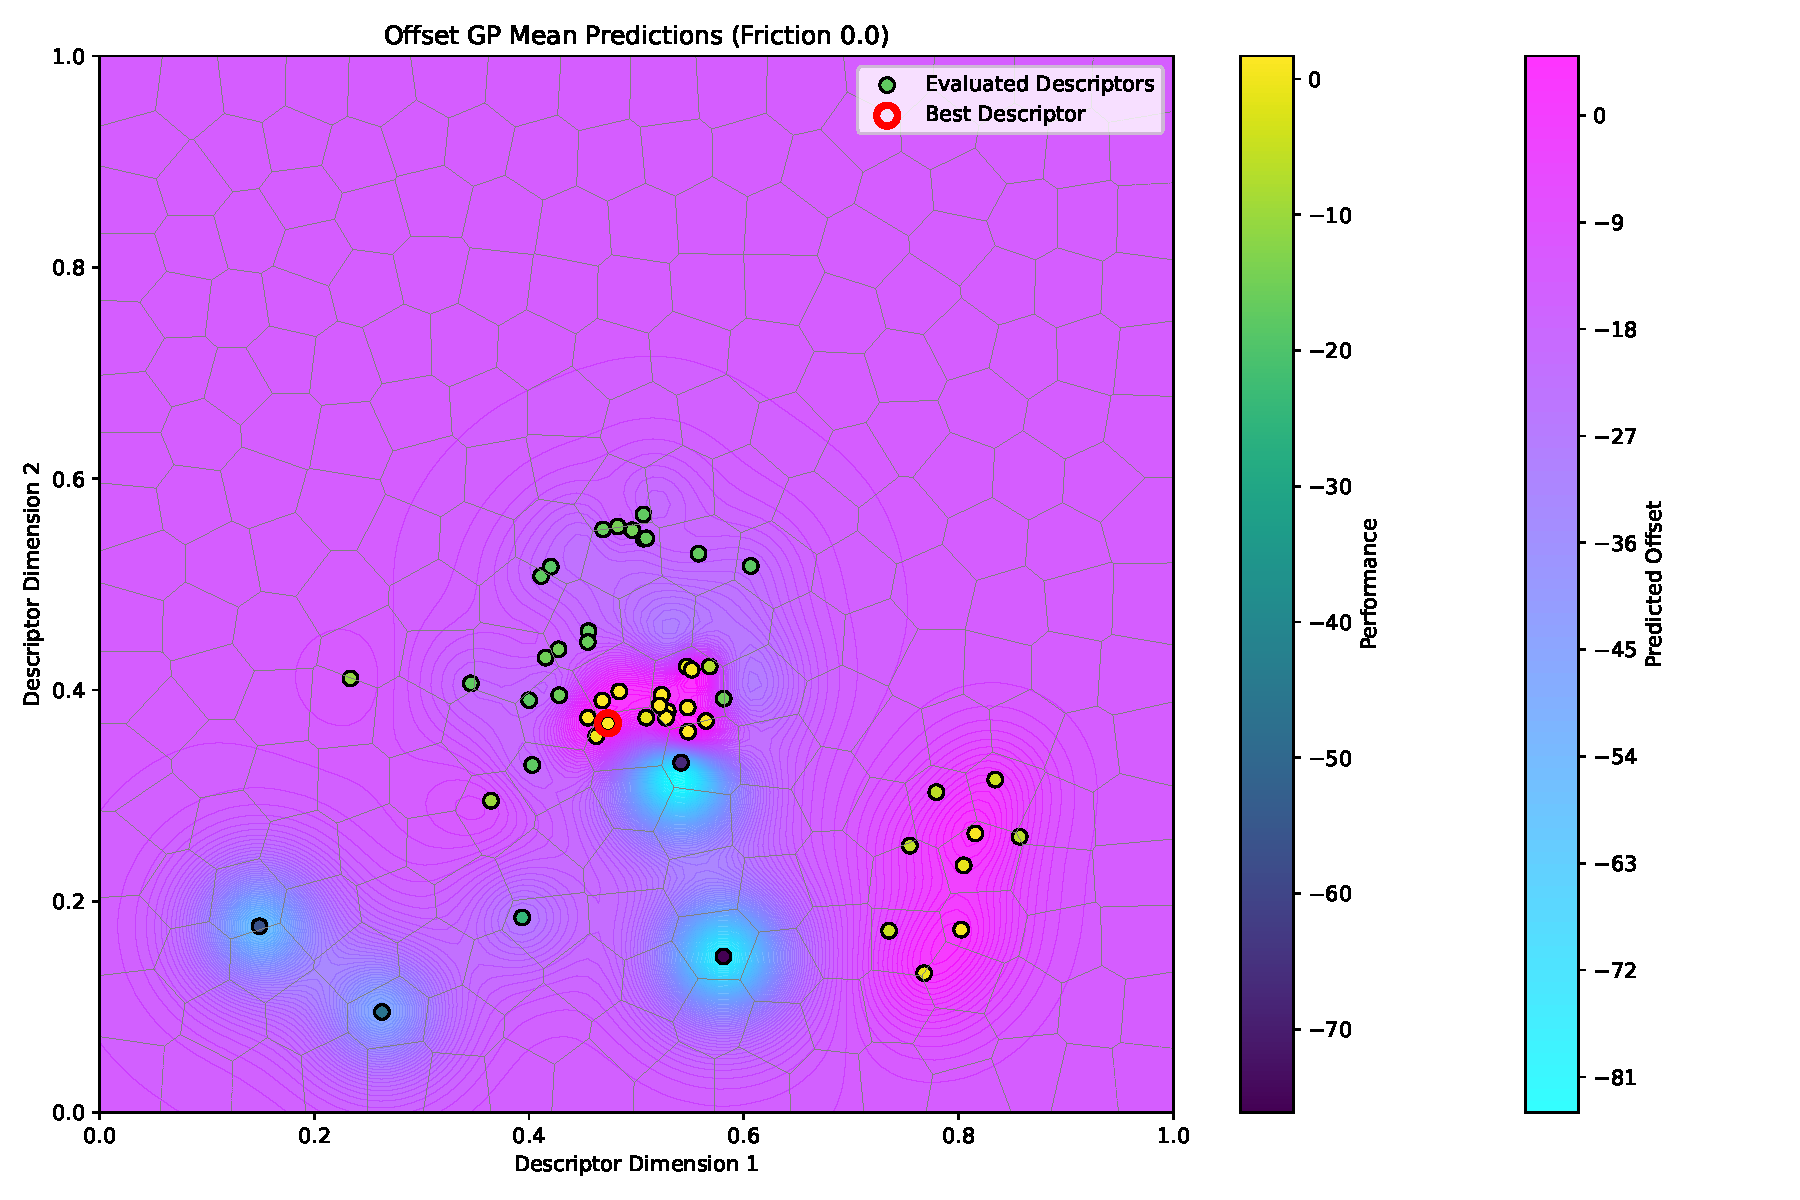
\includegraphics[width=\linewidth]{Bilder/appendix/omp_0.0.pdf}
    \end{minipage} &
    \begin{minipage}[c]{0.5\linewidth}  % Changed [t] to [c] for vertical centering
        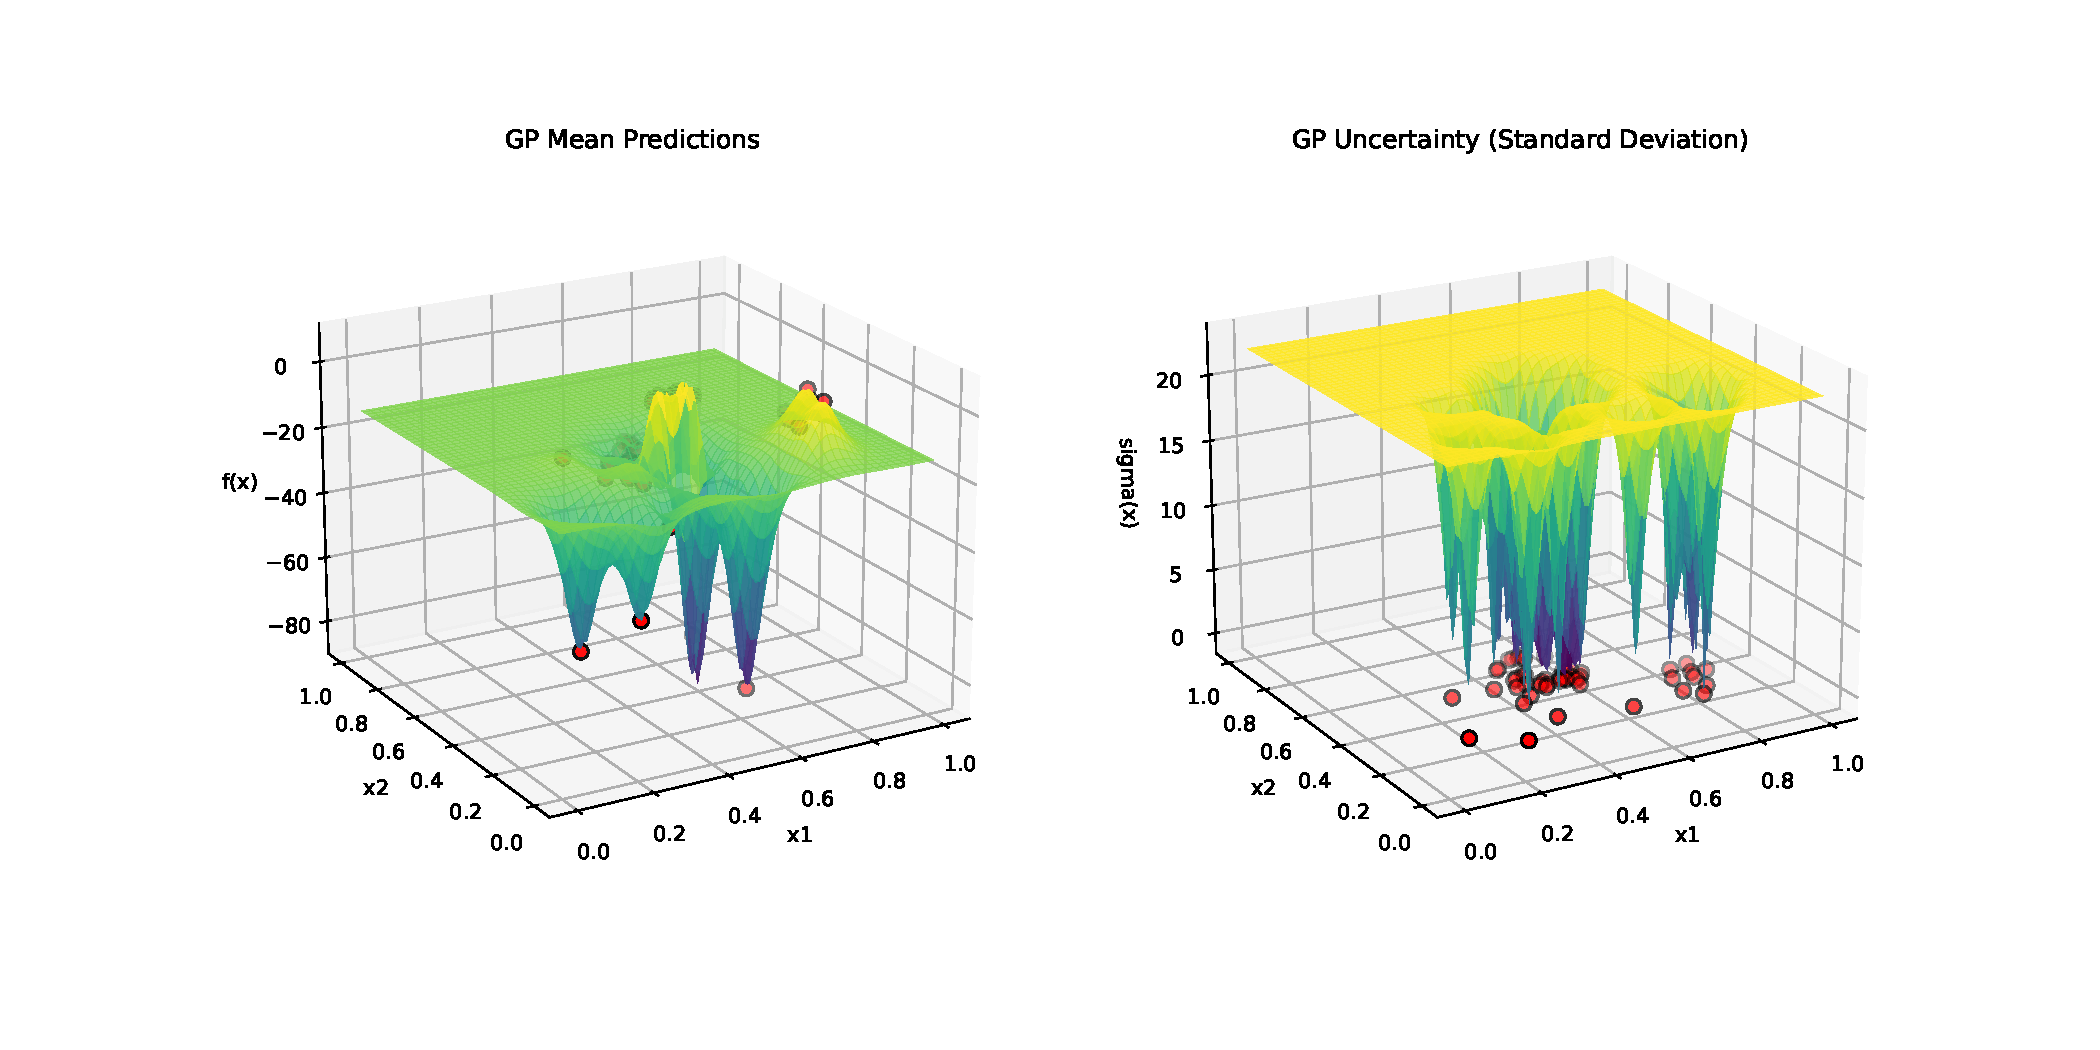
\includegraphics[width=\linewidth]{Bilder/appendix/3D_omp_0.0.pdf}
    \end{minipage} \\
    \begin{minipage}[c]{0.5\linewidth}
        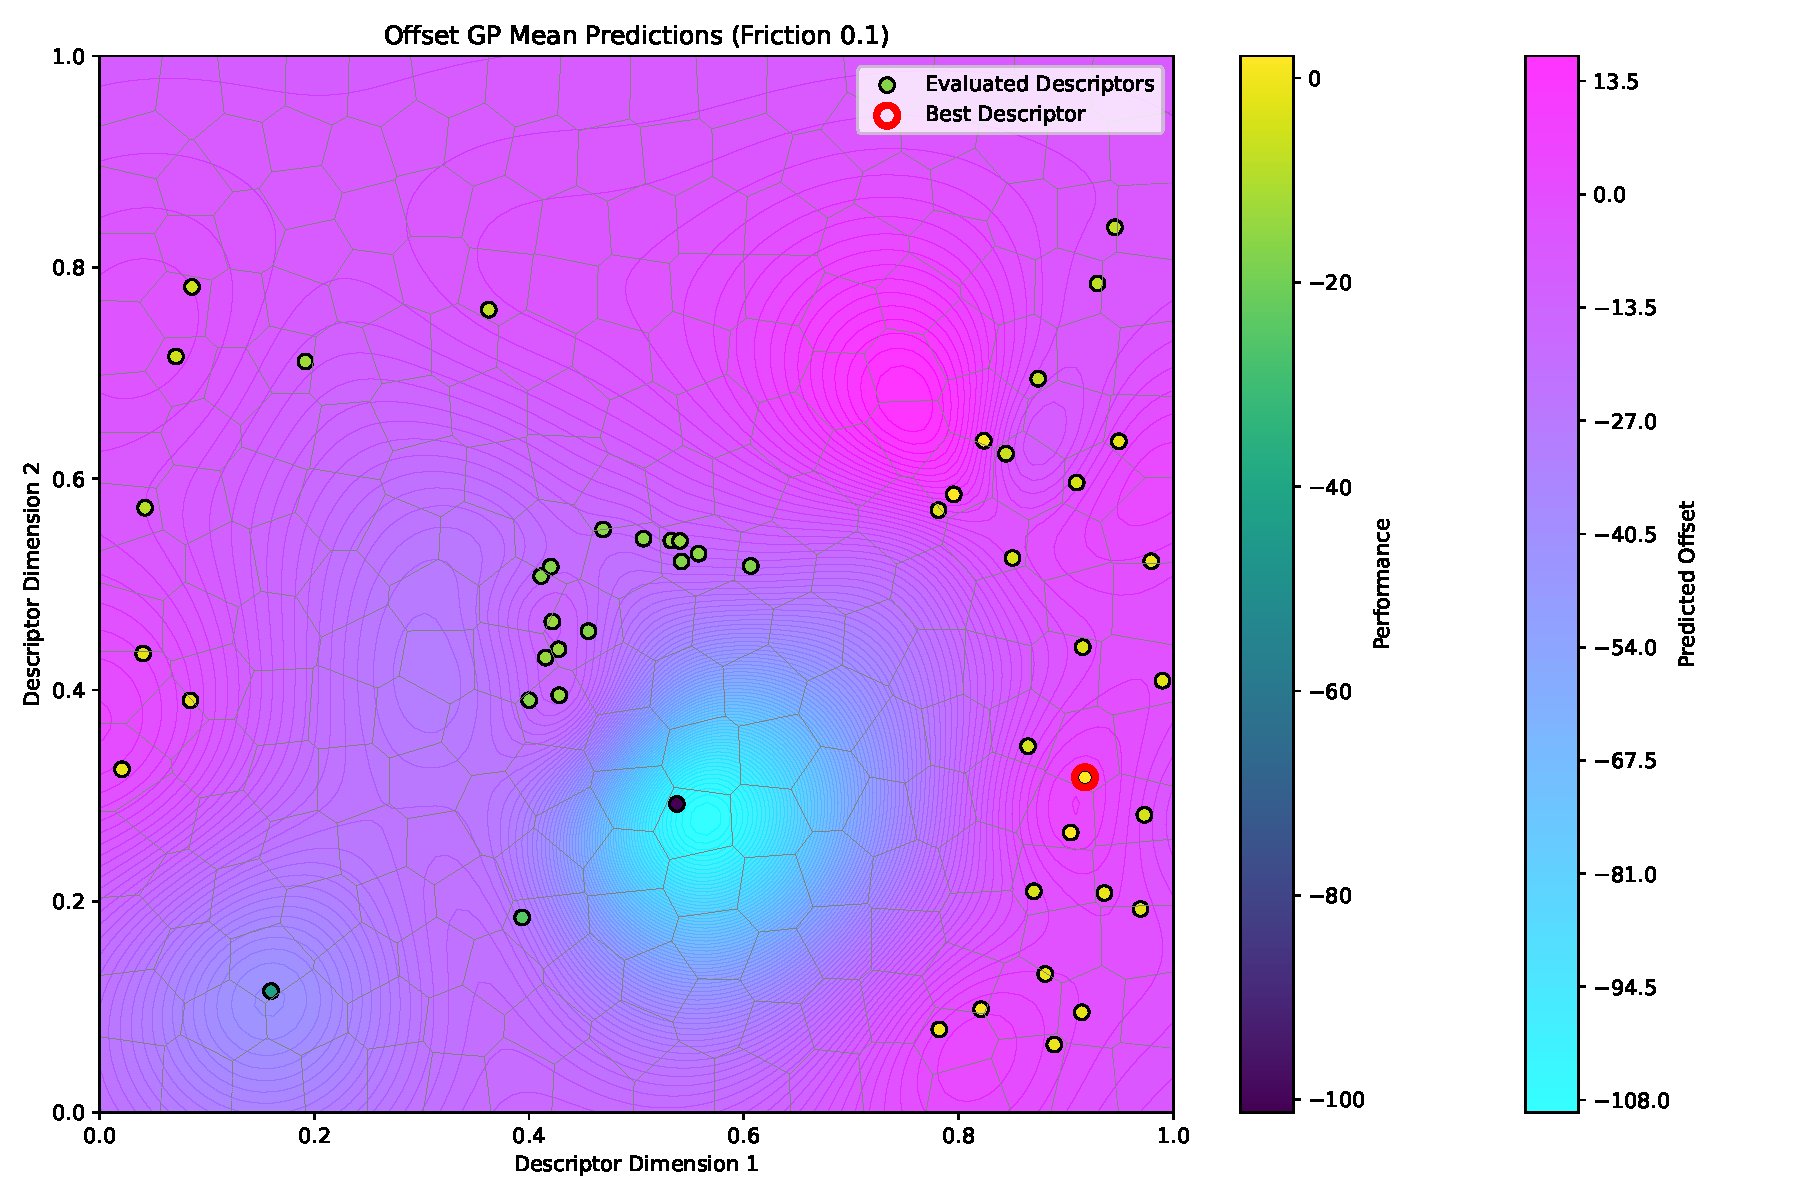
\includegraphics[width=\linewidth]{Bilder/appendix/omp_0.1.pdf}
    \end{minipage} &
    \begin{minipage}[c]{0.5\linewidth}
        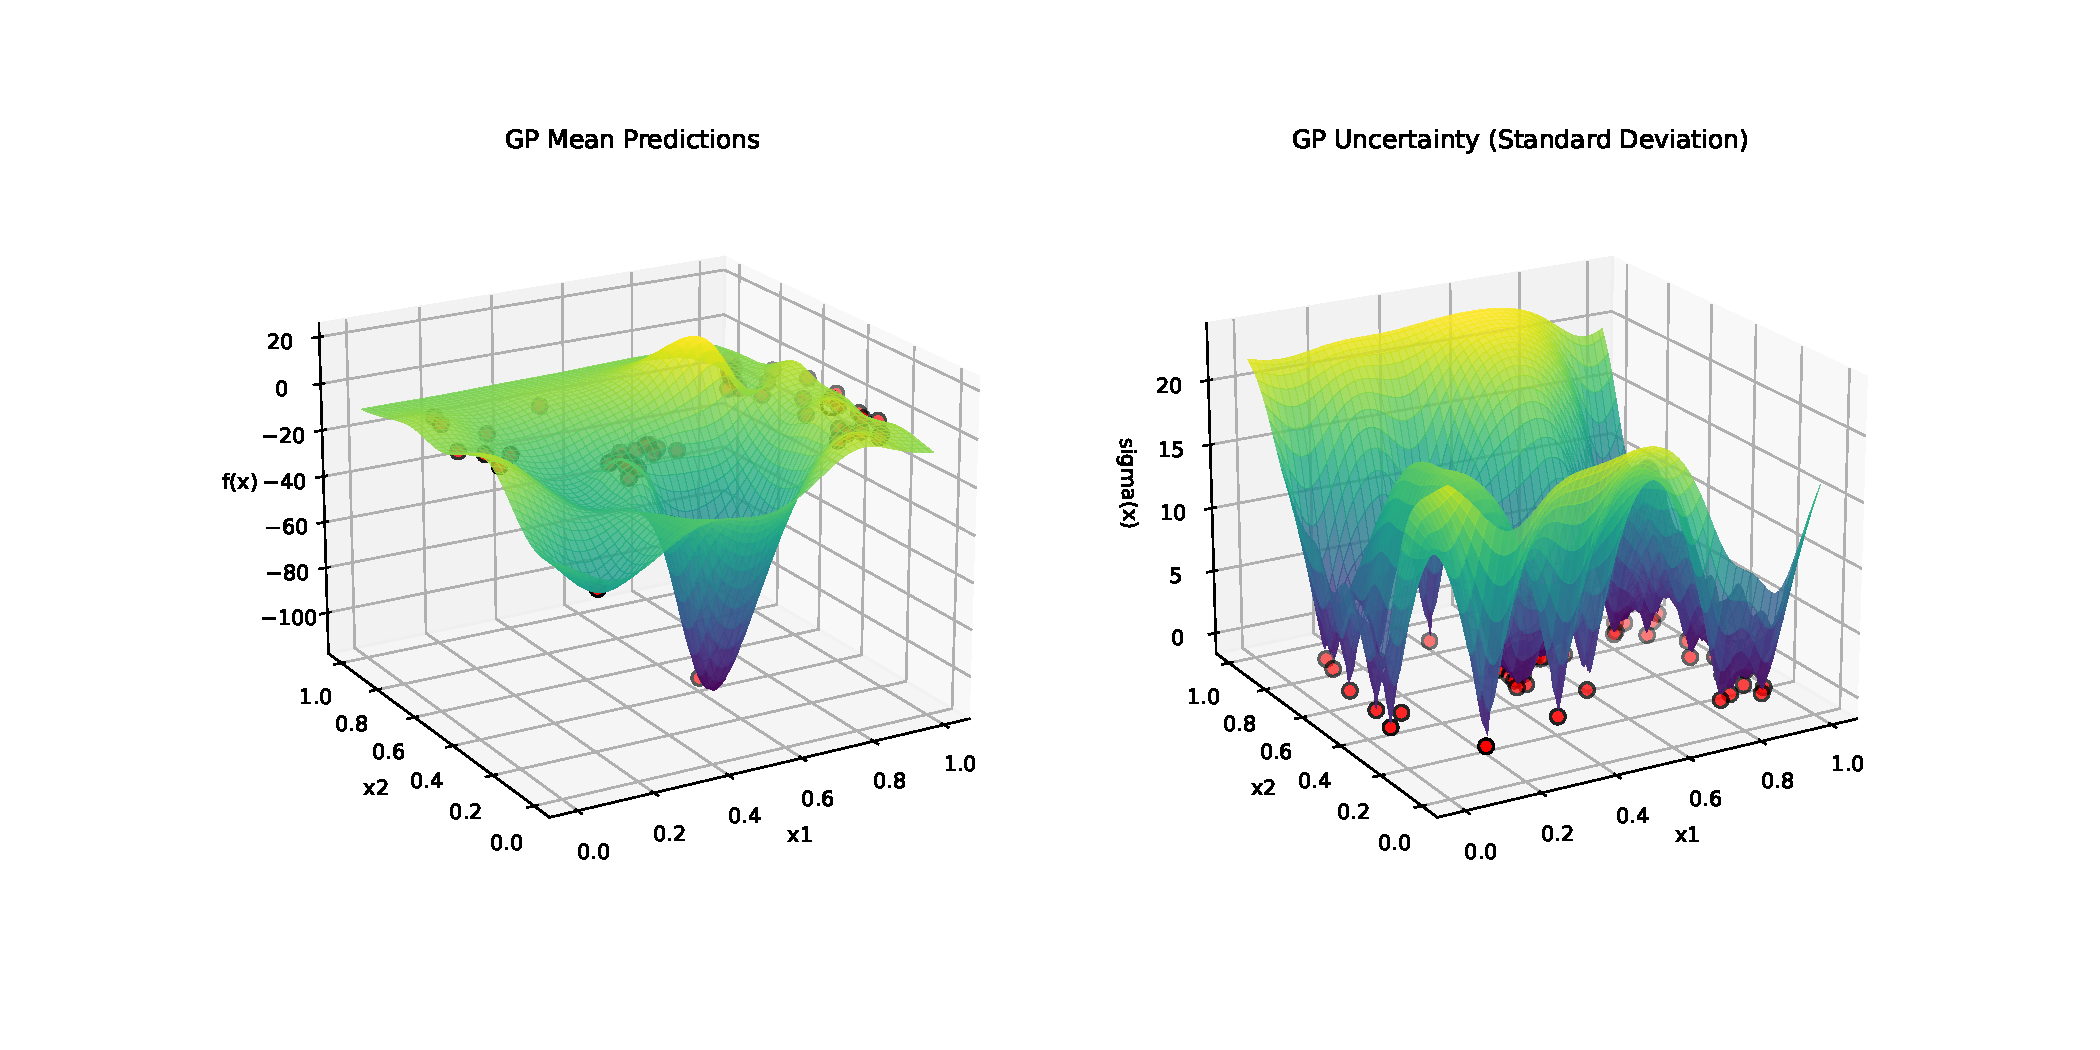
\includegraphics[width=\linewidth]{Bilder/appendix/3D_omp_0.1.pdf}
    \end{minipage} \\
    \begin{minipage}[c]{0.5\linewidth}
        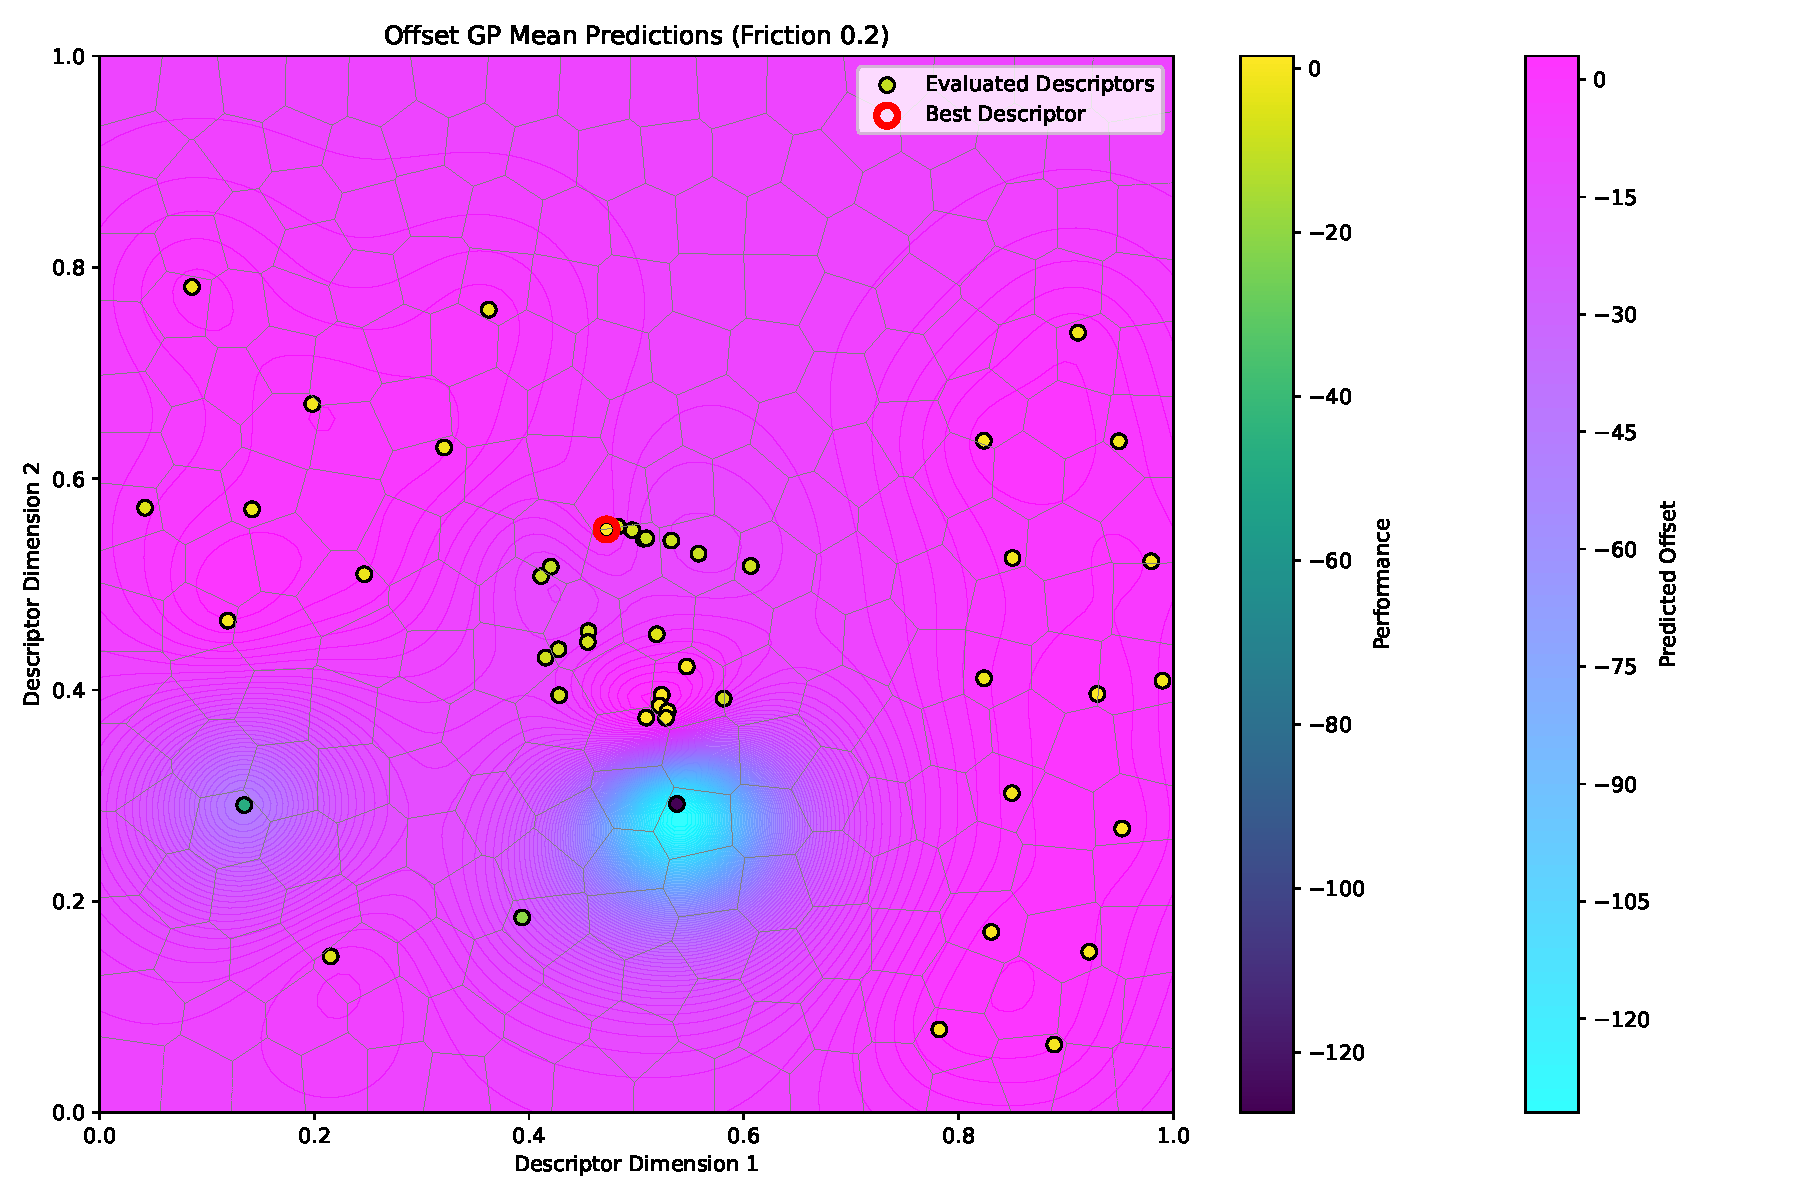
\includegraphics[width=\linewidth]{Bilder/appendix/omp_0.2_.pdf}
    \end{minipage} &
    \begin{minipage}[c]{0.5\linewidth}
        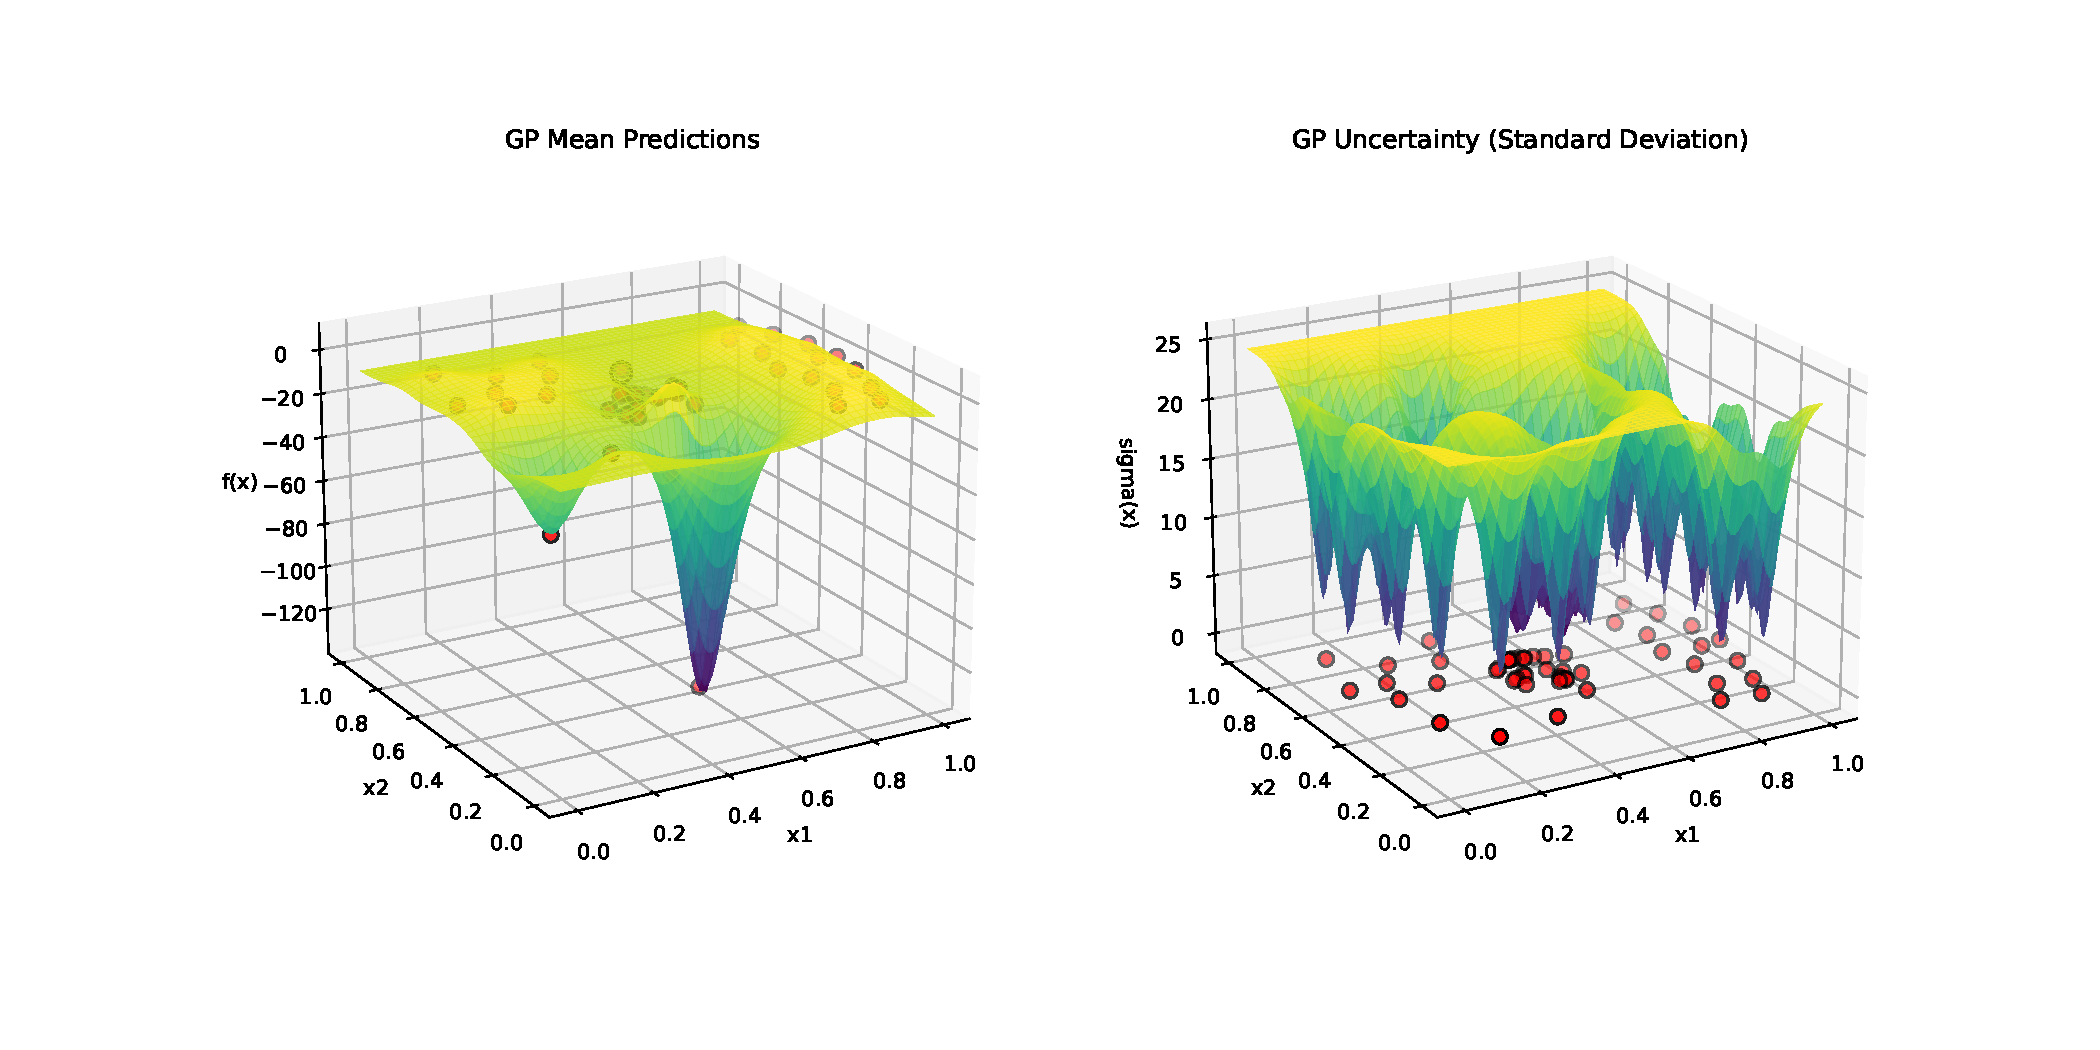
\includegraphics[width=\linewidth]{Bilder/appendix/3D_omp_0.2_.pdf}
    \end{minipage} \\
    \begin{minipage}[c]{0.5\linewidth}
        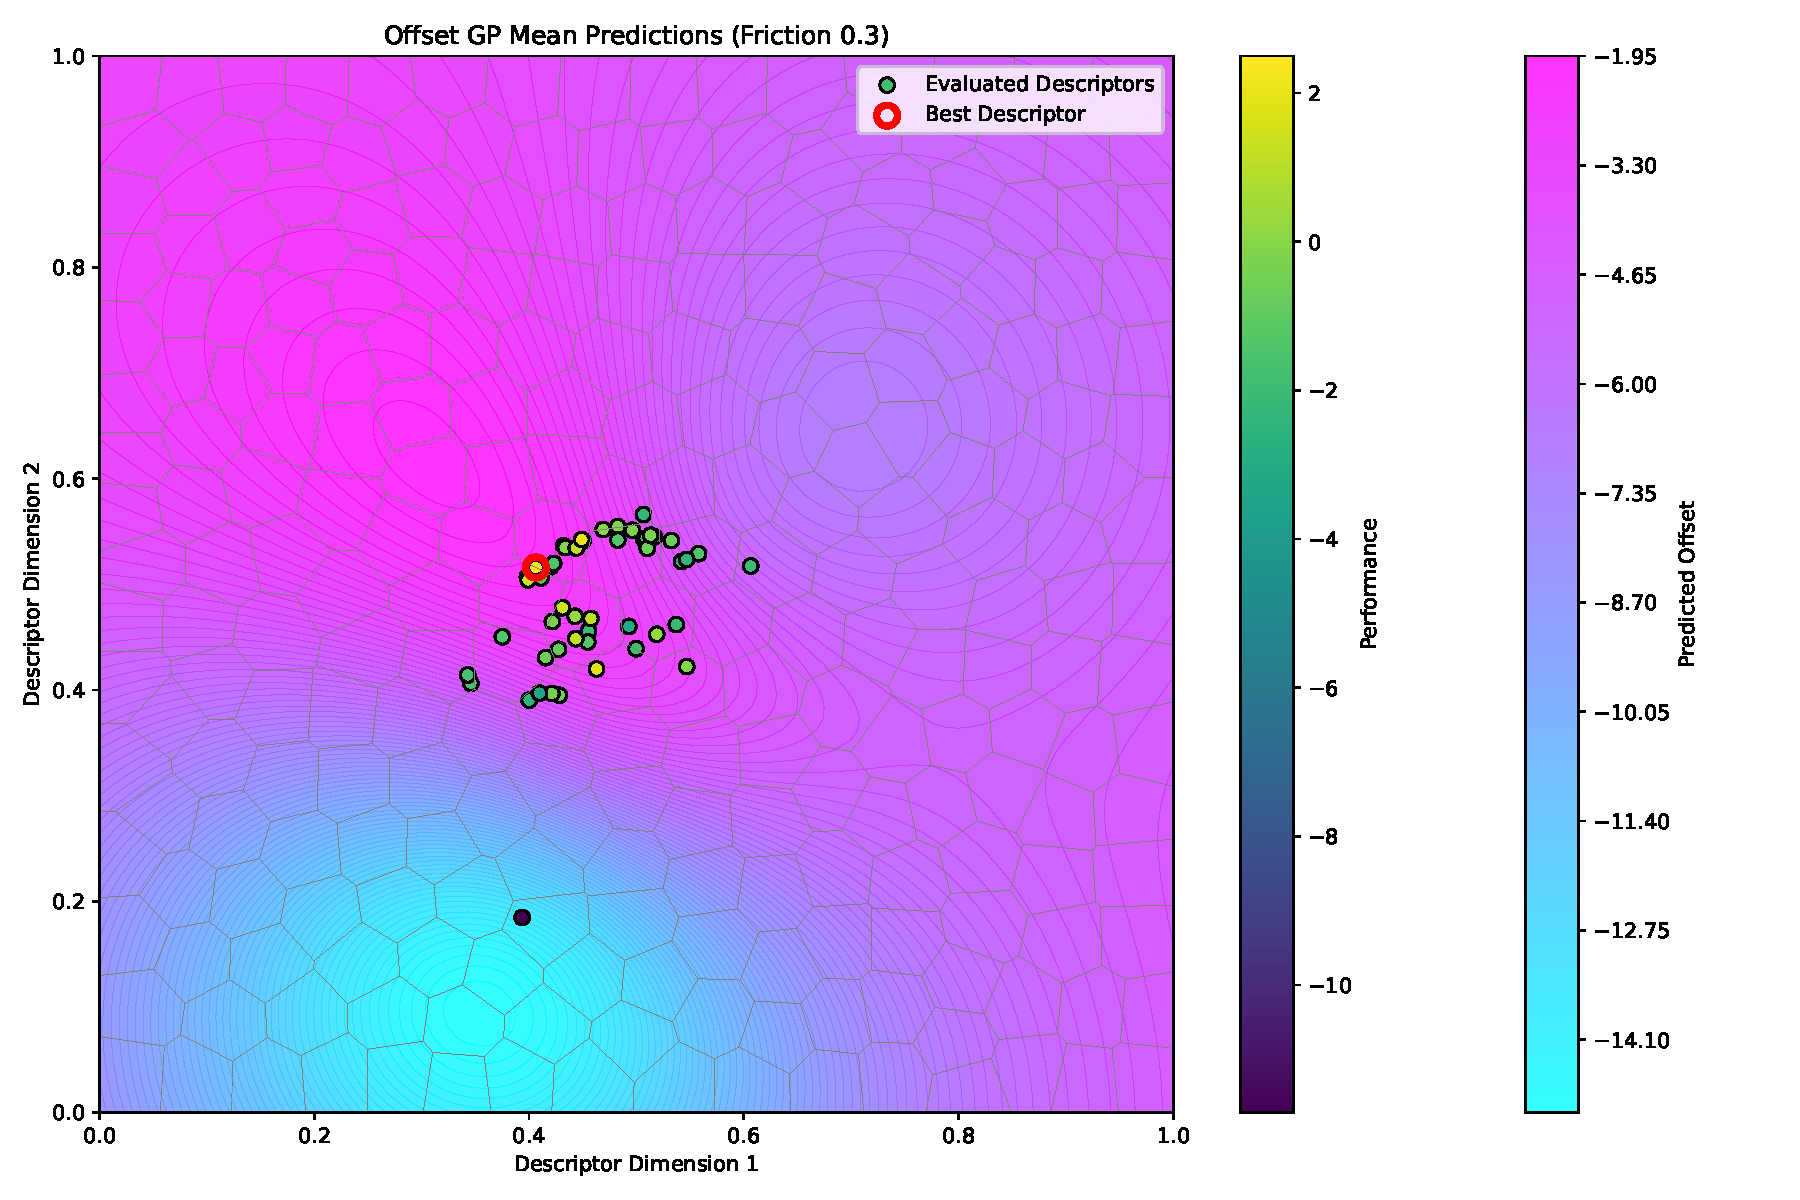
\includegraphics[width=\linewidth]{Bilder/appendix/omp_0.3.pdf}
    \end{minipage} &
    \begin{minipage}[c]{0.5\linewidth}
        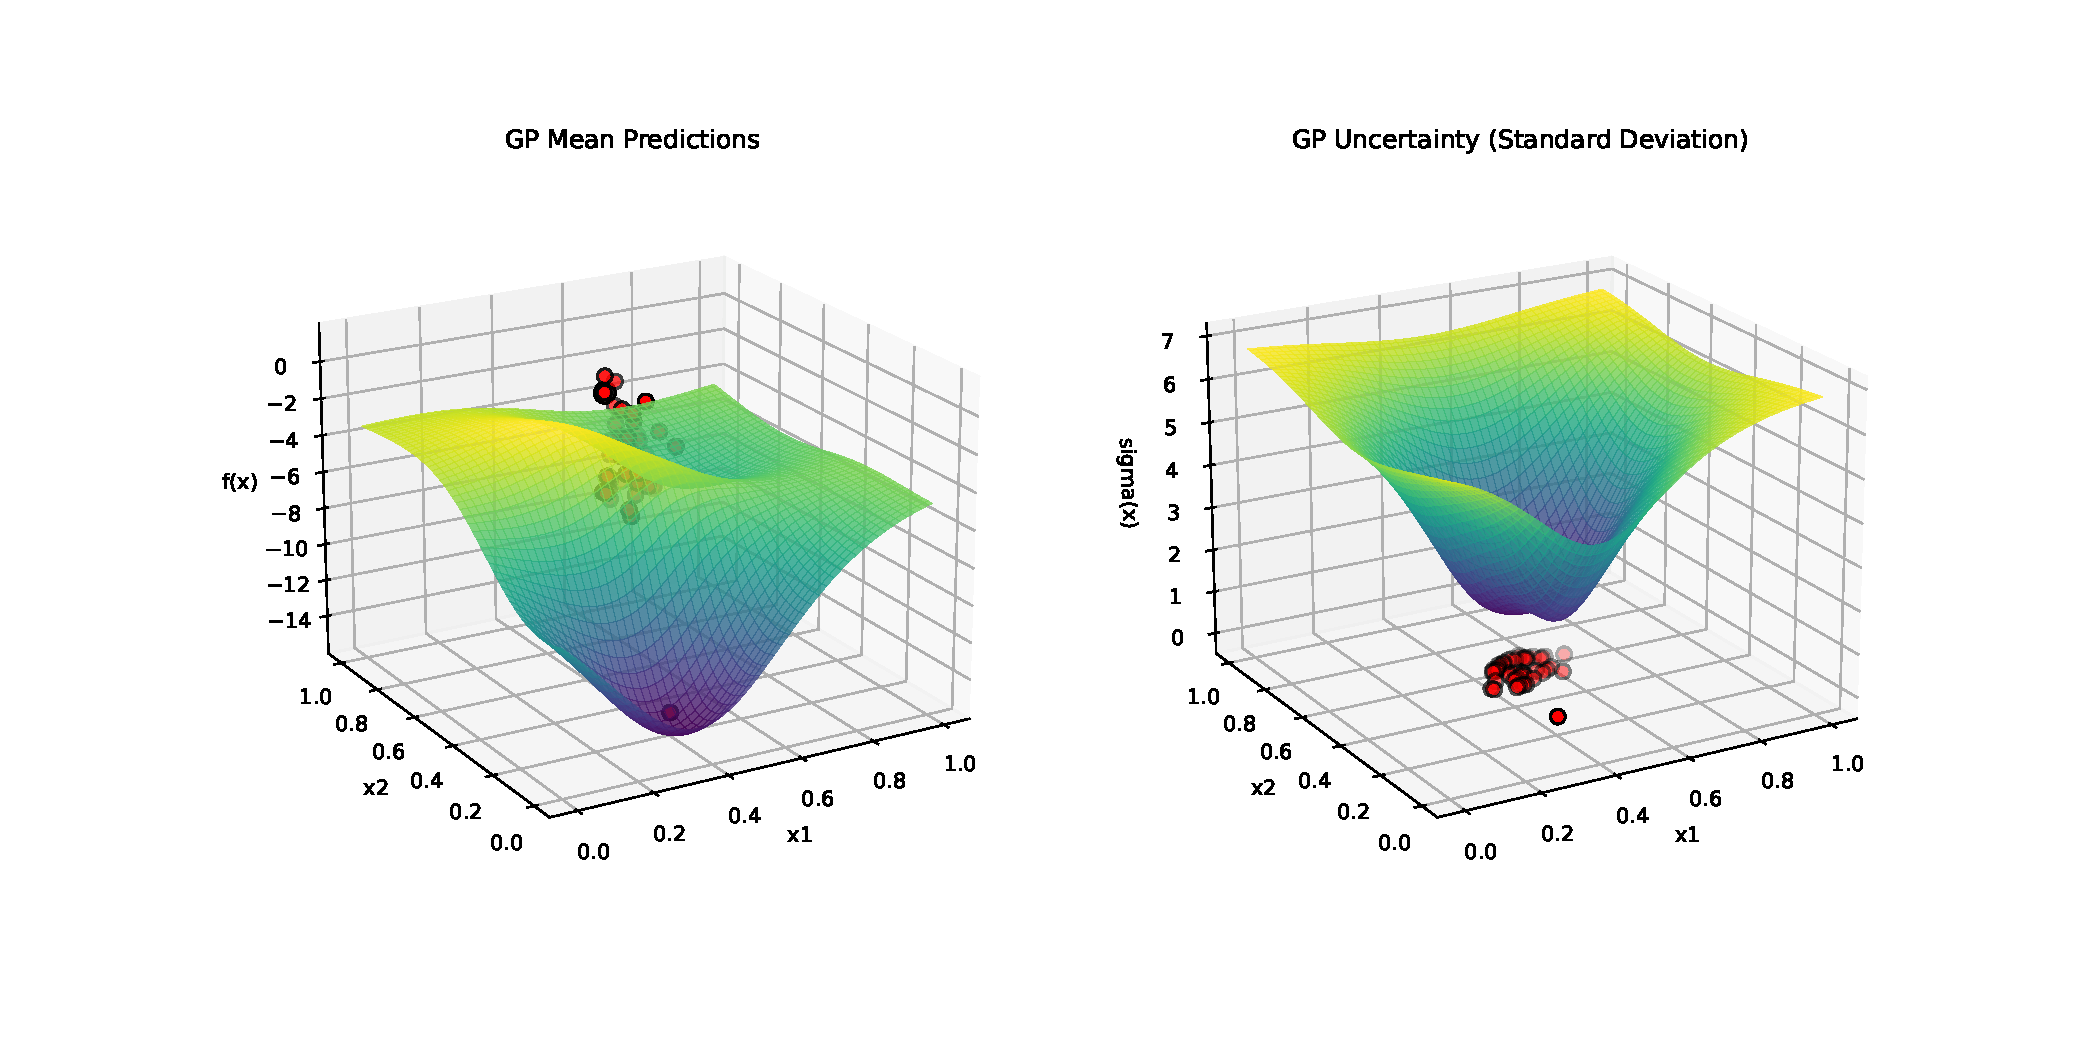
\includegraphics[width=\linewidth]{Bilder/appendix/3D_omp_0.3_.pdf}
    \end{minipage} \\
    \begin{minipage}[c]{0.5\linewidth}
        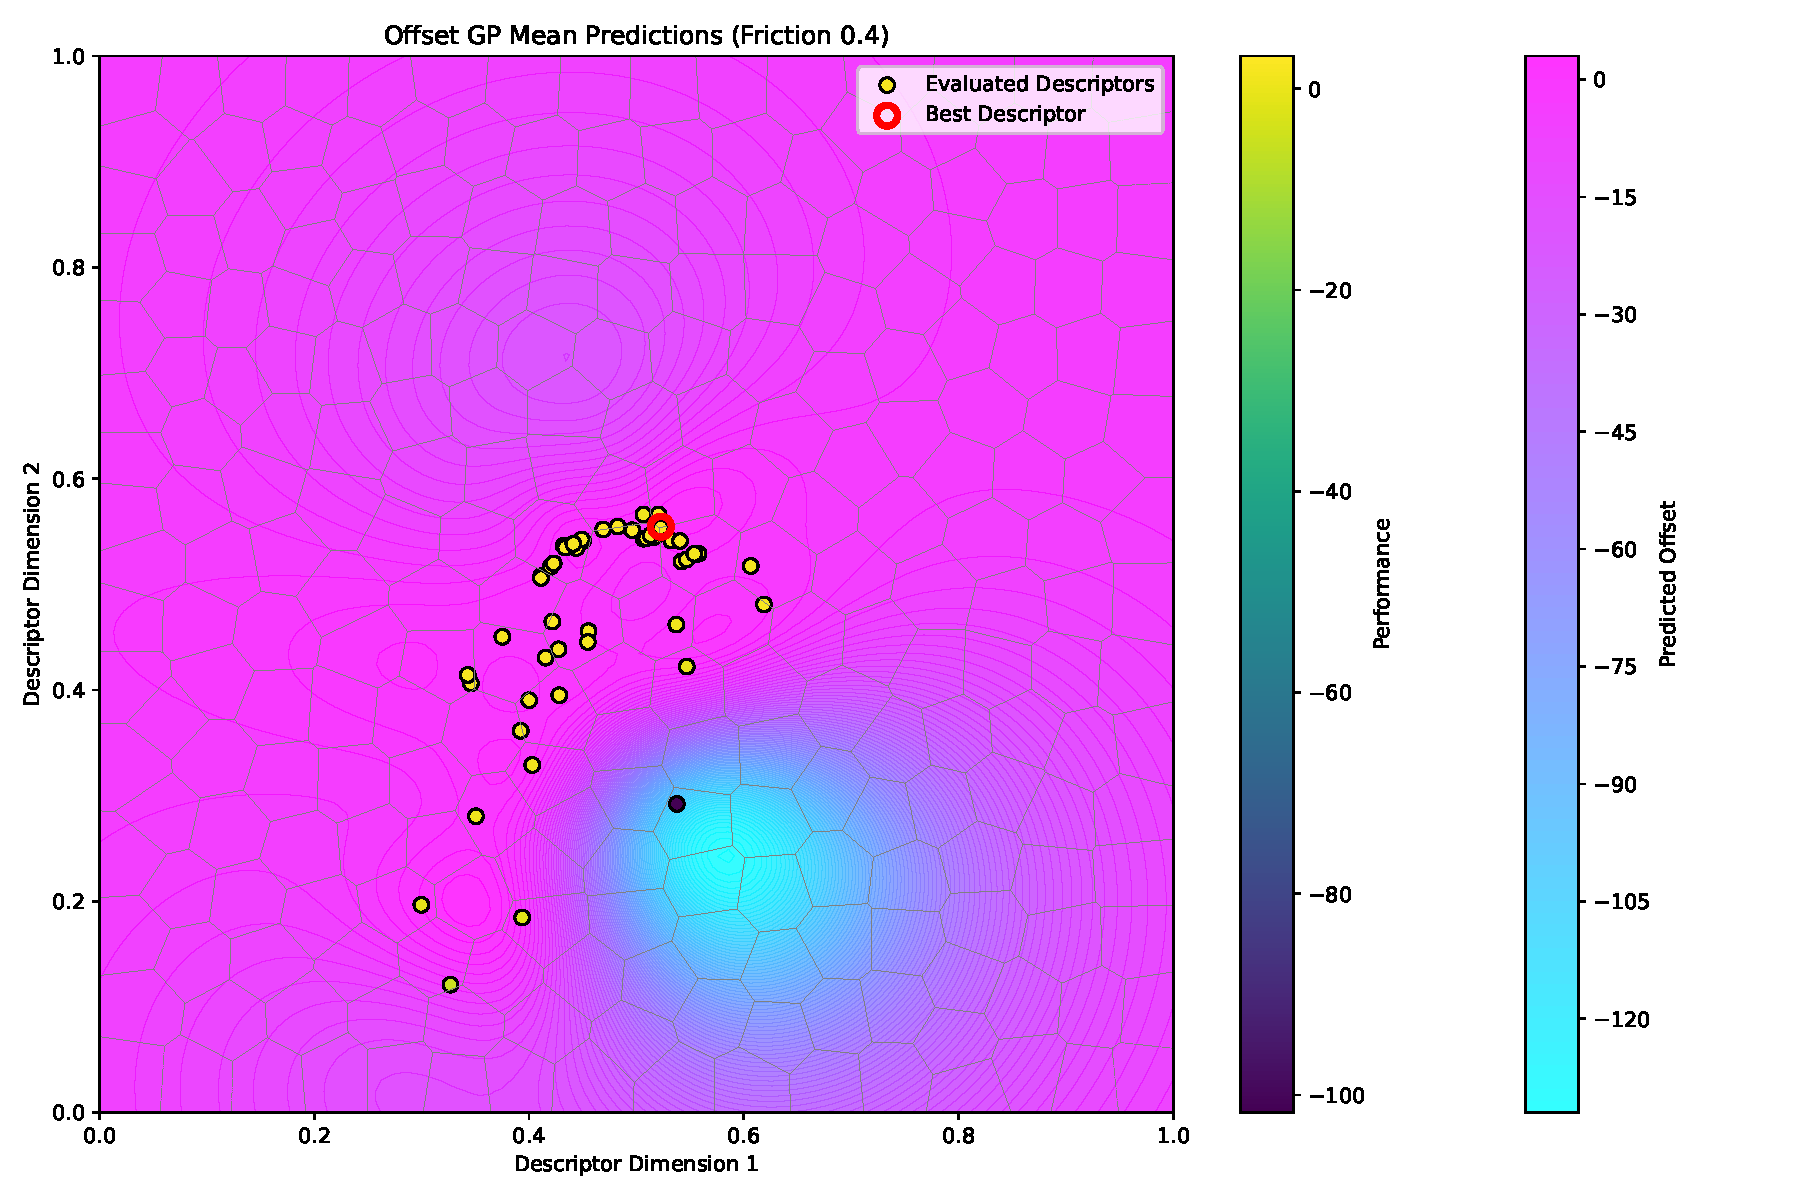
\includegraphics[width=\linewidth]{Bilder/appendix/omp_0.4.pdf}
    \end{minipage} &
    \begin{minipage}[c]{0.5\linewidth}
        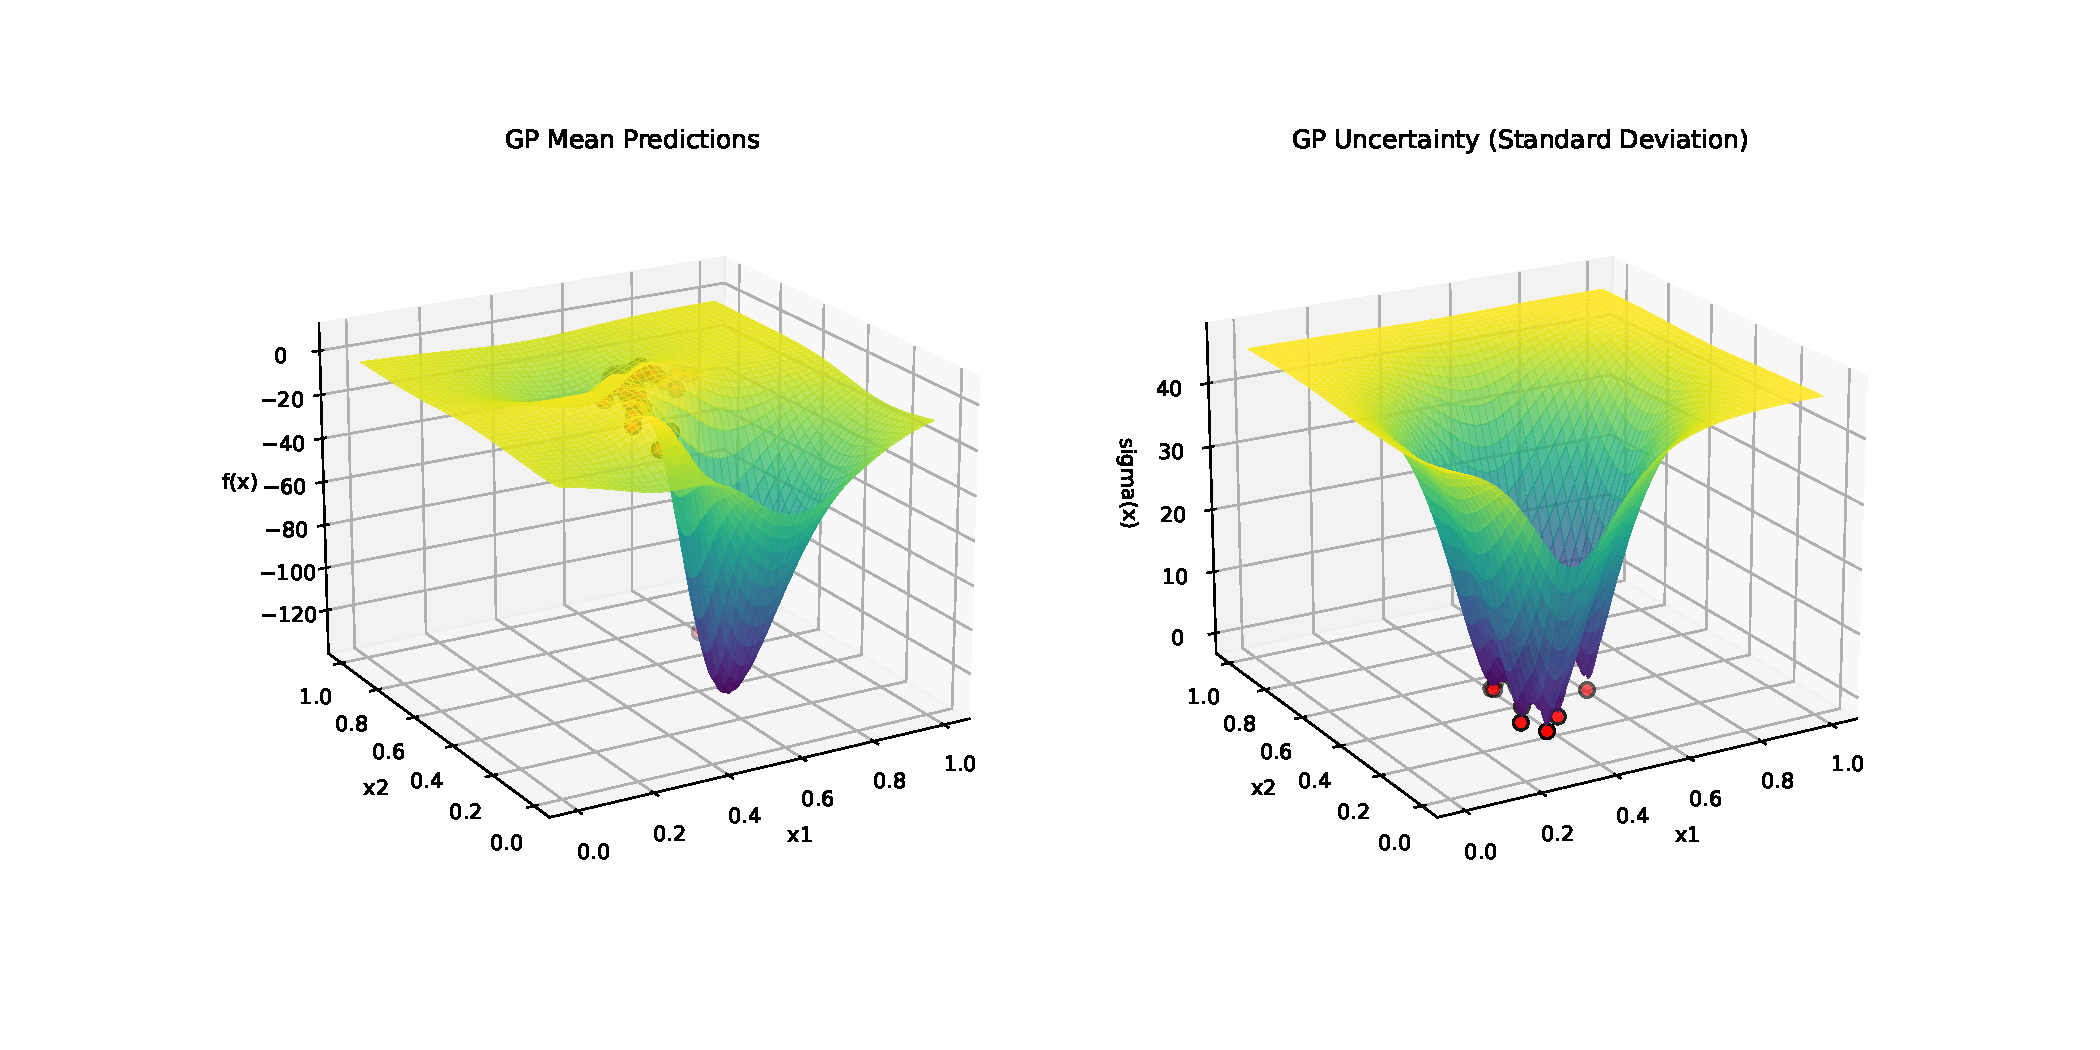
\includegraphics[width=\linewidth]{Bilder/appendix/3D_omp_0.4.pdf}
    \end{minipage} \\
    \begin{minipage}[c]{0.5\linewidth}
        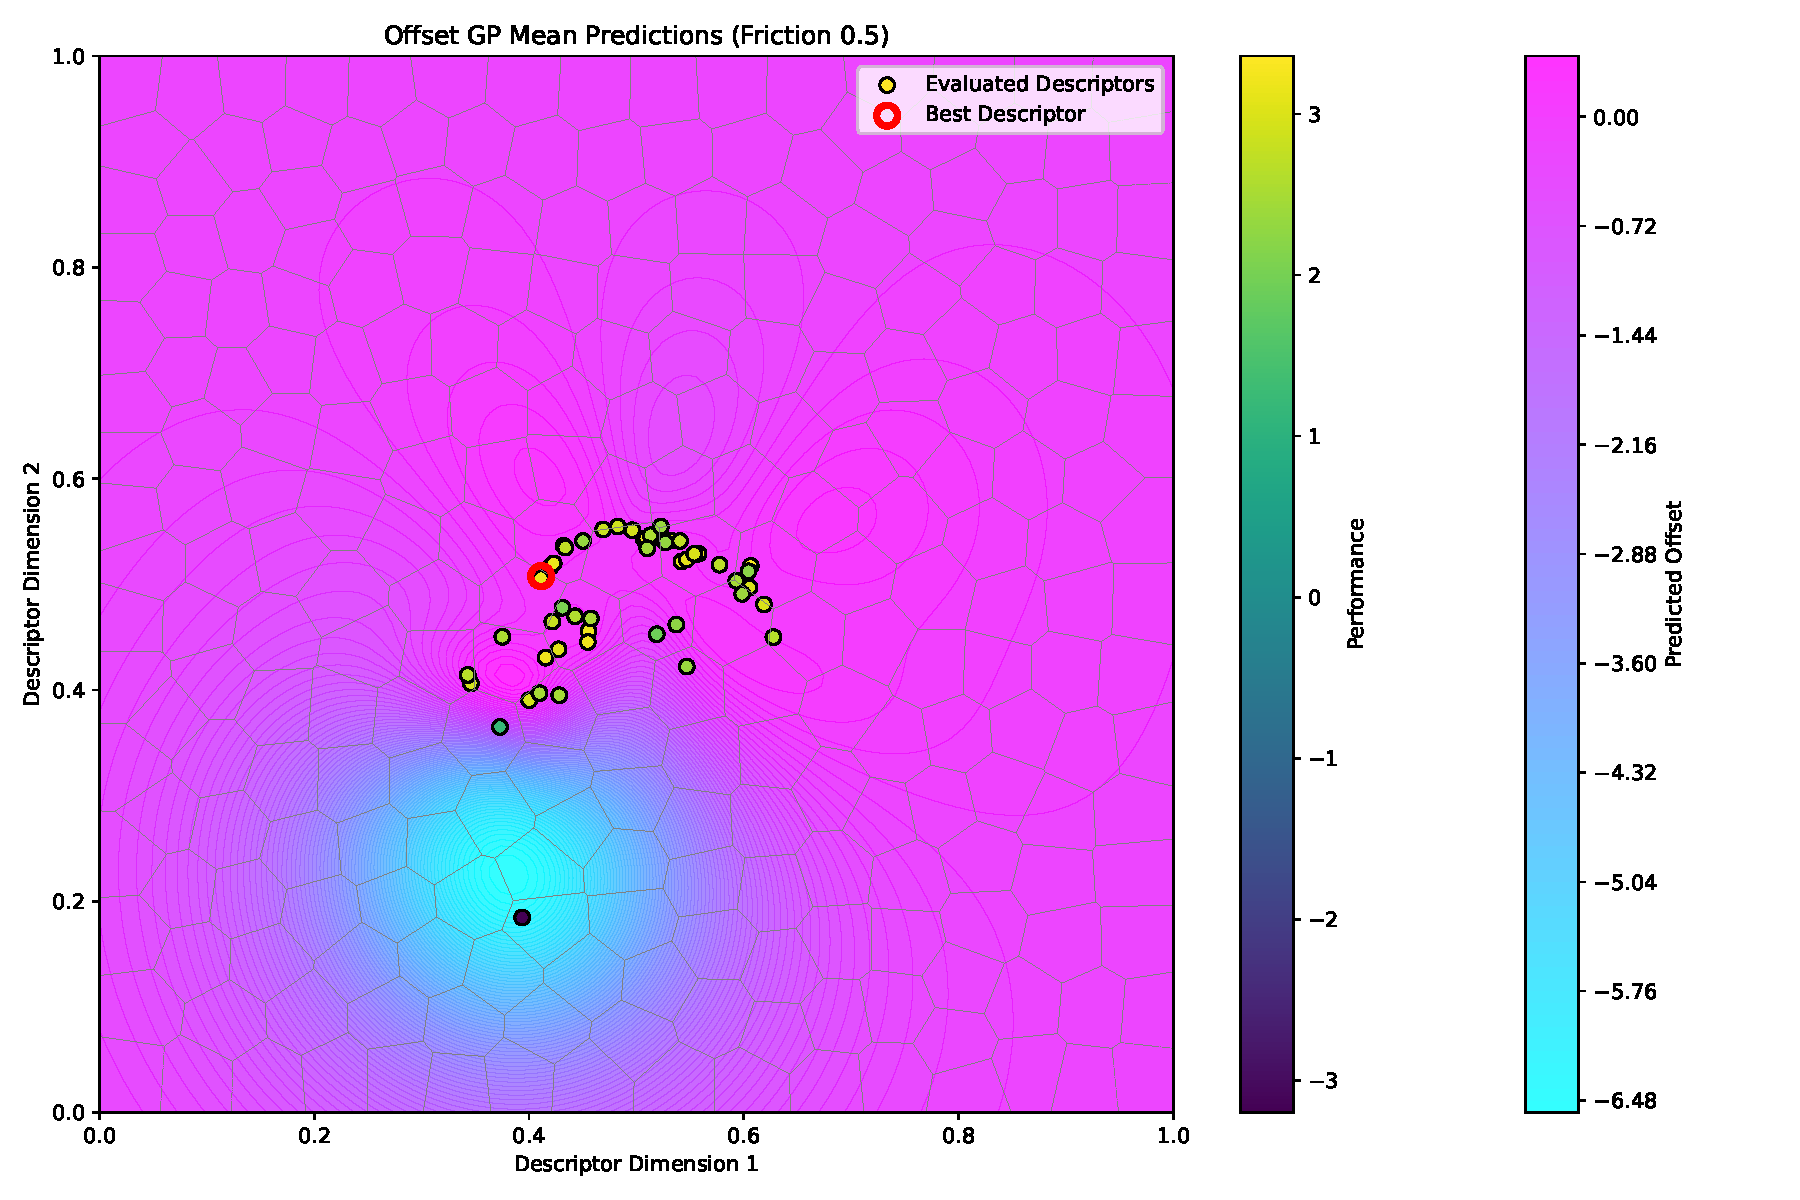
\includegraphics[width=\linewidth]{Bilder/appendix/omp_0.5.pdf}
    \end{minipage} &
    \begin{minipage}[c]{0.5\linewidth}
        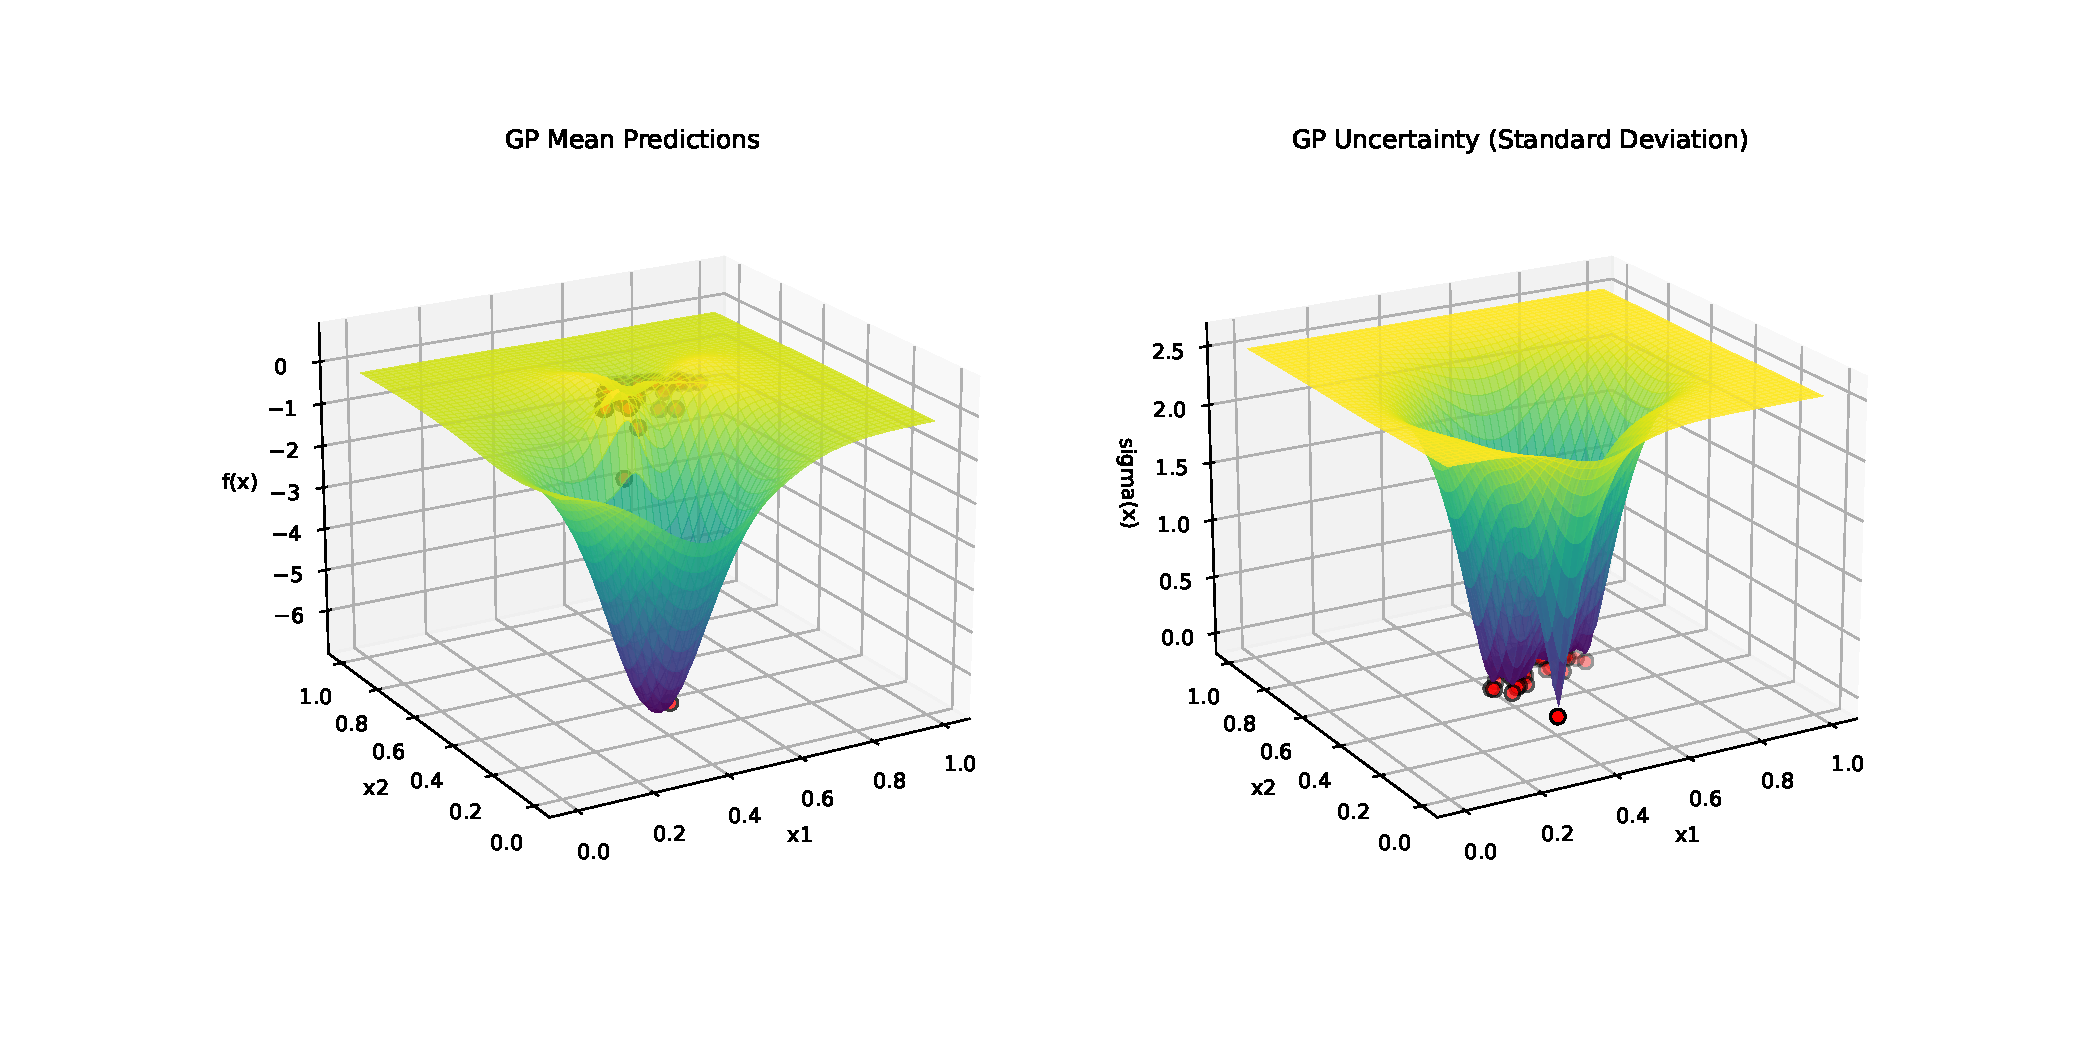
\includegraphics[width=\linewidth]{Bilder/appendix/3D_omp_0.5.pdf}
    \end{minipage} \\
    \begin{minipage}[c]{0.5\linewidth}
        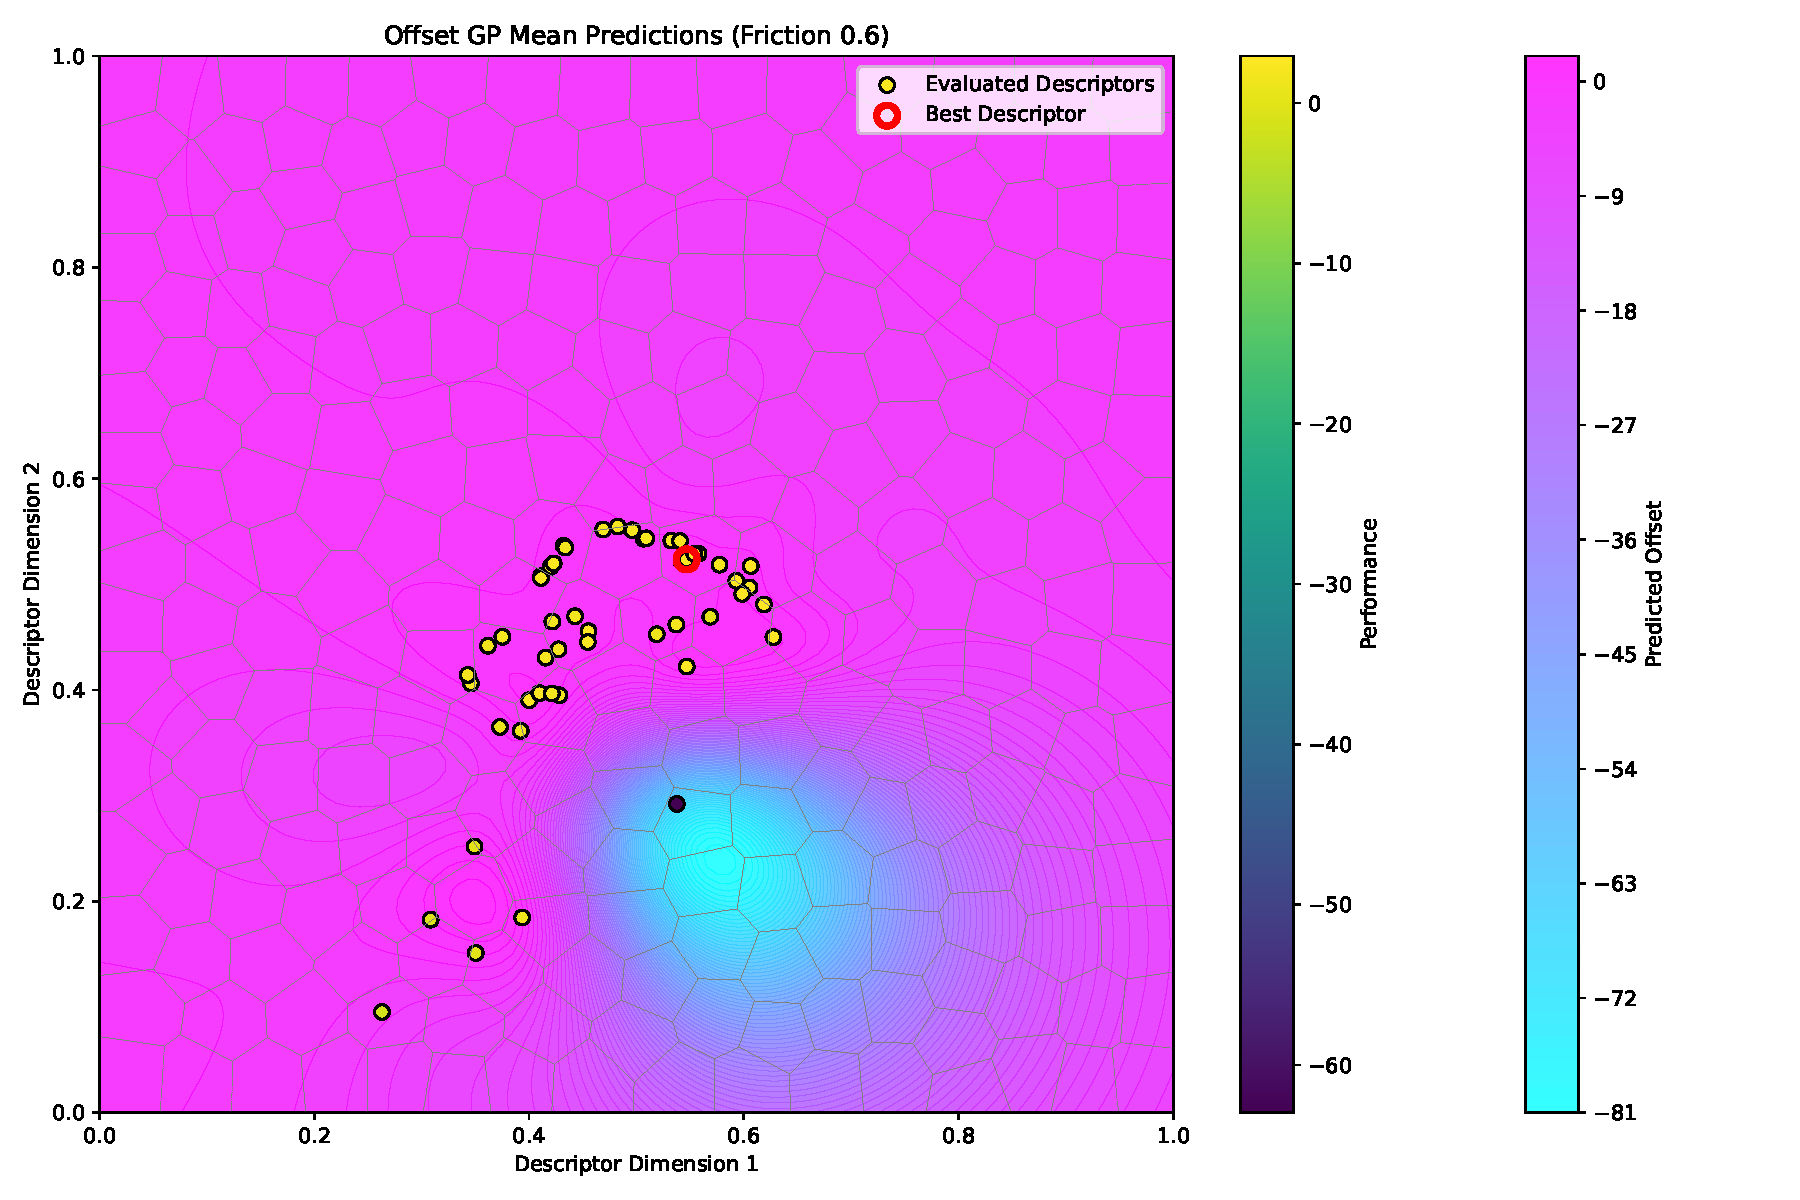
\includegraphics[width=\linewidth]{Bilder/appendix/omp_0.6.pdf}
    \end{minipage} &
    \begin{minipage}[c]{0.5\linewidth}
        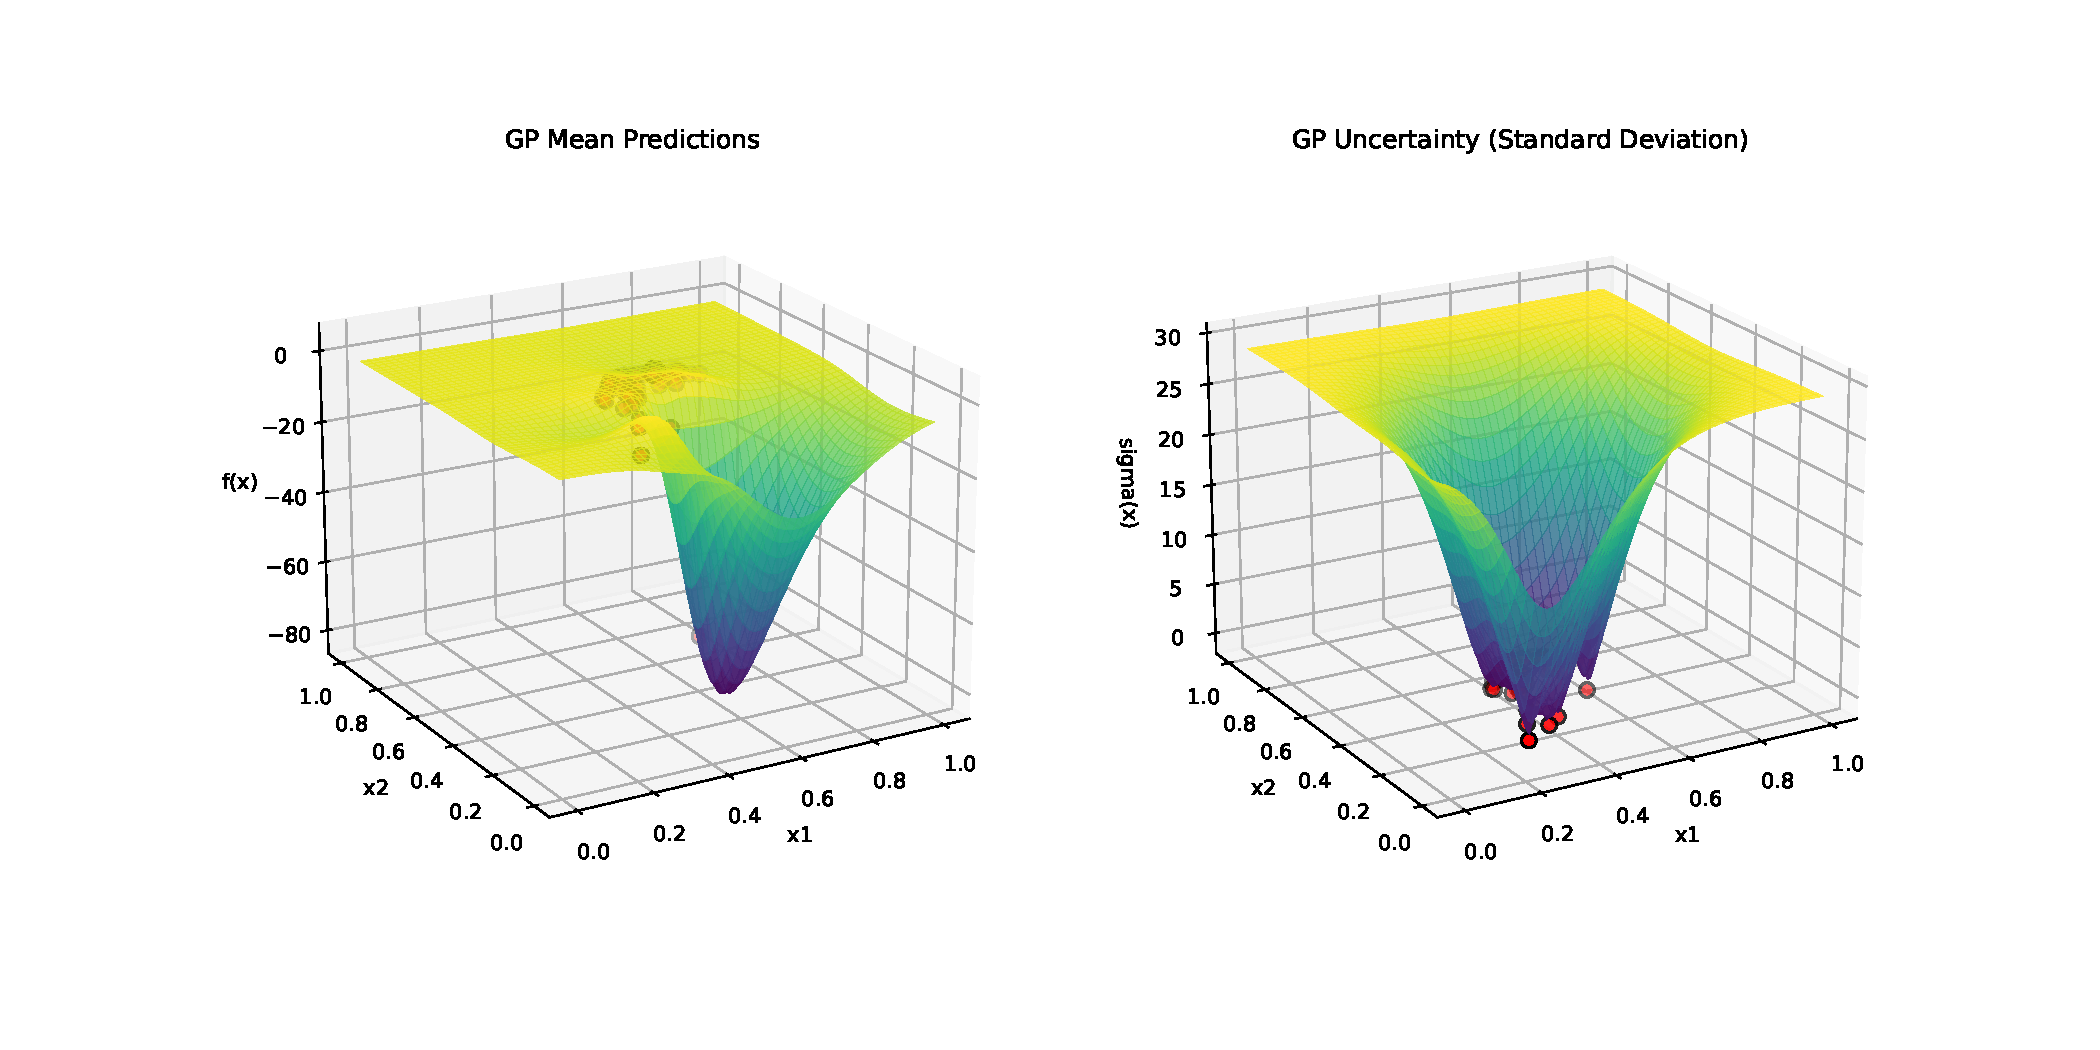
\includegraphics[width=\linewidth]{Bilder/appendix/3D_omp_0.6.pdf}
    \end{minipage} \\
    \begin{minipage}[c]{0.5\linewidth}
        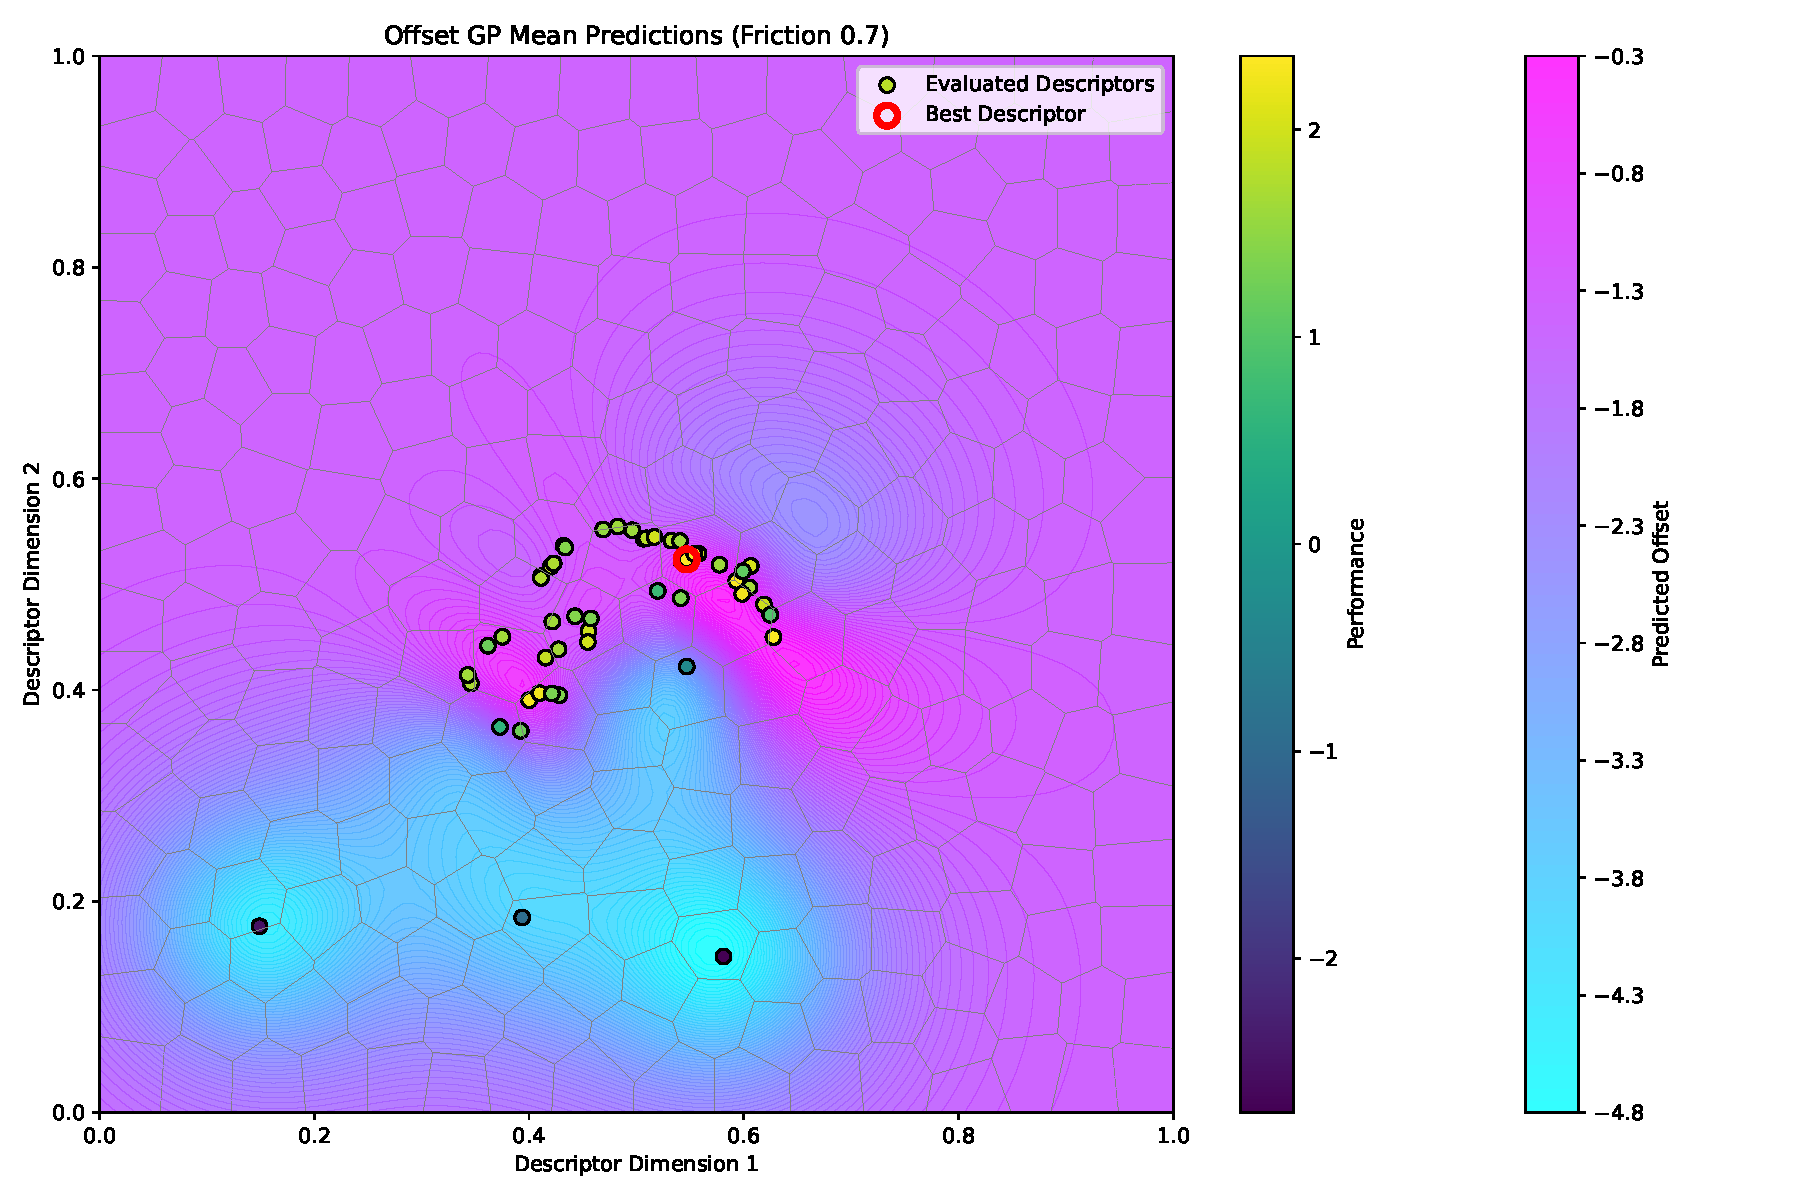
\includegraphics[width=\linewidth]{Bilder/appendix/omp_0.7.pdf}
    \end{minipage} &
    \begin{minipage}[c]{0.5\linewidth}
        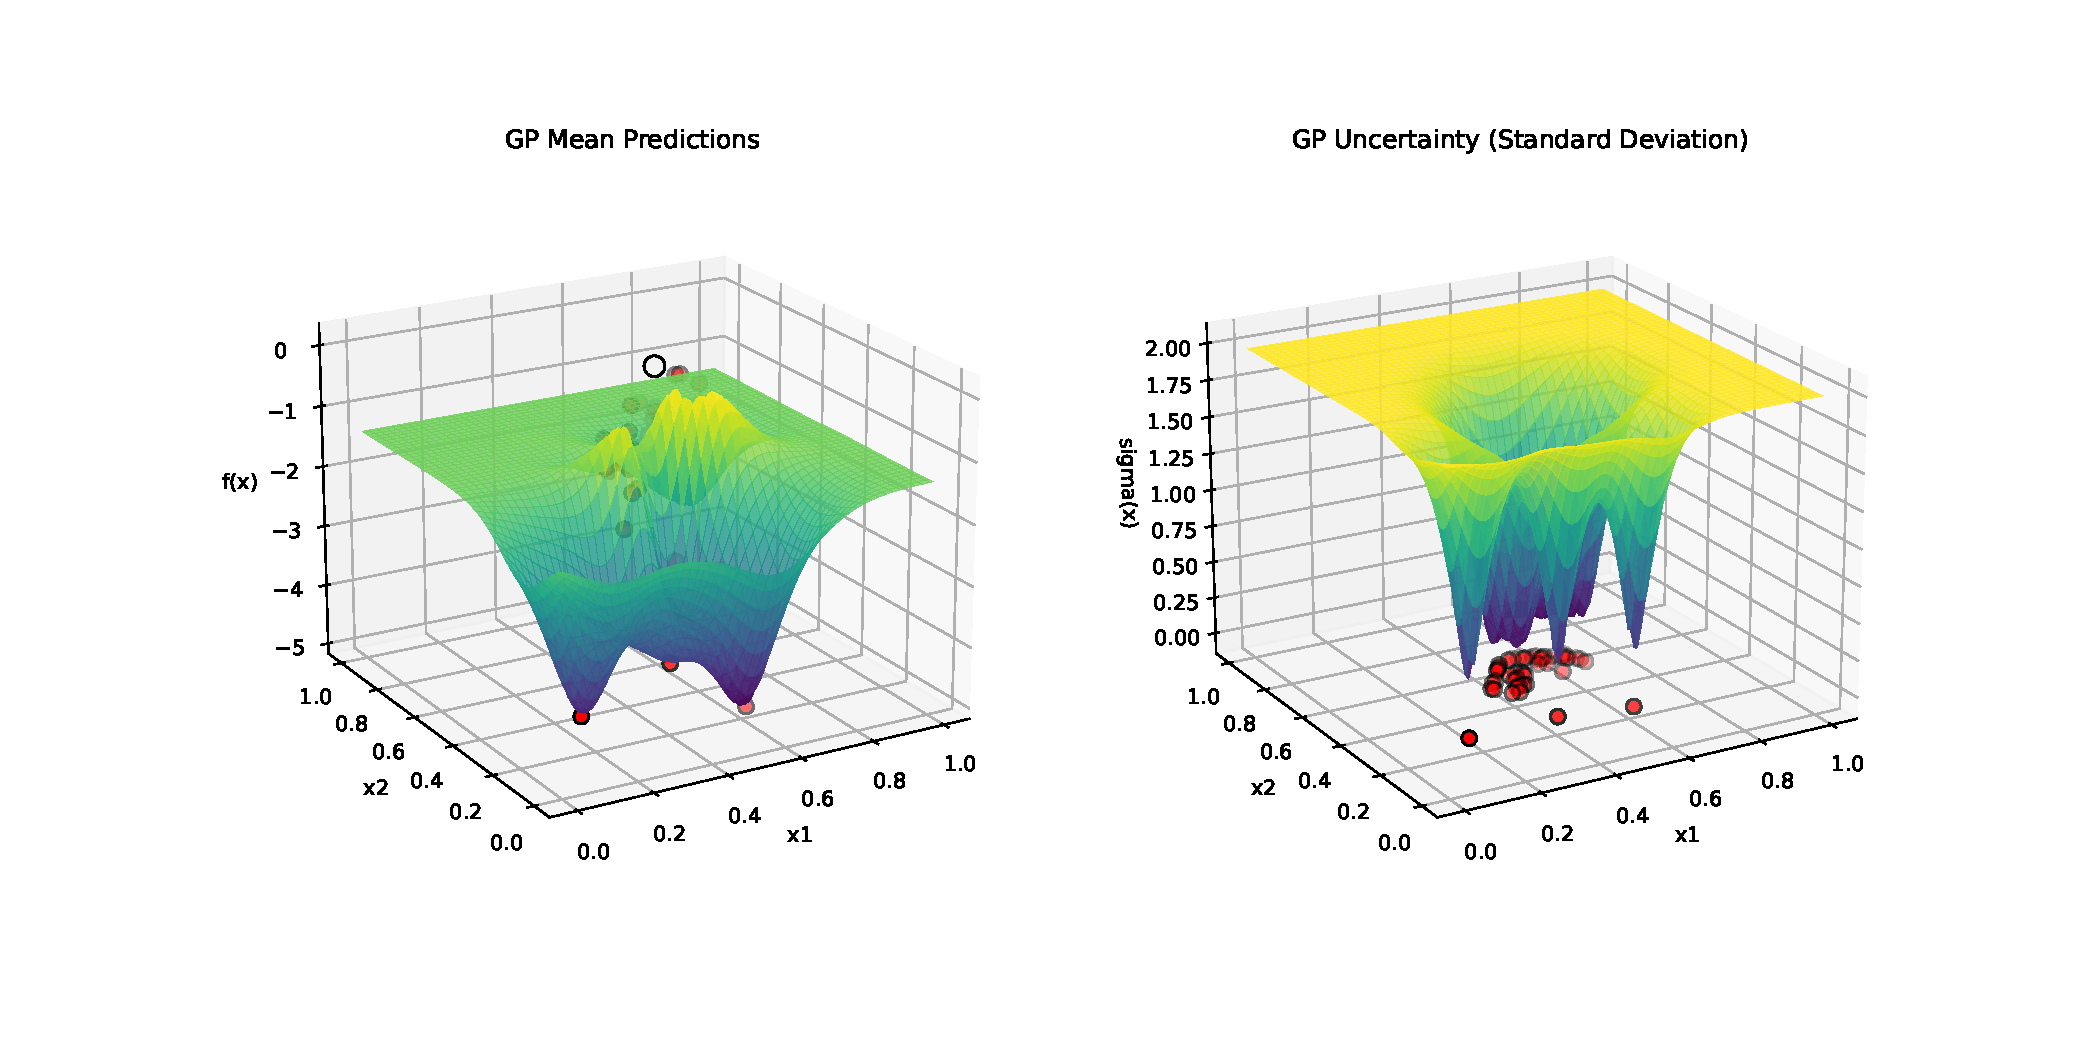
\includegraphics[width=\linewidth]{Bilder/appendix/3D_omp_0.7.pdf}
    \end{minipage} \\
    \begin{minipage}[c]{0.5\linewidth}
        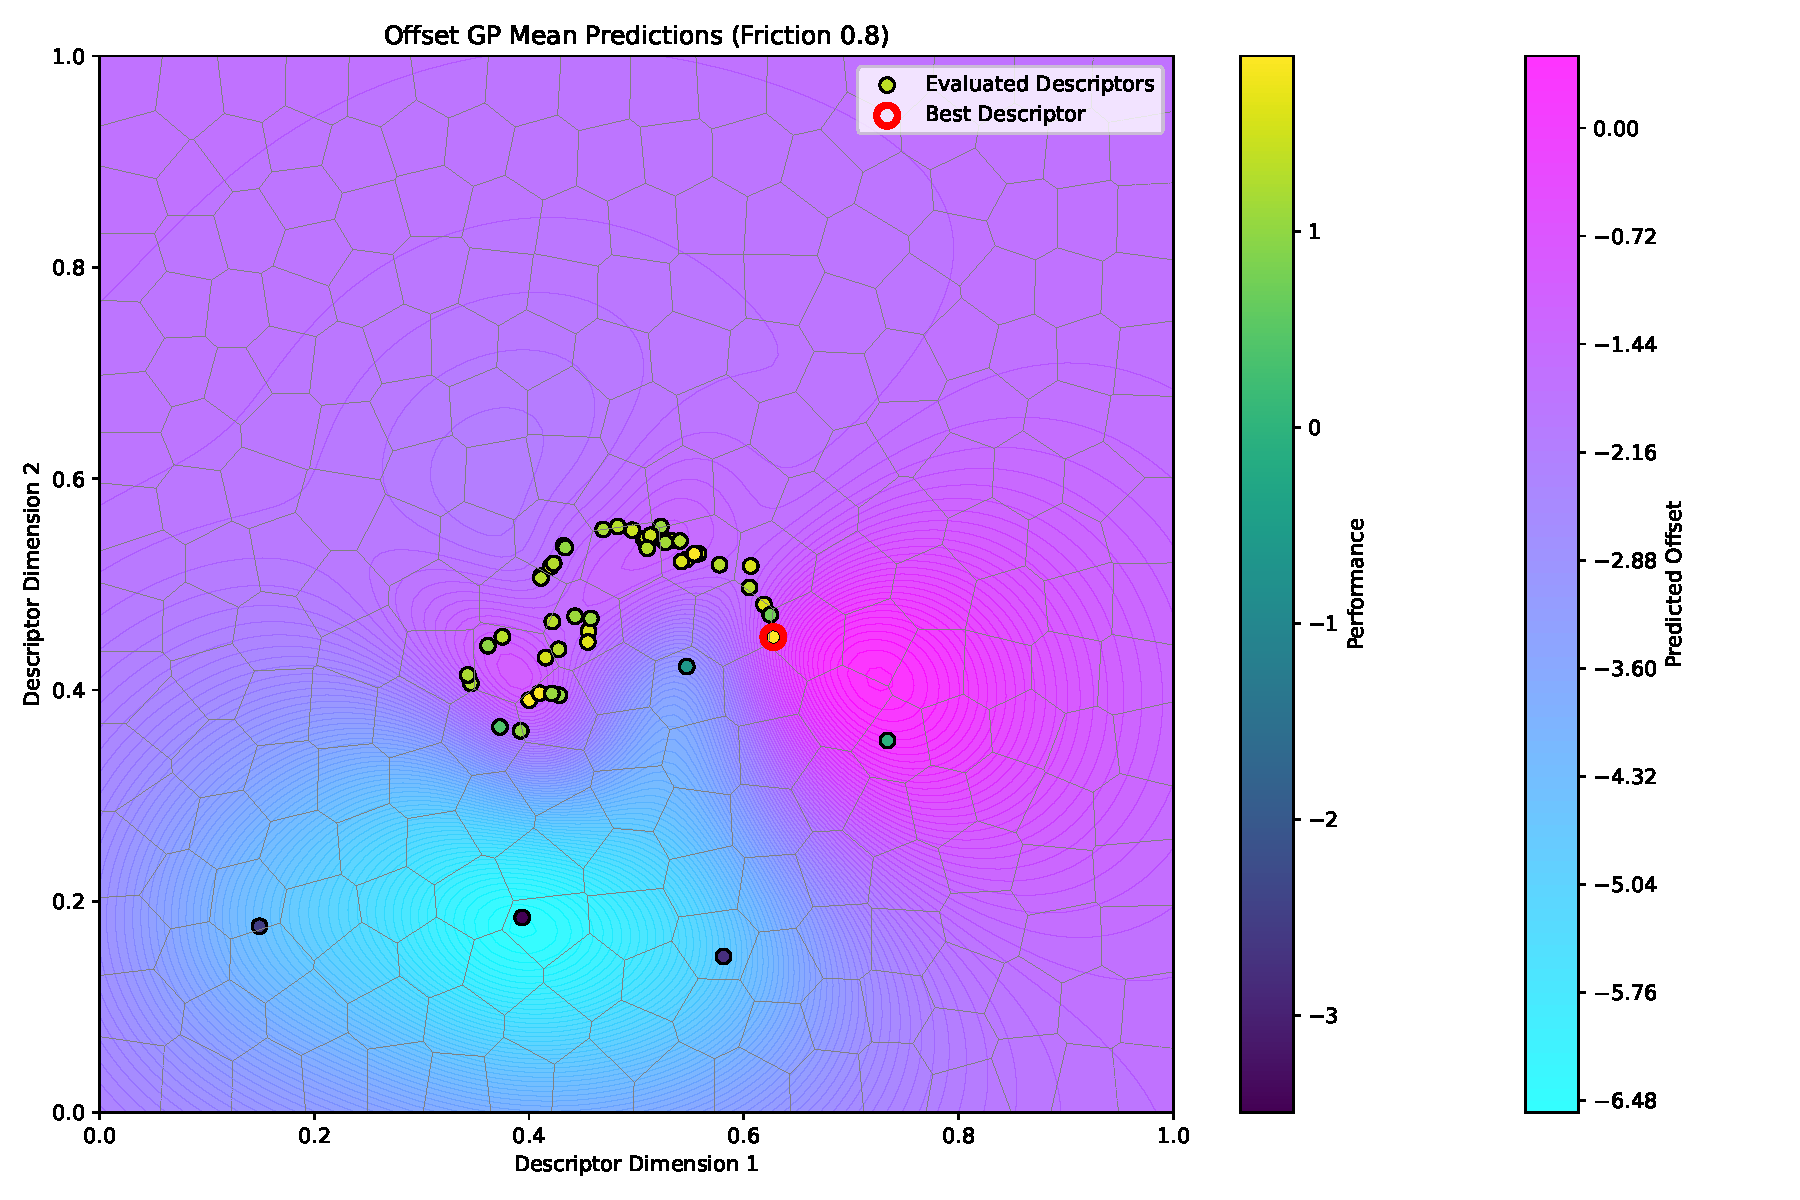
\includegraphics[width=\linewidth]{Bilder/appendix/omp_0.8.pdf}
    \end{minipage} &
    \begin{minipage}[c]{0.5\linewidth}
        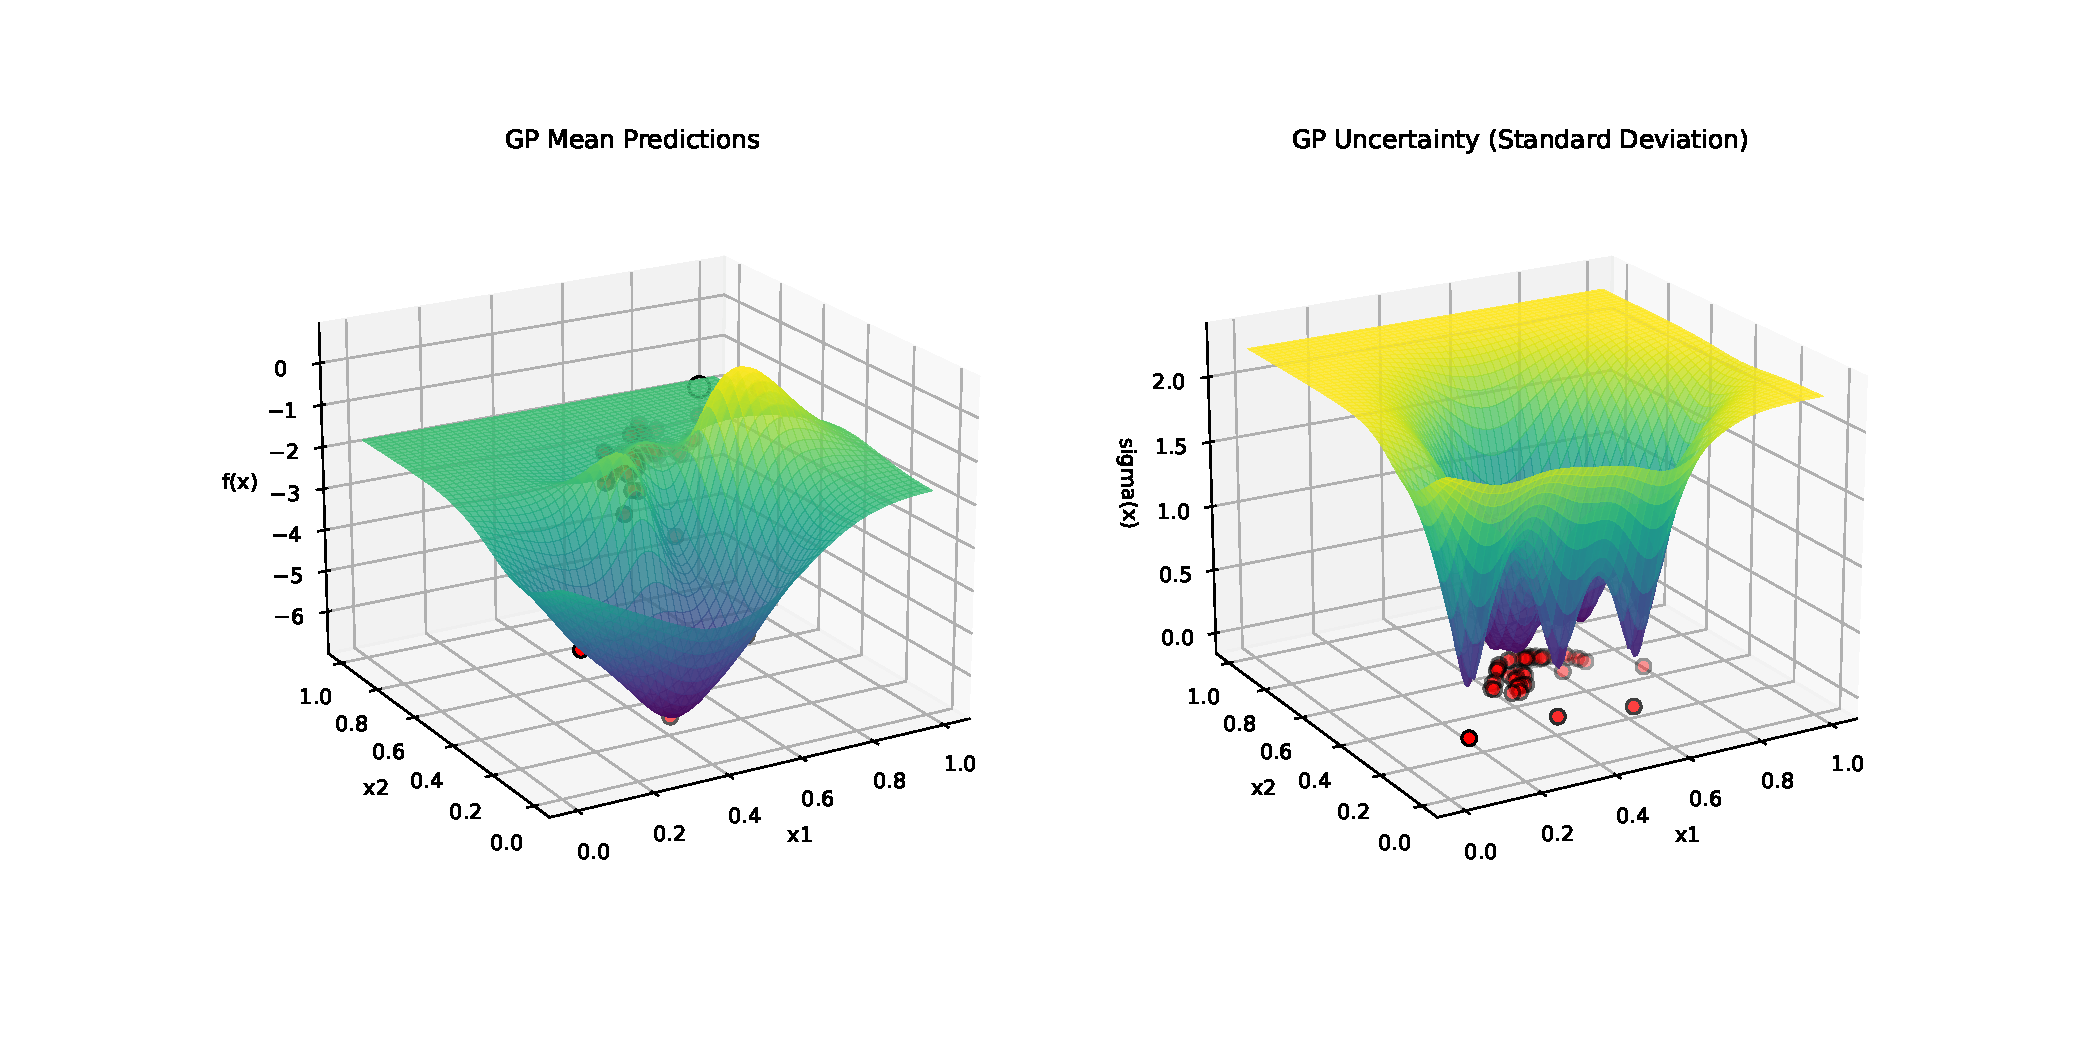
\includegraphics[width=\linewidth]{Bilder/appendix/3D_omp_0.8.pdf}
    \end{minipage} \\
    \begin{minipage}[c]{0.5\linewidth}
        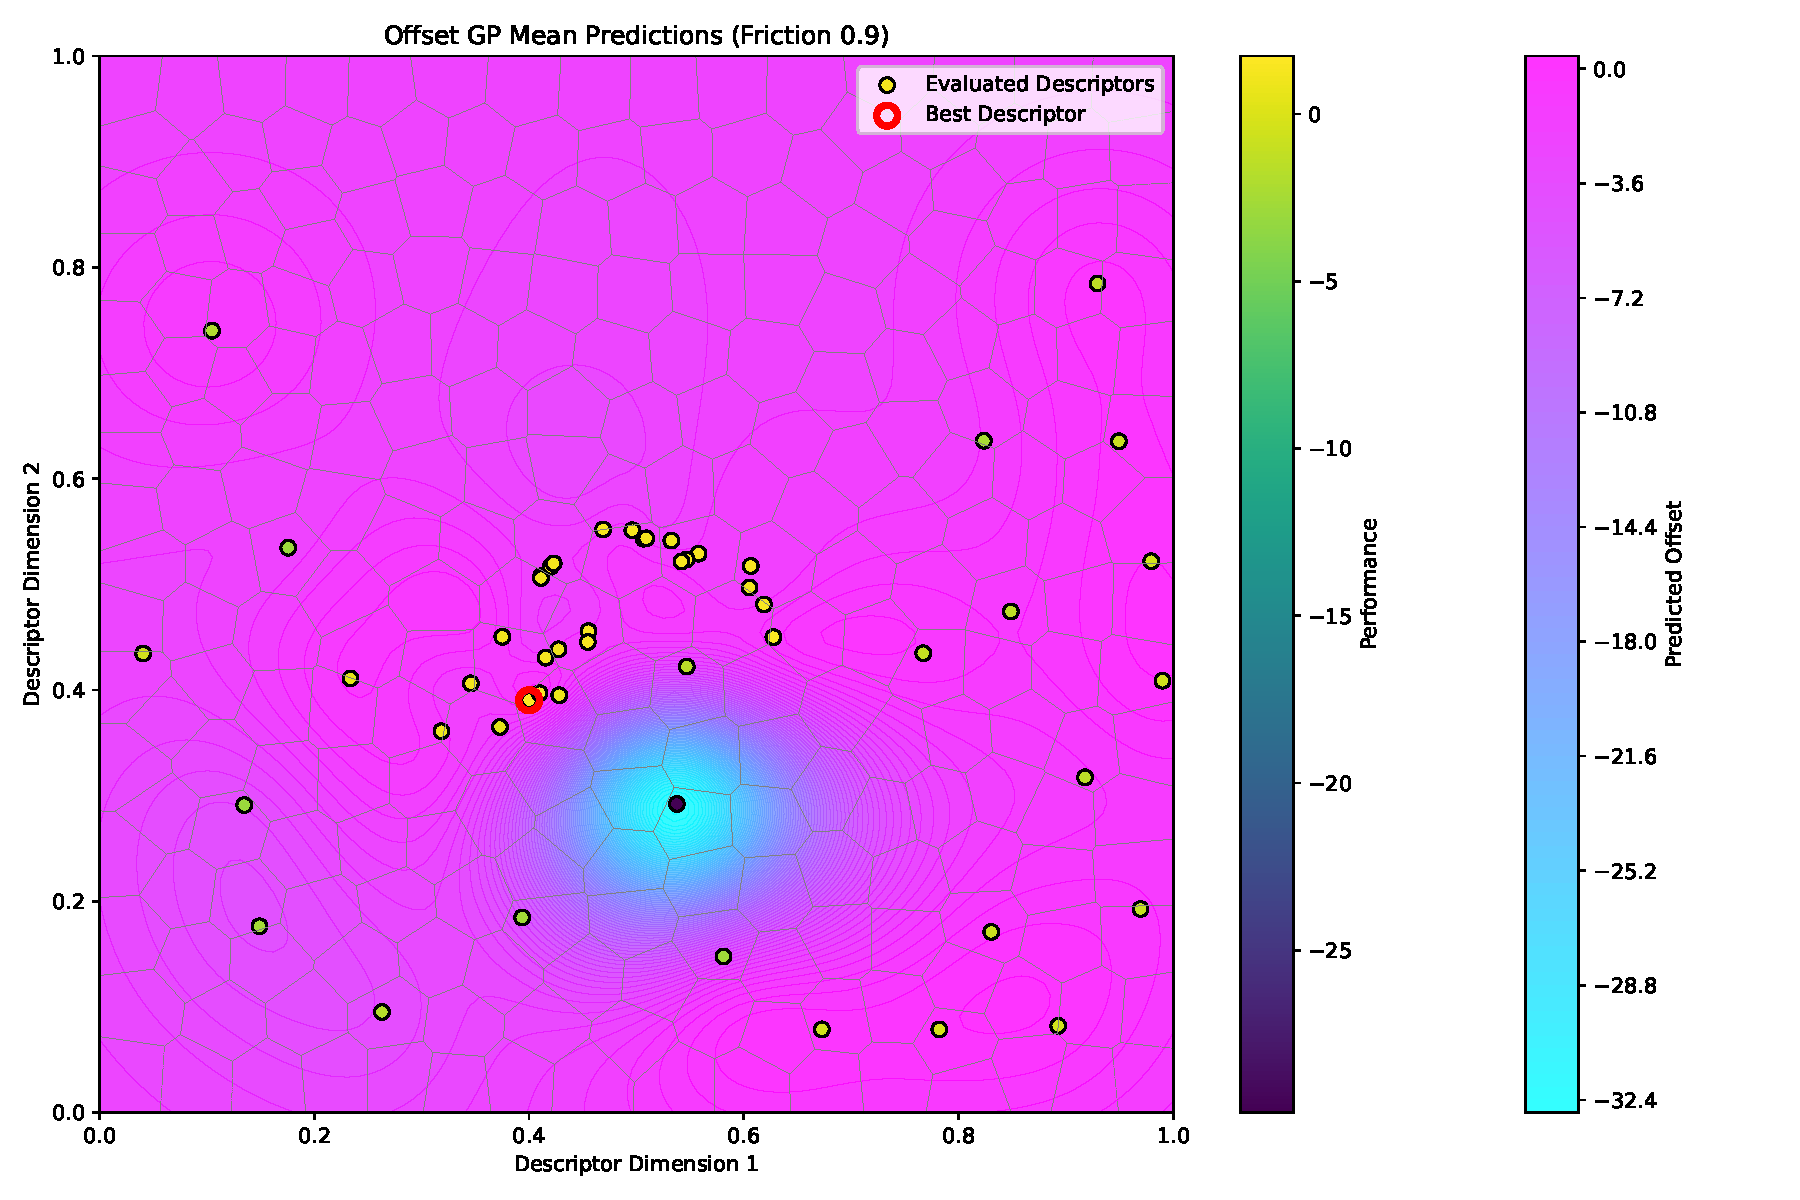
\includegraphics[width=\linewidth]{Bilder/appendix/omp_0.9.pdf}
    \end{minipage} &
    \begin{minipage}[c]{0.5\linewidth}
        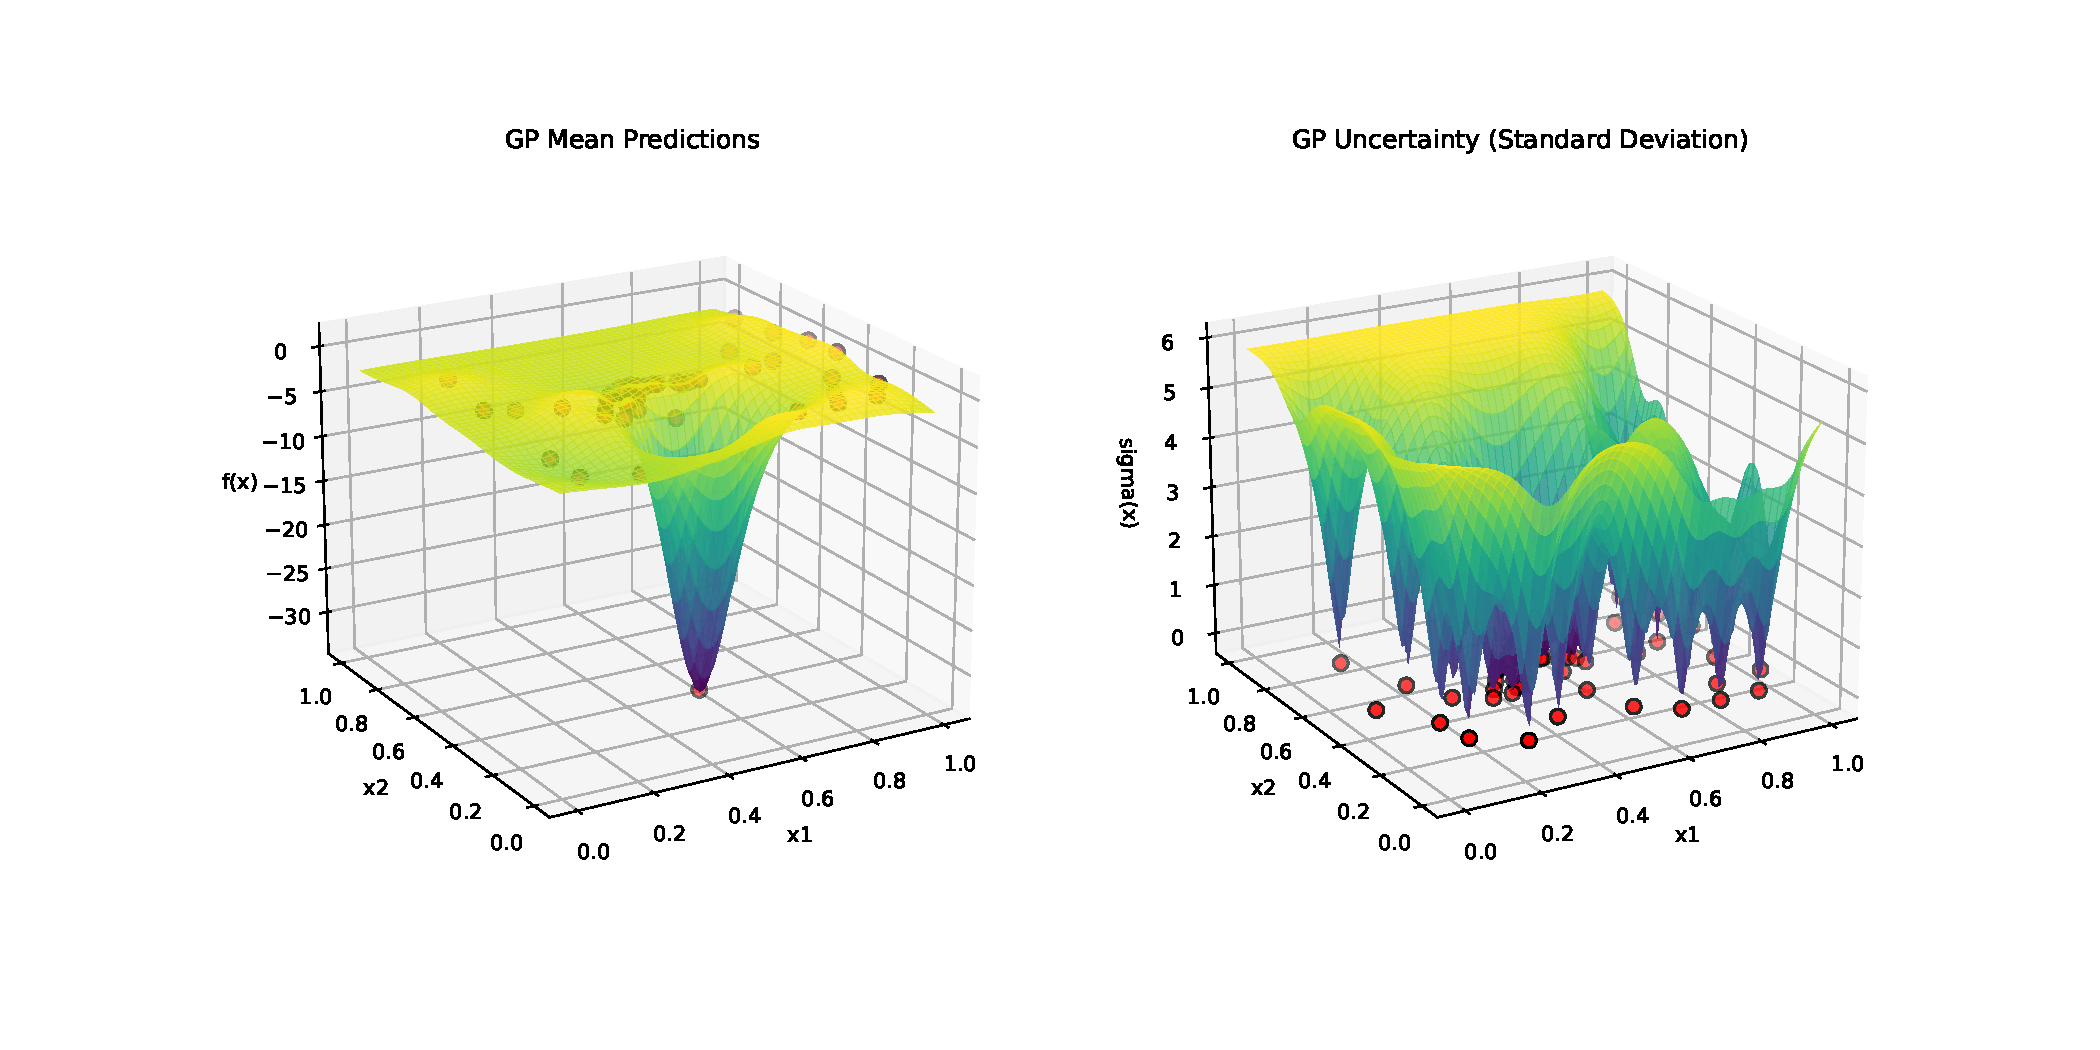
\includegraphics[width=\linewidth]{Bilder/appendix/3D_omp_0.9.pdf}
    \end{minipage} \\
    \caption{Gaussian Processes offset predictions for different frictions values. Left: Tested solutions with the dot color representing their performance in reality and the contour map is the GP predicted mean. Right: 3D representation of the predicted mean and uncertainty. }
\end{longtable}



\end{document}